\documentclass[11pt,a4paper]{article}

% ============================================================
%  Printing_Parameters_Textbook_v3.tex
%  "From Rheology to Scaffold: Engineering Principles and
%   Operating Guide for DIW Bioprinting of CMC / Sunflower-Oil
%   Nanoemulsion Bioinks"
%
%  Improvements over v2 (v3 = didactic theory overhaul):
%   - Three-tier teaching model (applied / mixed / graduate-research)
%   - "How to read this book - three paths" front matter
%   - Theory chapters rebuilt on a 10-beat didactic arc
%   - New tiers: IN PRACTICE, GOING DEEPER; level-tagged EXERCISES + solutions toggle
%   - New theory taught: Cox-Merz, yield-stress methods, relaxation time,
%     N1/Tanner die swell, Arrhenius/WLF, Krieger-Dougherty, Metzner-Reed Re, Mooney slip
%   - New section: Temperature & Process-Robustness
%  Author: T. M. C. Rodrigues, PEMM/COPPE/UFRJ | Date: 2026-06-07 | Version 3.0
% ============================================================

% ----- Packages -----
\usepackage[utf8]{inputenc}
\usepackage[T1]{fontenc}
\usepackage{lmodern}
\usepackage[margin=2.3cm]{geometry}
\usepackage{amsmath,amssymb,amsfonts}
\usepackage{siunitx}
\usepackage{booktabs}
\usepackage{multirow}
\usepackage{array}
\usepackage{graphicx}
\usepackage{listings}
\usepackage{xcolor}
\definecolor{indigo}{RGB}{75,0,130}
\usepackage{hyperref}
\usepackage{caption}
\usepackage{subcaption}
\usepackage{enumitem}
\usepackage{verbatim}
\usepackage{environ}
\usepackage{tcolorbox}
\usepackage{fancyhdr}
\usepackage{titlesec}
\usepackage[round]{natbib}
\usepackage{lastpage}
\usepackage{tikz}
\usepackage{longtable}
\usepackage{tabularx}
\usetikzlibrary{arrows.meta,positioning,calc,shapes.geometric,fit,decorations.pathreplacing}

% ----- Hyperref -----
\hypersetup{
  colorlinks=true,
  linkcolor=blue!50!black,
  urlcolor=blue!60!black,
  citecolor=teal!50!black
}

% ----- Colored boxes -----
\tcbuselibrary{skins,breakable}

\newtcolorbox{intuitionbox}[1][]{
  colback=yellow!8!white, colframe=yellow!55!black,
  fonttitle=\bfseries, coltitle=white, colbacktitle=yellow!55!black,
  title={PHYSICAL INTUITION}, arc=2mm, boxrule=0.5pt,
  left=8pt, right=8pt, top=4pt, bottom=4pt, breakable, #1
}

\newtcolorbox{examplebox}[1][]{
  colback=blue!4!white, colframe=blue!55!black,
  fonttitle=\bfseries, coltitle=white, colbacktitle=blue!55!black,
  title={WORKED EXAMPLE -- the three inks}, arc=2mm, boxrule=0.5pt,
  left=8pt, right=8pt, top=4pt, bottom=4pt, breakable, #1
}

\newtcolorbox{derivationbox}[1][]{
  colback=gray!6!white, colframe=gray!55!black,
  fonttitle=\bfseries, coltitle=white, colbacktitle=gray!55!black,
  title={DERIVATION}, arc=2mm, boxrule=0.5pt,
  left=8pt, right=8pt, top=4pt, bottom=4pt, breakable, #1
}

\newtcolorbox{stepbox}[2][]{
  colback=teal!5!white, colframe=teal!55!black,
  fonttitle=\bfseries, coltitle=white, colbacktitle=teal!55!black,
  title={#2}, arc=2mm, boxrule=0.5pt,
  left=8pt, right=8pt, top=4pt, bottom=4pt, breakable, #1
}

\newtcolorbox{stopcheck}[1][]{
  colback=orange!8!white, colframe=orange!75!black,
  fonttitle=\bfseries, coltitle=white, colbacktitle=orange!75!black,
  title={STOP \& CHECK}, arc=2mm, boxrule=0.5pt,
  left=8pt, right=8pt, top=4pt, bottom=4pt, breakable, #1
}

\newtcolorbox{warningbox}[1][]{
  colback=red!6!white, colframe=red!70!black,
  fonttitle=\bfseries, coltitle=white, colbacktitle=red!70!black,
  title={SAFETY / DATA INTEGRITY}, arc=2mm, boxrule=0.5pt,
  left=8pt, right=8pt, top=4pt, bottom=4pt, breakable, #1
}

\newtcolorbox{tipbox}[1][]{
  colback=green!5!white, colframe=green!50!black,
  fonttitle=\bfseries, coltitle=white, colbacktitle=green!50!black,
  title={TIP}, arc=2mm, boxrule=0.5pt,
  left=8pt, right=8pt, top=4pt, bottom=4pt, breakable, #1
}

\newtcolorbox{controlbox}[1][]{
  colback=purple!4!white, colframe=purple!55!black,
  fonttitle=\bfseries, coltitle=white, colbacktitle=purple!55!black,
  title={CONTROL PARADIGM}, arc=2mm, boxrule=0.5pt,
  left=8pt, right=8pt, top=4pt, bottom=4pt, breakable, #1
}

\newtcolorbox{runningbox}[2][]{
  colback=violet!4!white, colframe=violet!55!black,
  fonttitle=\bfseries, coltitle=white, colbacktitle=violet!55!black,
  title={#2}, arc=2mm, boxrule=0.5pt,
  left=8pt, right=8pt, top=4pt, bottom=4pt, breakable, #1
}

% --- NEW box types (v2) ---
\newtcolorbox{takeawaybox}[1][]{
  colback=cyan!5!white, colframe=cyan!60!black,
  fonttitle=\bfseries, coltitle=white, colbacktitle=cyan!60!black,
  title={KEY TAKEAWAYS}, arc=2mm, boxrule=0.5pt,
  left=8pt, right=8pt, top=4pt, bottom=4pt, breakable, #1
}

\newtcolorbox{designrulebox}[1][]{
  colback=olive!5!white, colframe=olive!65!black,
  fonttitle=\bfseries, coltitle=white, colbacktitle=olive!65!black,
  title={ENGINEERING DESIGN RULES}, arc=2mm, boxrule=0.5pt,
  left=8pt, right=8pt, top=4pt, bottom=4pt, breakable, #1
}

\newtcolorbox{dimensionlessbox}[1][]{
  colback=brown!4!white, colframe=brown!55!black,
  fonttitle=\bfseries, coltitle=white, colbacktitle=brown!55!black,
  title={DIMENSIONLESS ANALYSIS}, arc=2mm, boxrule=0.5pt,
  left=8pt, right=8pt, top=4pt, bottom=4pt, breakable, #1
}

\newtcolorbox{failurebox}[2][]{
  colback=red!3!white, colframe=red!55!black,
  fonttitle=\bfseries, coltitle=white, colbacktitle=red!55!black,
  title={FAILURE MODE: #2}, arc=2mm, boxrule=0.5pt,
  left=8pt, right=8pt, top=4pt, bottom=4pt, breakable, #1
}

\newtcolorbox{interactionbox}[1][]{
  colback=magenta!3!white, colframe=magenta!50!black,
  fonttitle=\bfseries, coltitle=white, colbacktitle=magenta!50!black,
  title={PARAMETER INTERACTIONS}, arc=2mm, boxrule=0.5pt,
  left=8pt, right=8pt, top=4pt, bottom=4pt, breakable, #1
}

% --- NEW tiers (v3): in-practice, going-deeper, exercises, solutions toggle ---
\newtcolorbox{inpracticebox}[1][]{
  colback=teal!4!white, colframe=teal!60!black,
  fonttitle=\bfseries, coltitle=white, colbacktitle=teal!60!black,
  title={IN PRACTICE}, arc=2mm, boxrule=0.5pt,
  left=8pt, right=8pt, top=4pt, bottom=4pt, breakable, #1
}
\newtcolorbox{goingdeeperbox}[1][]{
  colback=indigo!5!white, colframe=indigo!60!black,
  fonttitle=\bfseries, coltitle=white, colbacktitle=indigo!60!black,
  title={GOING DEEPER}, arc=2mm, boxrule=0.5pt,
  left=8pt, right=8pt, top=4pt, bottom=4pt, breakable, #1
}

% Difficulty markers for exercises
\newcommand{\diffA}{\textcolor{green!55!black}{$\circ$}}
\newcommand{\diffB}{\textcolor{orange!80!black}{$\circ\circ$}}
\newcommand{\diffC}{\textcolor{red!70!black}{$\circ\circ\circ$}}

% Solutions toggle: student build by default; instructor build via \def\SOLUTIONS{1}
\providecommand{\SOLUTIONS}{0}
\newif\ifsolutions
\ifnum\SOLUTIONS=1 \solutionstrue \else \solutionsfalse \fi

% Exercise environment (counter per section)
\newcounter{exidx}[section]
\renewcommand{\theexidx}{\thesection.\arabic{exidx}}
\newenvironment{exercise}[1]%
  {\par\smallskip\refstepcounter{exidx}%
   \noindent\textbf{Exercise~\theexidx}~#1\quad}
  {\par\smallskip}

% Solution box (instructor build only) — robust implementation via environ package
\newtcolorbox{solutionbox}[1][]{
  colback=gray!3!white, colframe=green!45!black,
  fonttitle=\bfseries, coltitle=white, colbacktitle=green!45!black,
  title={SOLUTION}, arc=1mm, boxrule=0.4pt,
  left=8pt, right=8pt, top=3pt, bottom=3pt, breakable, #1
}
\NewEnviron{solution}{%
  \ifsolutions\begin{solutionbox}\BODY\end{solutionbox}\fi%
}

% ----- Headers -----
\pagestyle{fancy}
\fancyhf{}
\rhead{\small Textbook v3.0 -- DIW Printing of CMC/NE Bioinks}
\lhead{\small BioPoli -- PEMM/COPPE/UFRJ}
\rfoot{\small \thepage\,/\,\pageref{LastPage}}
\renewcommand{\headrulewidth}{0.4pt}

% ----- Math shorthands -----
\newcommand{\gd}{\dot{\gamma}}
\newcommand{\Pas}{\,\mathrm{Pa\,s}}
\newcommand{\mms}{\,\mathrm{mm/s}}
\newcommand{\Bi}{\mathrm{Bi}}
\newcommand{\Rey}{\mathrm{Re}}
\newcommand{\De}{\mathrm{De}}
\newcommand{\Ca}{\mathrm{Ca}}

% ----- Listings -----
\lstdefinestyle{shell}{
  basicstyle=\ttfamily\footnotesize,
  backgroundcolor=\color{gray!8},
  frame=single, rulecolor=\color{gray!40},
  columns=fullflexible, breaklines=true,
  showstringspaces=false, tabsize=2
}

% ----- Titles -----
\titlespacing*{\section}{0pt}{14pt}{6pt}
\titlespacing*{\subsection}{0pt}{10pt}{4pt}

\title{\textbf{From Rheology to Scaffold}\\[4pt]
\large \textsl{Engineering Principles and Operating Guide for Direct
Ink Writing of CMC / Sunflower-Oil Nanoemulsion Bioinks}\\[4pt]
\normalsize \textsl{Theory, dimensionless analysis, three worked-example inks,
failure morphology, nanoemulsion mechanics, biological considerations,
lab protocols, and troubleshooting}}
\author{T.~M.~C.~Rodrigues \and R.~Thir\'e \\[2pt]
\small BioPoli -- PEMM/COPPE/UFRJ \\[2pt]
\small Version 3.0 \quad \today}
\date{}

\begin{document}
\maketitle
\thispagestyle{fancy}

\begin{tcolorbox}[colback=blue!3!white,colframe=blue!50!black,
                  arc=2mm,boxrule=0.4pt,left=8pt,right=8pt]
\textbf{Who this document is for and how to use it.}\\
This is a self-contained engineering guide to printing CMC and
CMC\,+\,sunflower-oil nanoemulsion bioinks on the piston-driven DIW gel
printer. It is written for a new lab member or intern with an
undergraduate engineering background (basic calculus, basic fluid
mechanics) and no prior rheology experience. It is also a reference for
experienced practitioners seeking a rigorous foundation for material
selection, process parameter estimation, failure diagnosis, and regulatory
justification.

\medskip
The document is in four parts:
\begin{itemize}[leftmargin=1.4em,itemsep=2pt]
\item \textbf{Part I -- Theory} (Ch.~1--7): step-by-step engineering
framework connecting rheological measurements to printing parameters.
Includes failure morphology and dimensionless analysis.
\item \textbf{Part II -- Inks and Instruments} (Ch.~8--11): ink
characterisation, nanoemulsion mechanics, rheological testing protocols,
and extended material classes.
\item \textbf{Part III -- Protocols} (Ch.~12--17): MATLAB and Python
workflows, calibration-cube sequence, and troubleshooting decision tree.
\item \textbf{Part IV -- Extended Topics} (Ch.~18--19): biological and
regulatory considerations; statistical optimisation methods.
\end{itemize}

\medskip
\textbf{Navigation guide.} If you only need to print and trust the
upstream calibration, skip to Part~III. If a print fails and you do not
understand why, the answer is in Part~I, Chapter~7. If you are preparing
a manuscript or patent, Part~IV is mandatory reading.
\end{tcolorbox}

\tableofcontents
\bigskip\hrule\bigskip

\clearpage
\section*{How to Read This Book --- Three Paths}
\addcontentsline{toc}{section}{How to Read This Book --- Three Paths}

This book teaches at three depths from one text. Read the \emph{core spine}
(plain text, worked examples, takeaways, design rules) on any path; then add
the tiers your role needs.

\begin{center}\small
\begin{tabular}{p{3.2cm} p{4.0cm} p{5.6cm}}
\toprule
\textbf{Tier (badge)} & \textbf{What it gives you} & \textbf{Who should read it} \\
\midrule
Core spine & Intuition, the result, real numbers, takeaways & \textbf{Everyone} \\
\rule{0pt}{2.4ex}\textsc{In Practice} (teal) & Bench-level ``what you actually do'' & \textbf{Applied} + everyone \\
\textsc{Derivation} (grey) & Full step-by-step proof of the result & \textbf{Graduate-research}; skippable on first read \\
\textsc{Going Deeper} (indigo) & Advanced connections (Cox--Merz, $N_1$/Tanner, structural kinetics) & \textbf{Graduate-research} / curious \\
Exercises \diffA\,\diffB\,\diffC & Self-check, by difficulty & By level; solutions in instructor edition \\
\bottomrule
\end{tabular}
\end{center}

\begin{center}\small
\begin{tabular}{ll}
\toprule
\textbf{Profile} & \textbf{Suggested path} \\
\midrule
Applied / practitioner & Core spine + \textsc{In Practice} + \diffA exercises \\
Mixed (grad/adv.\ undergrad) & Core spine + \textsc{In Practice} + \textsc{Derivation} + \diffA\,\diffB \\
Graduate-research & All tiers + \textsc{Going Deeper} + \diffA\,\diffB\,\diffC \\
\bottomrule
\end{tabular}
\end{center}

\noindent\textbf{Instructors:} compile the solutions edition with
\texttt{pdflatex "\textbackslash def\textbackslash SOLUTIONS\{1\}\textbackslash input\{Printing\_Parameters\_Textbook\_v3.tex\}"}.

% =================================================================
%  SYSTEMS-LEVEL FRAMEWORK
% =================================================================
\section*{Conceptual Framework: DIW as a Coupled System}
\addcontentsline{toc}{section}{Conceptual Framework: DIW as a Coupled System}
\label{sec:framework}

Direct Ink Writing is not a single-physics problem. It is a
\textbf{coupled system} in which formulation chemistry, network
rheology, extrusion hydraulics, deposition geometry, and scaffold
mechanics interact simultaneously. Every printing parameter is both a
cause and a consequence in this web. The central thesis of this textbook
is: \emph{understand the coupling, and every slicer entry follows by
algebra.}

Figure~\ref{fig:systems} shows the complete coupling map.

\begin{figure}[h]
\centering
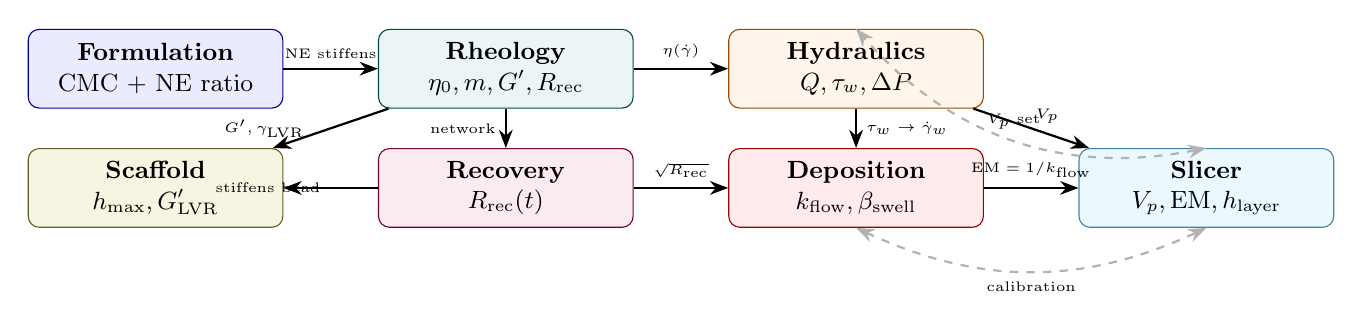
\begin{tikzpicture}[
  node distance=5mm and 12mm,
  every node/.style={font=\small},
  box/.style={draw, rounded corners, text width=3.0cm, align=center,
              minimum height=1.0cm, fill=#1!8, draw=#1!60!black},
  arr/.style={-Stealth, thick},
  darr/.style={Stealth-Stealth, thick, dashed, draw=gray!60}
]
  % Nodes
  \node[box=blue]   (form) {\textbf{Formulation}\\CMC + NE ratio};
  \node[box=teal,   right=of form] (rheo) {\textbf{Rheology}\\$\eta_0,m,G',R_\mathrm{rec}$};
  \node[box=orange, right=of rheo] (hydro) {\textbf{Hydraulics}\\$Q,\tau_w,\Delta P$};
  \node[box=red,    below=of hydro] (dep)  {\textbf{Deposition}\\$k_\mathrm{flow},\beta_\mathrm{swell}$};
  \node[box=purple, below=of rheo]  (recov) {\textbf{Recovery}\\$R_\mathrm{rec}(t)$};
  \node[box=olive,  below=of form]  (scaf) {\textbf{Scaffold}\\$h_\mathrm{max},G'_\mathrm{LVR}$};
  \node[box=cyan,   right=of dep]   (slicer) {\textbf{Slicer}\\$V_p,\mathrm{EM},h_\mathrm{layer}$};
  % Arrows
  \draw[arr] (form) -- (rheo) node[midway,above]{\tiny NE stiffens};
  \draw[arr] (rheo) -- (hydro) node[midway,above]{\tiny $\eta(\gd)$};
  \draw[arr] (hydro) -- (dep) node[midway,right]{\tiny $\tau_w\to\gd_w$};
  \draw[arr] (rheo) -- (recov) node[midway,left]{\tiny network};
  \draw[arr] (recov) -- (dep) node[midway,above]{\tiny $\sqrt{R_\mathrm{rec}}$};
  \draw[arr] (recov) -- (scaf) node[midway,left]{\tiny stiffens bead};
  \draw[arr] (rheo) -- (scaf) node[midway,left=2mm]{\tiny $G',\gamma_\mathrm{LVR}$};
  \draw[arr] (dep) -- (slicer) node[midway,above]{\tiny $\mathrm{EM}=1/k_\mathrm{flow}$};
  \draw[arr] (hydro) -- (slicer) node[midway,above right=-1mm]{\tiny $V_p$};
  % Feedback
  \draw[darr] (slicer.north) to[bend left=30] node[above,font=\tiny]{$V_p$ set} (hydro.north);
  \draw[darr] (dep.south) to[bend right=25] node[below,font=\tiny]{calibration} (slicer.south);
\end{tikzpicture}
\caption{Systems-level coupling map for piston-driven DIW.
Solid arrows: physical causation. Dashed: feedback via calibration or operator control.
The operator directly commands only $V_p$ (piston velocity); every other quantity is
a consequence of the ink's rheology and the system geometry.}
\label{fig:systems}
\end{figure}

\begin{interactionbox}
\textbf{How parameters couple -- the four most important interactions.}
\begin{enumerate}[leftmargin=1.6em,itemsep=3pt]
\item \textbf{Increasing $V_p$ raises $Q$, which raises $\gd_w$, which
lowers $\eta$ (shear thinning), which raises $\tau_w$ sub-linearly.}
Pressure does not scale linearly with $V_p$ for shear-thinning inks:
doubling $V_p$ typically increases $\Delta P$ by a factor of
$2^n$ ($n<1$).
\item \textbf{Increasing $V_p$ also raises $v_\mathrm{print}$, which
shortens dwell time per layer, which changes the SAOS criterion
controlling $h_\mathrm{scaffold}^\mathrm{max}$.} Faster printing can
mean the $G'(\omega=1)$ criterion applies rather than the
$G'(\omega=0.01)$ one -- apparently improving height capacity.
\item \textbf{Adding NE raises $\eta_0$ and $G'_\mathrm{LVR}$ but
slightly lowers $R_\mathrm{rec}$.} The first two effects improve
scaffold height and resist gravity; the last increases the required
Extrusion Multiplier. Both directions must be tracked simultaneously.
\item \textbf{Narrower needle reduces $R_n$, massively raising $\Delta P$
($\propto R_n^{-4}$) and $\gd_w$ ($\propto R_n^{-3}$) at the same
$V_p$.} Switching from 21G to 22G at fixed $V_p$ raises wall shear
stress and may breach cell-safety thresholds even though the ink
parameters are unchanged.
\end{enumerate}
\end{interactionbox}

\begin{runningbox}{RUNNING EXAMPLE -- The Friday print}
\textbf{Monday, 9:00.} You are Ana, a new intern at BioPoli. Your
supervisor hands you a sealed jar of \emph{C15 Gira 5.5} (CMC +
sunflower-oil nanoemulsion ink, the \textbf{headline ink} of this
project), a 21G blunt needle, and the following brief:

\medskip
\textsl{``By Friday at 16:00 I need a printed solid block, roughly
$1\times 1\times 2$~cm$^3$, of this ink. The shape doesn't matter -- any
rectangular prism is fine. The Wednesday morning slot on the printer
is yours. Don't waste ink.''}

\medskip
Your job between now and Wednesday: extract, from the analysis scripts
and this book, every number you must type into the slicer. Wednesday:
calibrate at the bench. Thursday: print. Friday: document and deliver.

\medskip
By the end of this book you will have answered, in order:
\begin{enumerate}[leftmargin=1.6em,itemsep=1pt]
\item \textbf{Can this ink print at all?} (Ch.~\ref{sec:rheo_primer})
\item \textbf{What piston velocity $V_p$ should I command?} (Ch.~\ref{sec:hydraulic_loop})
\item \textbf{Is the resulting extrusion pressure safe?} (Ch.~\ref{sec:HP})
\item \textbf{What flow factor $k_\mathrm{flow}$ (and slicer Extrusion Multiplier) do I enter?} (Ch.~\ref{sec:flow_factor})
\item \textbf{Will a $20$\,mm-tall block survive its own weight?} (Ch.~\ref{sec:hmax})
\item \textbf{What does my Wednesday calibration morning look like?} (Ch.~\ref{sec:cubes})
\end{enumerate}
After each chapter above, you will find a box titled ``Running Example --
Solution to Q$N$'', solving one question with explicit numbers and
marking what is still unknown.
\end{runningbox}

% =================================================================
% PART I -- THEORY
% =================================================================
\part*{Part I -- Theory}
\addcontentsline{toc}{part}{Part I -- Theory}

% =================================================================
\section{Why DIW is Not FFF}
\label{sec:diw_vs_fff}

Direct Ink Writing (DIW) extrudes a viscous fluid through a needle and
relies on the fluid's own rheology to retain its shape after deposition.
Fused Filament Fabrication (FFF) melts a thermoplastic, extrudes it as a
controlled-diameter molten strand, and solidifies it on contact with the
cooler build plate. The two processes look similar (an extruder moves over
a build plate), but the physics is fundamentally different, and the slicer
firmware -- written for FFF -- does \emph{not} translate cleanly.

\begin{intuitionbox}
In FFF, the filament has a fixed diameter (1.75 or 2.85\,mm). The
extruder pushes a known length of filament, giving a known volume of melt.
``How much material was deposited?'' is answered by E-axis geometry alone.

In DIW, the ink is a free fluid in a syringe. ``How much material was
deposited?'' depends on: (i) how fast the piston moves; (ii) how the ink
responds to shear in the needle; (iii) how the deposited filament swells
or relaxes after leaving the needle; (iv) how the network recovers in the
time between deposition and the next layer.

The slicer knows none of that. It still thinks it is FFF. Our job is to
compute the right numbers \emph{outside} the slicer and feed them in as if
they were FFF parameters.
\end{intuitionbox}

\subsection{Three control modes, one printer family}

DIW printers differ in what the operator commands:

\begin{enumerate}[leftmargin=1.6em,itemsep=2pt]
\item \textbf{Pneumatic DIW.} Operator commands $\Delta P$ (the gas
pressure driving the syringe). Flow rate $Q$ is the consequence.
Dominant in academic literature; simpler hardware and lower cell stress
at constant pressure.
\item \textbf{Screw / progressive-cavity DIW.} Operator commands auger
rotation, which translates to a quasi-constant $Q$. Robust against air
bubbles; more expensive; common in commercial bioprinting.
\item \textbf{Piston / volumetric DIW.} Operator commands piston linear
velocity $V_p$ (via a stepper-motor lead screw). Volumetric flow $Q$ is
fixed by syringe geometry. $\Delta P$ is whatever the rheology demands.
\textbf{This is the lab's printer.}
\end{enumerate}

\begin{controlbox}
The lab DIW printer is \textbf{piston-driven / volumetric}. The single
flow input is the piston velocity $V_p$ (\si{\mm/\s}), entered into
the slicer firmware as the E-axis feedrate. Everything downstream --
$Q$, $\bar v_n$, $\tau_w$, $\Delta P$, $v_\mathrm{print}$ -- follows
from $V_p$ and the ink rheology. They are \textbf{outputs and
diagnostics}, not knobs.

\medskip
\textbf{Implication for literature reading.} A paper that says ``we
extruded at 100\,kPa'' must be translated to a $V_p$ on our printer
before the number is useful. The translation goes through the rheological
model (Ch.~\ref{sec:HP}).
\end{controlbox}

\begin{takeawaybox}
\begin{itemize}[leftmargin=1.4em,itemsep=2pt]
\item DIW is a rheology-dependent process; FFF slicers must be ``tricked''
  with pre-computed parameters.
\item On the lab printer, $V_p$ is the only flow control input.
  $\Delta P$ is a diagnostic, never a knob.
\item Comparing across literature requires knowing the control mode
  (pneumatic, screw, or piston).
\end{itemize}
\end{takeawaybox}

\begin{designrulebox}
\textbf{DR 1.1.} Before reading any DIW paper, identify the control
mode. Pneumatic data give pressure--flowrate relationships; piston data
give velocity--flowrate relationships. They are not interchangeable
without going through the constitutive model.

\textbf{DR 1.2.} Never enter $\Delta P$ directly into the slicer -- it
does not exist as a slicer input on this printer. If a calibration
strategy asks for a pressure setting, it was written for pneumatic DIW.
\end{designrulebox}

% =================================================================
\section{Rheology in Depth}
\label{sec:rheo_primer}

Rheology is the science of how matter deforms and flows. For DIW we need
seven concepts: stress, strain rate, viscosity, shear thinning, yield
stress, viscoelasticity, and structural recovery.

\subsection{Stress, strain, and strain rate}

\emph{Motivation.} Every pressure, velocity, and shape prediction in this
book is built on three quantities; confuse stress with strain rate, or
report a viscosity without the shear rate it was measured at, and every
downstream number is meaningless.

Place a fluid between two parallel plates separated by a gap $h$. Hold
the bottom plate fixed; slide the top plate at velocity $V$ under a
tangential force $F$ over area $A$. The fluid is subjected to:

\begin{itemize}[leftmargin=1.6em,itemsep=2pt]
\item a \textbf{shear stress} $\tau = F/A$, in pascals (\si{\Pa}),
\item a \textbf{shear strain rate} $\gd = V/h$, in inverse seconds
(\si{\per\s}).
\end{itemize}

For a Newtonian fluid the two are linearly related:
\begin{equation}
\tau \;=\; \eta\,\gd
\label{eq:newton}
\end{equation}
where $\eta$ (\si{\Pa\s}) is the dynamic viscosity. Water has
$\eta\approx \SI{e-3}{\Pa\s}$; honey, $\eta\approx \SI{10}{\Pa\s}$;
our CMC inks span $\eta\sim\SI{100}{\Pa\s}$ at high shear to
$\eta\sim\SI{e3}{\Pa\s}$ at rest -- four orders of magnitude.

\subsection{Yield stress and the two-viscosity problem}

\emph{Motivation.} Get this wrong and the ink either won't hold its shape
after deposition (no yield stress, so it slumps) or won't start flowing at
a safe pressure (too high a yield stress for the syringe). The yield stress
is the single number that decides which of those two failures you get.

Many structured fluids behave like solids at low stress and like
viscous fluids above a critical threshold called the \textbf{yield
stress} $\tau_y$. The simplest model is the Bingham fluid:
\begin{equation}
\tau \;=\; \tau_y \;+\; \eta_p\,\gd \qquad (\tau > \tau_y);
\qquad \gd = 0 \quad (\tau \leq \tau_y).
\label{eq:bingham}
\end{equation}

For DIW, a non-zero $\tau_y$ is advantageous: once extruded, the
material stops flowing at rest and holds its shape. The Herschel-Bulkley
model generalises this to power-law viscosity above yield:
\begin{equation}
\tau \;=\; \tau_y \;+\; K\,\gd^n \qquad (\tau > \tau_y).
\label{eq:HB}
\end{equation}

In practice, the inks in this project behave as \emph{apparent} yield
stress fluids: the zero-shear plateau of the Cross model ($\eta_0$) is
so high that the material appears solid on lab timescales. We do not
formally fit $\tau_y$ but we extract an equivalent from SAOS data
(Ch.~\ref{sec:hmax}).

\begin{derivationbox}
\textbf{Why $\tau_y \approx G'_\mathrm{LVR}\,\gamma_\mathrm{LVR}$.}
In the linear viscoelastic regime the elastic stress stored at strain
$\gamma$ is $\tau_\mathrm{el}=G'\gamma$. The network yields where the
microstructure can no longer store additional elastic energy --- i.e.\ at
the end of the LVR, $\gamma=\gamma_\mathrm{LVR}$, where $G'$ first departs
from its plateau. Evaluating the stored elastic stress there,
\begin{equation}
\tau_y \;\approx\; G'_\mathrm{LVR}\,\gamma_\mathrm{LVR}.
\label{eq:yield_proxy}
\end{equation}
This is a \emph{lower-bound, oscillatory} estimate; flow-onset (dynamic)
yield stresses from a stress ramp are typically larger.
\end{derivationbox}

\paragraph{Three ways to measure $\tau_y$ (and why they disagree).}
\begin{enumerate}[leftmargin=1.6em,itemsep=2pt]
\item \textbf{Steady stress ramp.} Ramp $\tau$ up; $\tau_y$ is where the
  apparent viscosity peaks then collapses (the ``viscosity-divergence''
  yield point). Gives the \emph{dynamic} yield stress.
\item \textbf{Flow-curve model extrapolation.} Fit Herschel--Bulkley or
  Casson and read the intercept $\tau_y$ at $\gd\to0$ (Eq.~\ref{eq:HB}).
  Model-dependent; HB and Casson can differ by tens of percent.
\item \textbf{Oscillatory amplitude sweep.} Use Eq.~\ref{eq:yield_proxy},
  or take the $G'$--$G''$ crossover stress. Gives the \emph{static/elastic}
  yield stress and is what this project uses (no formal $\tau_y$ fit).
\end{enumerate}
A factor-of-two spread between methods is normal --- always state which
method produced a quoted $\tau_y$.

\begin{examplebox}
\textbf{The oscillatory yield-stress proxy for the three inks.} Applying
Eq.~\ref{eq:yield_proxy} to the SAOS table below (with
$\gamma_\mathrm{LVR}$ in absolute strain):
\begin{itemize}[leftmargin=1.6em,itemsep=1pt]
\item C15 Gira 5.5: $916\times0.609 = 558\,\si{\Pa}$,
\item C15: $270\times0.64 = 173\,\si{\Pa}$,
\item Bozano: $348\times0.137 = 48\,\si{\Pa}$.
\end{itemize}
The NE composite has the largest proxy yield stress (it both stiffens the
network and keeps a wide LVR); Bozano, despite its high rest viscosity,
has the smallest because its LVR is narrow. These are \emph{lower-bound,
oscillatory} values --- a stress-ramp $\tau_y$ would read higher.
\end{examplebox}

\begin{inpracticebox}
On the MCR 501, run the \emph{amplitude sweep first}: read $G'_\mathrm{LVR}$
off the low-strain plateau and take $\gamma_\mathrm{LVR}$ where $G'$ has
dropped 10\% from it; their product (Eq.~\ref{eq:yield_proxy}) is your
working yield stress. If you only have a steady flow curve, fit
Herschel--Bulkley and use its intercept instead --- and expect a larger
number than the oscillatory proxy. Always note which method produced a
quoted $\tau_y$.
\end{inpracticebox}

\subsection{Why DIW needs shear thinning}

If our inks were Newtonian, we would face a brutal compromise: a
viscosity high enough to keep the printed filament from slumping
(say, \SI{1000}{\Pa\s}) would require extrusion pressures orders of
magnitude above any safe syringe rating. The only way out is to design
an ink whose viscosity drops under shear and recovers at rest:

\begin{equation}
\eta(\gd) \;=\; \text{decreasing function of } \gd.
\label{eq:shear_thin_general}
\end{equation}

\begin{intuitionbox}
A good DIW ink has two effective viscosities:
\begin{itemize}[leftmargin=1.4em,itemsep=1pt]
\item a \emph{low} in-needle viscosity, where $\gd\sim 10$--$10^3\,\si{\per\s}$,
  so $\Delta P$ stays manageable;
\item a \emph{high} post-deposition viscosity, where $\gd\to 0$, so the
  filament resists gravity.
\end{itemize}
The printability problem reduces to: \emph{does the ink switch fast
enough between these two regimes, and does it recover fast enough to
hold successive layers?}
\end{intuitionbox}

\subsection{Two constitutive models you actually use}
\label{sec:models}

\emph{Motivation.} A pressure-drop calculation cannot be fed a table of raw
data points; it needs a closed-form $\eta(\gd)$. Pick the wrong model -- or
use it outside the shear-rate range it was fitted on -- and the predicted
extrusion pressure can be off by orders of magnitude.

The viscosity-shear-rate curve $\eta(\gd)$ is fitted to a
mathematical form so it can be plugged into pressure-drop calculations.
The two models used in this project are the Power Law and the Cross model.

\paragraph{Power Law.}
\begin{equation}
\eta(\gd) \;=\; K\,\gd^{\,n-1}, \qquad
\tau \;=\; K\,\gd^{\,n}.
\label{eq:powerlaw}
\end{equation}
Two parameters: $K$ (\si{\Pa\s^n}) sets the viscosity scale; $n$
($0<n<1$ for shear thinning) controls how rapidly the viscosity drops.
Newtonian is recovered at $n=1$.

\textbf{Virtues:} analytical extrusion solutions (Eq.~\ref{eq:HP_PL}),
two-parameter simplicity, easy to invert.\\
\textbf{Limitations:} predicts $\eta\to\infty$ at $\gd\to 0$ and
$\eta\to 0$ at $\gd\to\infty$ -- both unphysical. Valid only within a
single decade of the fitted $\gd$ range.

\paragraph{Cross model.}
\begin{equation}
\eta(\gd) \;=\; \eta_\infty
\;+\;\frac{\eta_0 - \eta_\infty}{1+(\lambda\,\gd)^{\,m}}.
\label{eq:cross}
\end{equation}
Four parameters: $\eta_0$ (zero-shear rest viscosity), $\eta_\infty$
(infinite-shear viscosity), $\lambda$ (transition time constant --
$1/\lambda$ is the centre-of-transition shear rate), and $m$ (the
sharpness exponent, $0<m\leq 1$).

\textbf{Virtues:} finite rest and high-shear viscosities, smooth
transition, physically motivated, extends naturally across many decades
of $\gd$.\\
\textbf{Limitations:} four parameters increase fitting sensitivity;
$\eta_\infty$ is often poorly constrained at high $\gd$.

\paragraph{Interpreting $m$ physically.}
$m\to 1$ means the ink transitions sharply from $\eta_0$ to $\eta_\infty$
-- almost a binary switch. $m\approx 0.5$ means a gradual decline.
A high $m$ implies the ink stores very little elastic energy during
shear-thinning (less die swell on exit). A low $m$ implies broader
energy storage and larger die swell.

\begin{examplebox}
Cross parameters for the three inks (Ramp~1, no pre-shear,
\texttt{Fit\_Muitos\_Modelos\_v4}):

\medskip\centering
\begin{tabular}{lccccc}
\toprule
Ink & $\eta_0$ [\si{\Pa\s}] & $\eta_\infty$ [\si{\Pa\s}] & $\lambda$ [\si{\s}] & $m$ [-] & $R^2$ \\
\midrule
C15           & 578.3   & 0.0163 & 3.71   & 0.811 & 0.9956 \\
C15 Gira 5.5  & 2439.5  & 0.001  & 4.10   & 0.988 & 0.9882 \\
Bozano        & 6354.6  & 0.932  & 73.05  & 0.866 & 0.9937 \\
\bottomrule
\end{tabular}

\medskip\flushleft
\emph{Reading:} $\eta_0$ ranks Bozano $\gg$ NE $\gg$ C15 at rest. The
NE adds roughly a factor of four to the base CMC. Bozano is in a
different class. $\lambda$ tells you where the transition is centred:
$1/\lambda\approx 0.25\,\si{\per\s}$ for C15 and NE vs.\ $\approx
0.014\,\si{\per\s}$ for Bozano. $m=0.988$ for the NE means an
almost-binary switch -- minimal elastic energy storage -- hence minimal
die swell.
\end{examplebox}

\subsection{Viscoelasticity: $G'$ and $G''$}
\label{sec:saos}

The flow curve tells us how the ink behaves under \emph{continuous}
shear. But during printing, deposition is followed by rest, then by the
next layer; the ink must also respond well under \emph{small, oscillating}
strains. That is the domain of small-amplitude oscillatory shear (SAOS).

Apply a sinusoidal strain $\gamma(t)=\gamma_0\sin(\omega t)$ at fixed
amplitude $\gamma_0$ and angular frequency $\omega$. The resulting stress
is also sinusoidal but phase-shifted:
\begin{equation}
\tau(t) \;=\; \gamma_0\bigl[\,G'(\omega)\sin\omega t
\;+\; G''(\omega)\cos\omega t\,\bigr].
\label{eq:saos}
\end{equation}
We extract two moduli:
\begin{itemize}[leftmargin=1.6em,itemsep=2pt]
\item $G'(\omega)$ -- the \textbf{storage modulus}: in-phase with strain,
captures the elastic / solid-like part.
\item $G''(\omega)$ -- the \textbf{loss modulus}: $\pi/2$ out of phase,
captures the viscous / liquid-like part.
\end{itemize}

The ratio $\tan\delta = G''/G'$ (loss tangent) summarises the character:
$\tan\delta < 1$ means gel-like; $\tan\delta > 1$ means liquid-like.

\begin{derivationbox}
\textbf{The single-mode Maxwell model and the relaxation time.}
A spring (modulus $G$) in series with a dashpot (viscosity $\eta$) gives
relaxation time $\lambda_\mathrm{M}=\eta/G$.
Under oscillatory strain $\gamma=\gamma_0 e^{i\omega t}$ the Maxwell
constitutive equation $\tau+\lambda_\mathrm{M}\dot\tau=\eta\dot\gamma$ yields
the complex modulus
$G^*=G\,\dfrac{i\omega\lambda_\mathrm{M}}{1+i\omega\lambda_\mathrm{M}}$;
separating real and imaginary parts gives
\begin{equation}
G'(\omega)=G\,\frac{(\omega\lambda_\mathrm{M})^2}{1+(\omega\lambda_\mathrm{M})^2},
\qquad
G''(\omega)=G\,\frac{\omega\lambda_\mathrm{M}}{1+(\omega\lambda_\mathrm{M})^2}.
\label{eq:maxwell}
\end{equation}
$G'$ and $G''$ cross ($G'=G''$, i.e.\ $\tan\delta=1$) exactly at
$\omega_c\lambda_\mathrm{M}=1$. Hence the material relaxation time is read
directly off the crossover:
\begin{equation}
\lambda_\mathrm{relax}=1/\omega_c.
\label{eq:lambda_cross}
\end{equation}
The Kelvin--Voigt arrangement (spring \emph{parallel} to dashpot) instead
describes a solid that creeps to a finite strain --- the right picture for
a \emph{deposited, resting} bead, whereas Maxwell suits the \emph{flowing}
ink.
\end{derivationbox}

\begin{goingdeeperbox}
\textbf{You now have two ``$\lambda$''s --- they are not the same number.}
The Cross fit gives a $\lambda$ whose inverse $1/\lambda$ is the shear rate
at which the \emph{steady} flow curve transitions from $\eta_0$ to
$\eta_\infty$; it is a property of the nonlinear, large-deformation flow.
The SAOS crossover gives $\lambda_\mathrm{relax}=1/\omega_c$
(Eq.~\ref{eq:lambda_cross}), the \emph{linear}-viscoelastic relaxation time
measured at vanishingly small strain. They probe different physics --- one
the breakdown of structure under flow, the other the slow rearrangement of
an undisturbed network --- so there is no reason they must coincide, and
for structured inks they typically differ by an order of magnitude. When
the Deborah number is evaluated for post-deposition stability
($\De=\lambda_\mathrm{relax}\,\omega$, Sec.~\ref{sec:dimless_rheo}), it is
the SAOS $\lambda_\mathrm{relax}$ --- not the Cross $\lambda$ --- that
belongs in the formula, because shape retention is a small-strain,
linear-regime question.
\end{goingdeeperbox}

\paragraph{Connecting $G'$/$G''$ to print outcomes.}

\begin{center}
\small
\begin{tabular}{p{3.5cm} p{4.5cm} p{5.5cm}}
\toprule
\textbf{Rheological feature} & \textbf{What it predicts} & \textbf{Failure if violated} \\
\midrule
High $G'_\mathrm{LVR}$ & Filament stiff after deposition & Layer collapse; gravity-driven sag \\
Wide $\gamma_\mathrm{LVR}$ & Tolerant to deformation & None -- wider is better \\
Flat $G'(\omega)$ (true gel) & Stable across all print timescales & Quasi-static collapse on slow prints \\
Sloped $G'(\omega)$ (critical gel) & Modulus drops at long timescale & Collapse during slow or paused prints \\
High $G''$ / low $\tan\delta$ & Energy dissipation after deposition & Elastic rebound, bouncing filament \\
\bottomrule
\end{tabular}
\end{center}

\paragraph{Two SAOS tests, two pieces of information.}

\begin{enumerate}[leftmargin=1.6em,itemsep=2pt]
\item \textbf{Amplitude sweep.} Fix $\omega$, sweep $\gamma_0$ small to
large. At small strain, $G'$ is constant -- the \emph{linear viscoelastic
regime} (LVR). At the critical strain $\gamma_\mathrm{LVR}$ (defined where
$G'$ has dropped 10\% from its plateau), the network is permanently
damaged. Beyond $\gamma_\mathrm{LVR}$ the response is nonlinear.
\item \textbf{Frequency sweep.} Fix $\gamma_0$ inside the LVR, sweep
$\omega$. $G'(\omega)$ encodes the network's timescale response: high
$\omega$ probes fast (in-needle) dynamics; low $\omega$ probes slow
(post-deposition, layer-stacking) dynamics.
\end{enumerate}

\begin{examplebox}
SAOS-derived numbers for the three inks:

\medskip\centering
\begin{tabular}{lccc}
\toprule
Ink & $G'_\mathrm{LVR}$ [\si{\Pa}] & $\gamma_\mathrm{LVR}$ [\%] & $G'(\omega=1\,\si{\radian\per\s})$ [\si{\Pa}] \\
\midrule
C15           & 270    & 64.0   & 114 \\
C15 Gira 5.5  & 916    & 60.9   & 228 \\
Bozano        & 348    & 13.7   & 346 \\
\bottomrule
\end{tabular}

\medskip\flushleft
\emph{Reading:} Adding NE to C15 raises $G'_\mathrm{LVR}$ from 270 to
916\,\si{\Pa} ($3.4\times$ stiffening) without narrowing the LVR (61\%
vs.\ 64\%). The NE acts as a \emph{reinforcing filler}, not a
crosslinker. A crosslinker would narrow the LVR. Bozano has a comparable
absolute modulus at $\omega=1$ (346\,\si{\Pa}) but a far narrower LVR
(13.7\%): it is stiff but brittle to shear deformation.
\end{examplebox}

\begin{goingdeeperbox}
\textbf{Cox--Merz: one curve from two experiments.} For many polymer
solutions the steady-shear viscosity and the magnitude of the complex
viscosity coincide when shear rate equals angular frequency:
\begin{equation}
\eta(\gd)\big|_{\gd=\omega} \;=\; |\eta^*(\omega)|
   =\frac{\sqrt{G'^2+G''^2}}{\omega}.
\label{eq:coxmerz}
\end{equation}
This is why the steady flow curve (stress domain) and the SAOS sweep
(oscillatory domain) are not independent stories --- they should overlay.
\emph{Filled and strongly structured systems routinely violate Cox--Merz}:
a measurable gap between $\eta(\gd)$ and $|\eta^*(\omega)|$ is itself
evidence of a yield stress or particle network --- expected for the
CMC+NE composite. Checking the overlay is a free consistency test on your
two fits \citep{CoxMerz1958}.
\end{goingdeeperbox}

\subsection{Recovery: the time-domain check}

The amplitude sweep tells us \emph{when} the network breaks; the recovery
test tells us \emph{how fast it heals}. Protocol (three-interval
thixotropy test, \texttt{Recovery\_v1.py}):

\begin{enumerate}[leftmargin=1.6em,itemsep=2pt]
\item \textbf{Interval~1 (rest reference):} low shear $\gd_1=0.1\,\si{\per\s}$;
  record $\eta_1$.
\item \textbf{Interval~2 (disruption):} high shear $\gd_2\in\{50, 100,
  150\}\,\si{\per\s}$ (matched to the needle wall shear rate of the
  intended print), 60\,\si{\s}. Network is broken.
\item \textbf{Interval~3 (recovery):} return to $\gd_1$. Watch $\eta(t)$
  rebuild. Define $R_\mathrm{rec}(\%) = \eta_3(t=30\,\si{\s})/\eta_1\times 100$.
\end{enumerate}

Higher $R_\mathrm{rec}$ means the network heals faster, reducing sag of
the deposited filament before the next layer arrives.

\paragraph{Thixotropy vs.\ rheopexy.}
Compare the fitted consistency index $K$ from the Flow (no pre-shear)
and Flow Sheared curves:
\begin{itemize}[leftmargin=1.4em,itemsep=1pt]
\item $K_\mathrm{sheared} < K$: structure broken by pre-shear, recovers
  incompletely $\Rightarrow$ \textbf{thixotropic}.
\item $K_\mathrm{sheared} > K$: pre-shear has organised the network
  $\Rightarrow$ \textbf{rheopexic} (shear-induced structuring).
\end{itemize}
This distinction is mechanistically significant and must be discussed
explicitly in manuscripts.

\begin{examplebox}
\centering
\begin{tabular}{lccc}
\toprule
Ink & $R_\mathrm{rec}$ at 50\,\si{\per\s} & 100\,\si{\per\s} & 150\,\si{\per\s} \\
\midrule
C15           & 75\% & 60\% & 55\% \\
C15 Gira 5.5  & 60\% & 45\% & 40\% \\
Bozano        & 99\% & 98\% & 96\% \\
\bottomrule
\end{tabular}

\medskip\flushleft
Bozano recovers almost completely at every shear rate -- consistent with
its true-gel character. The NE recovers \emph{less} than pure C15:
the NE stiffens the rest network (higher $G'$) but the network bonds
are slightly more brittle to high-shear disruption. This trade-off must
be compensated at the slicer with a higher Extrusion Multiplier.
\end{examplebox}

\begin{inpracticebox}
Match interval~2 of the recovery test to the \emph{wall shear rate of the
needle you will actually print with} ($\gd_w\approx 50$--$150\,\si{\per\s}$
for 21--22G), not an arbitrary high shear. Read $R_\mathrm{rec}$ at
$t=30\,\si{\s}$ --- the layer-dwell time of a typical print --- so the
number you report is the recovery the next layer actually sees.
\end{inpracticebox}

\subsection{Dimensionless rheological numbers}
\label{sec:dimless_rheo}

Three dimensionless groups govern whether a DIW ink will print, store
shape, and survive long prints.

\begin{dimensionlessbox}
\textbf{Deborah number} $\De = t_\mathrm{relax}/t_\mathrm{process}$:
ratio of the material's relaxation time to the characteristic process
time. For SAOS: $\De = \lambda_\mathrm{relax}\,\omega$ (the linear relaxation time $\lambda_\mathrm{relax}=1/\omega_c$ from the crossover, Eq.~\ref{eq:lambda_cross} --- \emph{not} the Cross $\lambda$). If $\De\gg 1$, the material
is elastic at that timescale; if $\De\ll 1$, it is viscous.

\begin{itemize}[leftmargin=1.4em,itemsep=2pt]
\item In the needle, $t_\mathrm{process}\sim R_n/\bar v_n\sim$ ms:
  $\De\gg 1$ for all three inks. Elastic behaviour dominates $\Rightarrow$
  die swell is expected.
\item After deposition, $t_\mathrm{process}\sim$ layer-dwell time
  (1--100\,\si{\s}): $\De$ decreases. If $\De<1$ at this timescale,
  the material has relaxed and lost memory -- it is susceptible to sag.
\end{itemize}
\textbf{Deborah number, worked.} In the needle $t_\mathrm{process}=R_n/\bar v_n
\sim\si{\ms}$, so even a sub-second relaxation time gives $\De\gg1$: the ink
is elastic there and die swell is expected for all three inks. After
deposition $t_\mathrm{process}$ is the layer-dwell time
($\sim1$--$100\,\si{\s}$), and the relevant timescale is the \emph{linear}
relaxation time $\lambda_\mathrm{relax}=1/\omega_c$ from the SAOS crossover
(Eq.~\ref{eq:lambda_cross}), \emph{not} the Cross $\lambda$. For a
relaxation time of order seconds, $\De$ falls from $\sim O(1)$ at a
$1\,\si{\s}$ dwell to $\ll1$ at a $100\,\si{\s}$ dwell --- slow or paused
prints give the network time to relax and sag. Measure $\omega_c$ on the
frequency sweep to pin this down for a given ink.

\textbf{Bingham number} $\Bi = \tau_y / (\eta_p\,\gd_w)$ (for yield-stress
fluids, or analogously $\eta_0/(\eta_\infty\cdot(\lambda\gd_w)^m)$ for
Cross): measures whether viscosity or yield stress dominates in the
needle.
\begin{itemize}[leftmargin=1.4em,itemsep=1pt]
\item $\Bi\gg 1$: plug flow in the centre with thin shear layers at the
  wall (preferred for cell viability -- most cells are in the low-shear
  core).
\item $\Bi\ll 1$: Newtonian-like parabolic profile.
\end{itemize}
\emph{Numeric line.} For the NE, take the oscillatory yield proxy
$\tau_y\approx 558\,\si{\Pa}$ (computed above), the high-shear viscosity
$\eta_p\approx\eta_\infty$ from the Cross table, and a representative wall
shear rate $\gd_w=100\,\si{\per\s}$ from the recovery battery:
$\Bi=\tau_y/(\eta_p\,\gd_w)$. Even with a generous $\eta_p\sim \SI{1}{\Pa\s}$
this gives $\Bi\sim 558/(1\times 100)\approx 5.6>1$ --- yield stress
dominates and a central plug is expected; using the fitted
$\eta_\infty=\SI{e-3}{\Pa\s}$ makes $\Bi$ larger still.

\textbf{Capillary number} $\Ca = \eta\,\gd / (2\sigma/R)$: ratio of
viscous to surface tension forces at the needle exit. If $\Ca\gg 1$,
the filament is controlled by viscosity and recovers slowly; die swell
is purely elastic in origin. If $\Ca\sim 1$, surface tension is
non-negligible and affects bead shape on the substrate.
For hydrogels ($\sigma\sim\SI{0.07}{\N\per\m}$) and
$R\sim\SI{0.26}{\mm}$, $\Ca\gg 1$ in the printable $\gd$ range --
surface tension is secondary.
\emph{Numeric line.} With a representative in-needle viscosity
$\eta\sim \SI{100}{\Pa\s}$ (the high-shear value quoted in
Sec.~\ref{sec:rheo_primer}) at $\gd=100\,\si{\per\s}$, the surface-tension
stress scale is $2\sigma/R = 2(0.07)/(2.6\times10^{-4})\approx
540\,\si{\Pa}$, so $\Ca=\eta\gd/(2\sigma/R)=10^4/540\approx 19\gg 1$ ---
viscous forces dominate and bead spreading is set by rheology, not surface
tension.

\medskip\noindent\textbf{Forward reference.} A fourth group, the
generalized (Metzner--Reed) Reynolds number $\Rey_\mathrm{gen}$, decides
whether the in-needle flow is laminar (the assumption behind every
pressure formula here); it is derived for power-law and Cross fluids in the
Hydraulic Loop chapter (Sec.~\ref{sec:hydraulic_loop}).
\end{dimensionlessbox}

\begin{runningbox}{RUNNING EXAMPLE -- Solution to Q1}
\textbf{Question.} Can the C15 Gira 5.5 ink print at all?

\medskip\textbf{Answer.} Ana reads the parameter tables above and notes
three signals:
\begin{enumerate}[leftmargin=1.6em,itemsep=2pt]
\item Cross $m=0.988$. Nearly binary shear thinning: $\eta_0\approx
  2440\,\Pas$ at rest; collapses sharply above $\gd\approx
  0.25\,\si{\per\s}$. \emph{Excellent printability signature.}
\item $\gamma_\mathrm{LVR}=60.9\%$. Wide linear regime: the deposited
  filament tolerates up to 60\% strain before yielding. \emph{Tolerant
  to small perturbations during deposition.}
\item $R_\mathrm{rec}\approx 45\%$ at 100\,\si{\per\s}. Each layer
  regains roughly half its rest modulus within 30\,\si{\s}.
  \emph{Manageable -- compensated by the Extrusion Multiplier.}
\end{enumerate}
\textbf{Verdict.} Rheologically well-suited to DIW. Proceed.

\medskip\emph{Still unknown:} what $V_p$ to enter into the slicer. Q2.
\end{runningbox}

\subsection*{Check Yourself}
\begin{exercise}{\diffA}
Water has $\eta=\SI{e-3}{\Pa\s}$; the NE ink reaches $\eta_0=\SI{2440}{\Pa\s}$.
Express the rest-state contrast as orders of magnitude.
\begin{solution}$\log_{10}(2440/10^{-3})\approx 6.4$ --- about six and a
half decades.\end{solution}
\end{exercise}

\begin{exercise}{\diffA}
An ink has $G'=\SI{400}{\Pa}$ and $G''=\SI{520}{\Pa}$ at $\omega=1\,\si{\radian\per\s}$. Is it
gel-like or liquid-like there? Compute $\tan\delta$.
\begin{solution}$\tan\delta=520/400=1.3>1$ --- liquid-like at this
timescale.\end{solution}
\end{exercise}

\begin{exercise}{\diffB}
Using Eq.~\ref{eq:yield_proxy} and the SAOS table, rank the three inks by
oscillatory yield-stress proxy.
\begin{solution}NE $916\times0.609=\SI{558}{\Pa}$ $>$ C15 $270\times0.64=\SI{173}{\Pa}$
$>$ Bozano $348\times0.137=\SI{48}{\Pa}$.\end{solution}
\end{exercise}

\begin{exercise}{\diffB}
A frequency sweep crosses ($G'=G''$) at $\omega_c=0.2$\,rad/s. What is the
relaxation time, and is the material elastic or viscous at the
$1$\,s layer-dwell timescale?
\begin{solution}$\lambda_\mathrm{relax}=1/0.2=5$\,s. At dwell $\omega\sim
1$\,rad/s, $\De=5>1$ --- elastic; it holds shape.\end{solution}
\end{exercise}

\begin{exercise}{\diffC}
The CMC+NE composite shows $|\eta^*(\omega)|>\eta(\gd)$ at matched
$\gd=\omega$. What does the Cox--Merz violation tell you physically, and
which design rule does it support?
\begin{solution}A particle network / apparent yield stress: steady shear
breaks structure that the small-amplitude oscillation leaves intact, so the
steady-shear viscosity falls below the complex viscosity (a positive
Cox--Merz deviation). Supports treating the NE as a reinforcing filler with
a yield-stress proxy (filler vs.\ crosslinker design rule).\end{solution}
\end{exercise}

\begin{takeawaybox}
\begin{itemize}[leftmargin=1.4em,itemsep=2pt]
\item Shear thinning is \emph{necessary} for DIW: low in-needle viscosity,
  high post-deposition viscosity.
\item The Cross model ($\eta_0, \eta_\infty, \lambda, m$) is preferred
  over the Power Law for the full $\gd$ range.
\item $G'_\mathrm{LVR}$ and $\gamma_\mathrm{LVR}$ from SAOS predict
  scaffold height and tolerance to deformation.
\item Recovery $R_\mathrm{rec}$ directly feeds the deposition efficiency
  $k_\mathrm{flow}$ and the required Extrusion Multiplier.
\item Dimensionless numbers ($\De$, $\Bi$) explain velocity profiles
  inside the needle and post-deposition stability.
\end{itemize}
\end{takeawaybox}

\begin{designrulebox}
\textbf{DR 2.1.} Always report both $G'_\mathrm{LVR}$ and
$\gamma_\mathrm{LVR}$ -- neither alone is sufficient.
$G'_\mathrm{LVR}\cdot\gamma_\mathrm{LVR}$ is the yield-stress proxy
that controls scaffold height.

\textbf{DR 2.2.} Prefer the Cross model for printability prediction.
Only use Power Law for single-decade fitting when analytical expressions
are needed and the Cross fit is poorly constrained.

\textbf{DR 2.3.} Structural recovery is more important than static
viscosity for scaffold quality. An ink that recovers slowly will
produce under-built beads even if $\eta_0$ is high.

\textbf{DR 2.4.} When $m\approx 1$ (NE), expect minimal die swell
and minimal $\beta_\mathrm{swell}$. When $m<0.7$, measure die swell
directly in calibration test C1.
\end{designrulebox}

% =================================================================
\section{The Piston-Driven Hydraulic Loop}
\label{sec:hydraulic_loop}

\emph{Why this chapter matters.}
A DIW printer is \textbf{piston-controlled}: the only setpoint the operator
commands is the piston velocity $V_p$. Pressure, flow rate, mean needle
velocity, wall shear stress, and print speed are all \emph{consequences}
of $V_p$ and the ink's rheology -- they are diagnostics, not inputs. The
classic mistake is to treat $\Delta P$ as a control variable (as one might
in a pressure-driven syringe pump) and then wonder why the deposited line
width is unpredictable. Get the mass-balance chain $V_p \to Q \to \bar v_n
\to v_\mathrm{print}$ wrong, and every slicer entry is wrong before the
first layer is deposited.

We now connect the ink rheology to the printer hardware. The system is a
simple hydraulic circuit: piston $\to$ syringe barrel $\to$ conical
transition $\to$ needle.

\begin{figure}[h]
\centering
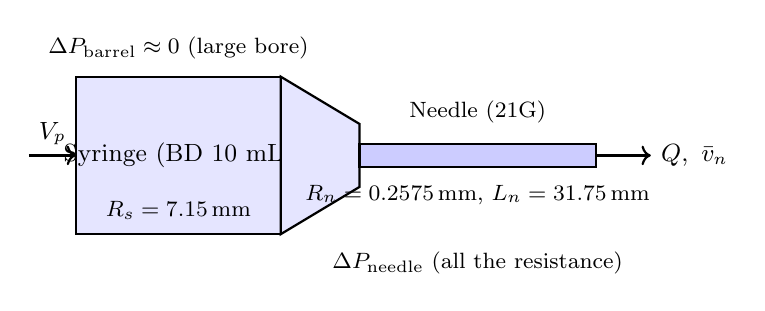
\begin{tikzpicture}[every node/.style={font=\small}]
  % Syringe barrel
  \draw[thick, fill=blue!10] (0,0) rectangle (2.6,2.0);
  \draw[->,thick] (-0.6,1.0) -- (0.0,1.0) node[midway,above]{$V_p$};
  \node at (1.3,1.0) {Syringe (BD 10 mL)};
  \node at (1.3,0.3) {\footnotesize $R_s = 7.15$\,mm};
  % Cone
  \draw[thick, fill=blue!10] (2.6,2.0) -- (3.6,1.4) -- (3.6,0.6) -- (2.6,0.0) -- cycle;
  % Needle
  \draw[thick,fill=blue!20] (3.6,0.85) rectangle (6.6,1.15);
  \node at (5.1,1.55) {\footnotesize Needle (21G)};
  \node at (5.1,0.5) {\footnotesize $R_n = 0.2575$\,mm, $L_n = 31.75$\,mm};
  % Exit
  \draw[->,thick] (6.6,1.0) -- (7.3,1.0) node[right]{$Q,\ \bar v_n$};
  % Labels
  \node[above] at (1.3,2.1) {\footnotesize $\Delta P_\mathrm{barrel}\approx 0$ (large bore)};
  \node[below] at (5.1,-0.1) {\footnotesize $\Delta P_\mathrm{needle}$ (all the resistance)};
\end{tikzpicture}
\caption{The DIW hydraulic loop. The operator commands $V_p$; syringe
geometry fixes $Q$; the ink rheology and needle geometry fix $\tau_w$
and $\Delta P$. The syringe barrel contributes negligible pressure drop
because $(R_s/R_n)^4\approx 5\times 10^5$ -- almost all resistance is
in the needle.}
\label{fig:loop}
\end{figure}

\subsection{Mass balance: from $V_p$ to flow}
\label{sec:mass_balance_Q}

\emph{Motivation.}
If you skip this step and guess $Q$ from the slicer's extrusion rate
setting (which presumes FFF-style filament diameter, not a piston), you
will be off by a factor of $\sim 10^3$. The calculation is two lines of
algebra -- there is no excuse for guessing.

The piston advances at $V_p$, displacing fluid at volumetric rate
\begin{equation}
Q \;=\; \pi R_s^2 \, V_p.
\label{eq:Q_from_Vp}
\end{equation}
The same $Q$ passes through the needle (continuity):
\begin{equation}
\bar v_n \;=\; \frac{Q}{\pi R_n^2}
           \;=\; \left(\frac{R_s}{R_n}\right)^2 V_p.
\label{eq:vbar_n}
\end{equation}
For our hardware ($R_s=7.15$\,mm, 21G $R_n=0.2575$\,mm), the area ratio
$(R_s/R_n)^2\approx 771$. \textbf{A 1\,\si{\mm/\s} piston velocity
becomes a 771\,\si{\mm/\s} mean needle velocity.}

\begin{derivationbox}[title={DERIVATION --- Mass balance: $V_p\to Q\to\bar v_n$}]
\textbf{Assumptions.}
(i)~The ink is incompressible ($\rho=\mathrm{const}$).
(ii)~Piston sealing is perfect ($f_\mathrm{slip}=1$; relaxed in
Ch.~\ref{sec:flow_factor}).
(iii)~The barrel diameter is uniform over the piston stroke
($A_\mathrm{piston}=\mathrm{const}$).

\medskip\noindent\textbf{Step 1 -- Volumetric flow from the piston.}

In time $\mathrm{d}t$ the piston face advances by $V_p\,\mathrm{d}t$,
sweeping a volume $\mathrm{d}\mathcal{V}=A_\mathrm{piston}\,V_p\,\mathrm{d}t$.
Because the fluid is incompressible and the barrel walls do not move, the
same volume must leave through the needle exit per unit time:
\begin{equation}
Q \;=\; \frac{\mathrm{d}\mathcal{V}}{\mathrm{d}t}
  \;=\; A_\mathrm{piston}\,V_p
  \;=\; \frac{\pi D_\mathrm{syringe}^2}{4}\,V_p
  \;=\; \pi R_s^2\,V_p.
\tag{\ref{eq:Q_from_Vp} restated}
\end{equation}

\noindent\textbf{Step 2 -- Mean needle velocity by continuity.}

Continuity for steady, incompressible, one-dimensional flow between any two
cross-sections $i$ and $j$ requires $A_i\bar v_i = A_j\bar v_j = Q$.
Applying this between the piston face (cross-section $s$, area
$A_s=\pi R_s^2$, velocity $V_p$) and the needle interior (cross-section
$n$, area $A_n=\pi R_n^2$, mean velocity $\bar v_n$):
\begin{equation}
A_s\,V_p \;=\; A_n\,\bar v_n
\quad\Longrightarrow\quad
\bar v_n \;=\; \frac{A_s}{A_n}\,V_p
             \;=\; \frac{\pi R_s^2}{\pi R_n^2}\,V_p
             \;=\; \left(\frac{R_s}{R_n}\right)^2\!V_p.
\tag{\ref{eq:vbar_n} restated}
\end{equation}

\noindent\textbf{Step 3 -- Hardware numbers (BD 10\,mL + 21G).}

\begin{itemize}[leftmargin=1.6em,itemsep=1pt]
  \item Syringe: $D_\mathrm{syringe}=\SI{14.3}{\mm}$,
    so $R_s=\SI{7.15}{\mm}$,
    $A_s=\pi(7.15)^2\approx\SI{160.7}{\mm^2}$.
  \item 21G needle: $D_\mathrm{needle}=\SI{0.515}{\mm}$,
    so $R_n=\SI{0.2575}{\mm}$,
    $A_n=\pi(0.2575)^2\approx\SI{0.2083}{\mm^2}$.
  \item Area ratio: $A_s/A_n = 160.7/0.2083 \approx 771$.
\end{itemize}

Therefore:
\begin{equation}
\bar v_n \;=\; 771\,V_p.
\label{eq:vbar_21G}
\end{equation}
At $V_p=\SI{0.01}{\mm/\s}$: $\bar v_n = 771\times 0.01 =
\SI{7.71}{\mm/\s}$; $Q=160.7\times 0.01=\SI{1.607}{\mm^3/\s}=
\SI{96.4}{\micro\liter/\min}$.

For 22G ($D_\mathrm{needle}=\SI{0.413}{\mm}$, $R_n=\SI{0.2065}{\mm}$,
$A_n=\pi(0.2065)^2\approx\SI{0.1340}{\mm^2}$):
$A_s/A_n\approx 1199$, so $\bar v_n\approx 1199\,V_p$.

\medskip\noindent\textbf{Key insight.} $V_p$ is the operator's lever; $\bar
v_n$ and $Q$ follow deterministically from geometry alone -- no
rheological input needed at this stage.
\end{derivationbox}

\subsection{Velocity profile inside the needle}
\label{sec:velocity_profile}

\emph{Motivation.}
Knowing the \emph{mean} needle velocity $\bar v_n$ is not enough for
cell-safety evaluation: a cell suspended near the needle wall experiences
a local shear rate that may be ten to a hundred times the tube average.
The velocity profile shape -- controlled by the Bingham number -- tells you
whether your cells spend the transit in a low-shear core (plug flow,
high $\Bi$) or are exposed to full parabolic shear (Newtonian limit, low
$\Bi$). Getting this wrong means under- or over-estimating cell damage.

The shape of the velocity profile inside the needle depends on the Bingham
number. Figure~\ref{fig:profiles} shows the two limits.

\begin{figure}[h]
\centering
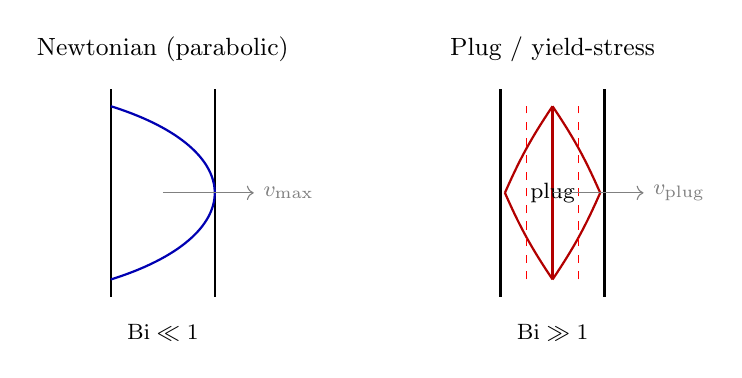
\begin{tikzpicture}[scale=1.1, every node/.style={font=\footnotesize}]
  % ---- Newtonian (parabolic) ----
  \begin{scope}[xshift=0cm]
    \draw[thick] (-0.6,-1.2) -- (-0.6,1.2);
    \draw[thick] (0.6,-1.2) -- (0.6,1.2);
    \node[above] at (0,1.4) {\small Newtonian (parabolic)};
    % Parabola via bezier
    \draw[blue!70!black,thick]
      (-0.6,-1.0) .. controls (1.0,-0.5) and (1.0,0.5) .. (-0.6,1.0);
    \draw[->,thin,gray] (0,0) -- (1.05,0) node[right]{$v_\mathrm{max}$};
    \node[below] at (0,-1.4) {$\Bi\ll 1$};
  \end{scope}
  % ---- Plug flow ----
  \begin{scope}[xshift=4.5cm]
    \draw[thick] (-0.6,-1.2) -- (-0.6,1.2);
    \draw[thick] (0.6,-1.2) -- (0.6,1.2);
    \node[above] at (0,1.4) {\small Plug / yield-stress};
    \draw[red!70!black,thick] (0,-1.0) -- (0,1.0);
    \draw[red!70!black,thick] (0,1.0) to[bend right=5] (-0.55,0);
    \draw[red!70!black,thick] (0,-1.0) to[bend left=5] (-0.55,0);
    \draw[red!70!black,thick] (0,1.0) to[bend left=5] (0.55,0);
    \draw[red!70!black,thick] (0,-1.0) to[bend right=5] (0.55,0);
    \draw[red,dashed,thin] (-0.3,-1.0) -- (-0.3,1.0);
    \draw[red,dashed,thin] (0.3,-1.0) -- (0.3,1.0);
    \node at (0,0) {plug};
    \draw[->,thin,gray] (0,0) -- (1.05,0) node[right]{$v_\mathrm{plug}$};
    \node[below] at (0,-1.4) {$\Bi\gg 1$};
  \end{scope}
\end{tikzpicture}
\caption{Velocity profiles in the needle cross-section.
Left: Newtonian / power-law fluid -- maximum shear at the wall, zero at
the centreline. Right: plug-flow limit for a high-yield-stress fluid --
most of the cross-section moves as a solid plug; shear is concentrated
in thin wall layers. Our CMC inks lie between these limits; high-modulus
inks (Bozano) approach the plug-flow regime.}
\label{fig:profiles}
\end{figure}

\paragraph{Biological significance.} Cells suspended in the ink
experience the \emph{local} shear rate, not the wall average. In
plug flow, cells in the core see very low shear stress. For
bioprinting with live cells, inks with partial plug-flow behaviour
(high $\Bi$) are preferable because the cell-damaging high-shear zone
is confined to a thin wall layer.

\subsection{Mass balance: from $V_p$ to print speed}
\label{sec:mass_balance_vprint}

\emph{Motivation.}
If you set $V_p$ and $v_\mathrm{print}$ independently -- the classic
error of separating ``extrusion speed'' from ``travel speed'' -- you
will either over-extrude (swell, clogged layers) or under-extrude (broken
filaments). The relationship is not a tuning knob; it is a consequence of
volume conservation, and it fixes the ratio $v_\mathrm{print}/V_p$ from
geometry alone.

The print head deposits a filament of cross-section $w\,h_\mathrm{layer}$
as it moves over the build plate at speed $v_\mathrm{print}$:
\begin{equation}
Q \;=\; v_\mathrm{print}\, w\, h_\mathrm{layer}.
\label{eq:vprint}
\end{equation}
With $w\approx 2R_n(1+\beta_\mathrm{swell})$ and
$h_\mathrm{layer}=h_\mathrm{factor}\cdot 2R_n$ this becomes
\begin{equation}
v_\mathrm{print}
\;\approx\;
\frac{\pi(R_s/R_n)^2}{4\,h_\mathrm{factor}(1+\beta_\mathrm{swell})}\,V_p
\;\approx\; \frac{700\text{--}865}{(1+\beta_\mathrm{swell})}\,V_p
\qquad\text{(21G)}.
\label{eq:vprint_Vp}
\end{equation}

\begin{derivationbox}[title={DERIVATION --- Volume conservation: $V_p\to v_\mathrm{print}$}]
\textbf{Assumptions.}
(i)~Incompressible ink ($f_\mathrm{slip}=1$, $k_\mathrm{flow}=1$;
corrections deferred to Ch.~\ref{sec:flow_factor}).
(ii)~The deposited filament cross-section is a rectangle of width $w$ and
height $h_\mathrm{layer}$ (rounded cross-sections are accommodated by
adjusting $h_\mathrm{factor}$).
(iii)~No voids, no over-compression: volume extruded equals volume
deposited.

\medskip\noindent\textbf{Step 1 -- Equate extruded and deposited volume
rates.}

The extruded volumetric rate is $Q = \pi R_s^2 V_p$ (from
Eq.~\ref{eq:Q_from_Vp}).
The deposited volumetric rate equals the deposited cross-sectional area
swept by the print head:
\begin{equation}
Q \;=\; v_\mathrm{print}\,A_\mathrm{bead}, \qquad
A_\mathrm{bead} \;=\; w\,h_\mathrm{layer}.
\label{eq:vol_cons_bead}
\end{equation}

\noindent\textbf{Step 2 -- Parameterise the bead geometry.}

The filament width is set by the needle exit diameter, amplified by die
swell:
\begin{equation}
w \;=\; 2R_n\,(1+\beta_\mathrm{swell}) \;=\; D_\mathrm{needle}(1+\beta_\mathrm{swell}).
\label{eq:bead_width}
\end{equation}
The layer height is a controlled fraction of the needle diameter (typical
$h_\mathrm{factor}\approx 0.7$--$1.0$ in DIW):
\begin{equation}
h_\mathrm{layer} \;=\; h_\mathrm{factor}\cdot 2R_n.
\label{eq:bead_height}
\end{equation}

\noindent\textbf{Step 3 -- Solve for $v_\mathrm{print}$.}

Substituting Eqs.~\ref{eq:bead_width}--\ref{eq:bead_height} into
Eq.~\ref{eq:vol_cons_bead} and using $Q=\pi R_s^2 V_p$:
\begin{align}
v_\mathrm{print}
  &\;=\; \frac{Q}{w\,h_\mathrm{layer}}
   \;=\; \frac{\pi R_s^2\,V_p}
              {2R_n(1+\beta_\mathrm{swell})\cdot h_\mathrm{factor}\cdot 2R_n}
\nonumber\\[4pt]
  &\;=\; \frac{\pi R_s^2}
              {4\,R_n^2\,h_\mathrm{factor}(1+\beta_\mathrm{swell})}\,V_p
   \;=\; \frac{\pi (R_s/R_n)^2}
              {4\,h_\mathrm{factor}(1+\beta_\mathrm{swell})}\,V_p.
\label{eq:vprint_derived}
\end{align}

\noindent\textbf{Step 4 -- Hardware numbers (21G, $\beta_\mathrm{swell}=0$).}

$(R_s/R_n)^2 \approx 771$; $h_\mathrm{factor}\in[0.7, 1.0]$:
\begin{equation*}
v_\mathrm{print}
\;=\; \frac{\pi\cdot 771}{4\,h_\mathrm{factor}}\,V_p
\;\approx\; \frac{606}{h_\mathrm{factor}}\,V_p
\;\in\; [606, 865]\,V_p,
\end{equation*}
recovering Eq.~\ref{eq:vprint_Vp}. The range $700$--$865$ in the main
text corresponds to $h_\mathrm{factor}\approx 0.87$--$0.70$
(a larger layer height gives a lower print speed for the same flow).

\medskip\noindent\textbf{Physical check.} Dimensional consistency:
$[v_\mathrm{print}] = [\pi(R_s/R_n)^2\,V_p / (4\,h_\mathrm{factor})]$
= (dimensionless)(mm/s) = \si{\mm/\s}. \checkmark
\end{derivationbox}

\begin{intuitionbox}
\textbf{The piston is the slowest thing.} On 21G, $V_p$ in \si{\mm/\s}
maps to $v_\mathrm{print}$ in \si{\mm/\s} with a multiplier of
$\approx 700$--$865$:
\begin{itemize}[leftmargin=1.4em,itemsep=1pt]
\item $V_p=0.005 \Rightarrow v_\mathrm{print}\approx 4\,\mms$
\item $V_p=0.010 \Rightarrow v_\mathrm{print}\approx 8\,\mms$
\item $V_p=0.030 \Rightarrow v_\mathrm{print}\approx 25\,\mms$
\item $V_p=0.050 \Rightarrow v_\mathrm{print}\approx 40\,\mms$
\end{itemize}
The mechanical envelope of the lab gantry is roughly
$v_\mathrm{print}\in[3,30]\,\mms$, so $V_p\in[\sim 0.004,\sim 0.04]\,\mms$.
\end{intuitionbox}

\begin{dimensionlessbox}
\textbf{Generalised Reynolds number} for power-law flow in a tube:
\begin{equation}
\Rey_\mathrm{gen} \;=\;
\frac{\rho\,\bar v_n^{2-n}\,(2R_n)^n}{K\,8^{n-1}}
\left(\frac{4n}{3n+1}\right)^n.
\end{equation}
For laminar flow (the fundamental assumption of all our $\Delta P$
equations), $\Rey_\mathrm{gen}\ll 2100$. For our operating conditions:

\medskip\centering
\begin{tabular}{lcc}
\toprule
Ink (PL fit) & $K$ [\si{\Pa\s^n}] & $\Rey_\mathrm{gen}$ at $V_p=0.01\,\mms$ \\
\midrule
C15           & 78   & $\ll 1$ (deeply laminar) \\
C15 Gira 5.5  & 267  & $\ll 1$ \\
Bozano        & 1086 & $\ll 1$ \\
\bottomrule
\end{tabular}
\medskip\flushleft
All three inks are deeply laminar across the entire printable $V_p$
range. The fully-developed laminar flow assumption is valid. No
turbulence correction is needed.
\end{dimensionlessbox}

% ---- Metzner--Reed derivation ----------------------------------------
\begin{derivationbox}[title={DERIVATION --- Generalised (Metzner--Reed) Reynolds number}]
\label{box:metzner_reed}

\textbf{Context.}
The classical Hagen--Poiseuille and Stokes formulae were derived for
Newtonian fluids; the Reynolds number $\Rey=\rho\bar v D/\eta$ uses a
single, constant viscosity. For a power-law fluid the apparent viscosity
depends on shear rate, so ``which $\eta$ to use?'' is ill-defined.
\citet{MetznerReed1955} resolved this by constructing a Reynolds number
whose laminar-to-turbulent threshold remains at $\Rey_\mathrm{gen}\approx 2100$
regardless of the flow index $n$, provided the correct generalised
denominator is used.

\medskip
\noindent\textbf{Step 1 -- Laminar wall shear rate for a power-law fluid.}

For steady, fully developed, laminar flow of a power-law fluid
($\tau=K\gd^n$) in a tube of radius $R$, integration of the velocity
profile gives the Newtonian wall shear rate corrected by the
Rabinowitsch--Weissenberg factor:
\begin{equation}
\gd_w \;=\; \frac{4\bar v}{R_n}
            \cdot\frac{3n+1}{4n}
           \;=\; \frac{8\bar v}{D}
            \cdot\frac{3n+1}{4n},
\label{eq:gdw_PL}
\end{equation}
where $D=2R_n$ is the tube diameter and $\bar v \equiv \bar v_n$ is the
cross-sectional mean velocity. The factor $(3n+1)/4n$ corrects for the
non-parabolic profile: for $n=1$ (Newtonian) it equals 1, recovering the
classical Newtonian result $\gd_w=8\bar v/D$; for $n<1$ (shear thinning)
it is greater than 1, reflecting the steeper gradient near the wall.

\medskip
\noindent\textbf{Step 2 -- Wall shear stress in terms of $\bar v$.}

Substituting Eq.~\ref{eq:gdw_PL} into the power-law constitutive equation
$\tau_w = K\gd_w^n$:
\begin{align}
\tau_w
  &\;=\; K\!\left[\frac{8\bar v}{D}
         \cdot\frac{3n+1}{4n}\right]^{\!n}
\nonumber\\
  &\;=\; K\!\left(\frac{8\bar v}{D}\right)^{\!n}
         \!\left(\frac{3n+1}{4n}\right)^{\!n}.
\label{eq:tau_w_PL_vbar}
\end{align}
This may be rewritten in the Metzner--Reed form by introducing the
\emph{generalised viscosity} $\mu'$:
\begin{equation}
\tau_w \;=\; \mu'\!\left(\frac{8\bar v}{D}\right),
\qquad
\mu' \;=\; K\!\left(\frac{8\bar v}{D}\right)^{\!n-1}
            \left(\frac{3n+1}{4n}\right)^{\!n}.
\label{eq:mu_prime}
\end{equation}

\medskip
\noindent\textbf{Step 3 -- Construct $\Rey_\mathrm{gen}$ by analogy with
the Newtonian case.}

For a Newtonian fluid, $\tau_w = \eta\cdot(8\bar v/D)$, and the Reynolds
number is $\Rey = \rho\bar v D/\eta$. By dimensional analogy, replace
$\eta$ with $\mu'$:
\begin{equation}
\Rey_\mathrm{gen}
\;=\; \frac{\rho\,\bar v_n\,D}{\mu'}
\;=\; \frac{\rho\,\bar v_n\,D}
           {K\!\left(\dfrac{8\bar v_n}{D}\right)^{\!n-1}\!\left(\dfrac{3n+1}{4n}\right)^{\!n}}.
\label{eq:Re_gen_step3}
\end{equation}

\medskip
\noindent\textbf{Step 4 -- Simplify to the standard form.}

Collect powers of $\bar v_n$ and $D$ in the denominator:
$(8\bar v_n/D)^{n-1} = 8^{n-1}\bar v_n^{n-1}/D^{n-1}$. Then:
\begin{align}
\Rey_\mathrm{gen}
  &\;=\; \frac{\rho\,\bar v_n\,D}
              {K\cdot 8^{n-1}\,\bar v_n^{n-1}\,D^{-(n-1)}
               \cdot\left(\frac{3n+1}{4n}\right)^{\!n}}
\nonumber\\
  &\;=\; \frac{\rho\,\bar v_n^{1-(n-1)}\,D^{1+(n-1)}}
              {K\cdot 8^{n-1}\left(\frac{3n+1}{4n}\right)^{\!n}}
\nonumber\\
  &\;=\; \frac{\rho\,\bar v_n^{2-n}\,D^{\,n}}
              {K\,8^{n-1}\left(\frac{3n+1}{4n}\right)^{\!n}}.
\label{eq:re_gen_step}
\end{align}

Using $D=2R_n$ and noting $\left(\frac{4n}{3n+1}\right)^n =
1/\left(\frac{3n+1}{4n}\right)^n$:
\begin{equation}
\boxed{
\Rey_\mathrm{gen}\;=\;
\frac{\rho\,\bar v_n^{\,2-n}\,(2R_n)^{\,n}}
{K\,8^{\,n-1}\!\left(\dfrac{3n+1}{4n}\right)^{\!n}}
\;=\;
\frac{\rho\,\bar v_n^{\,2-n}\,D^{\,n}}
{K\,8^{\,n-1}}\left(\frac{4n}{3n+1}\right)^{\!n}.
}
\label{eq:re_gen}
\end{equation}

This is the Metzner--Reed generalised Reynolds number \citep{MetznerReed1955}.
For Newtonian flow ($n=1$, $K=\eta$) it reduces exactly to
$\Rey=\rho\bar v D/\eta$. The laminar criterion is
$\Rey_\mathrm{gen}\lesssim 2100$; turbulent transition occurs above
$\Rey_\mathrm{gen}\approx 3000$--$4000$ for power-law fluids.

\medskip
\noindent\textbf{Step 5 -- Qualitative evaluation for our inks.}

For the three inks in this project, the key parameters are $n<0.5$ (strong
shear thinning) and $K\gg 1\,\si{\Pa\s^n}$ (high consistency). The
operating needle diameter is $D\sim\SI{0.5}{\mm}$ and the mean needle
velocity (from Eq.~\ref{eq:vbar_21G}) at $V_p=\SI{0.01}{\mm/\s}$ is
$\bar v_n \approx \SI{7.7}{\mm/\s}=\SI{7.7e-3}{\m/\s}$.
Taking $\rho\approx\SI{1000}{\kg/\m^3}$ (water-based ink),
$n=0.3$, $K=\SI{100}{\Pa\s^n}$:

\begin{align*}
8^{n-1} &= 8^{-0.7} \approx 0.233, \\
\left(\frac{3(0.3)+1}{4(0.3)}\right)^{0.3}
  &= \left(\frac{1.9}{1.2}\right)^{0.3}
   = (1.583)^{0.3} \approx 1.148, \\
\bar v_n^{2-n} &= (7.71\times10^{-3})^{1.7}
   \approx 2.56\times10^{-4}\,\si{\m^{1.7}/\s^{1.7}}, \\
D^n &= (5.15\times10^{-4})^{0.3}
  \approx 0.103\,\si{\m^{0.3}}, \\
\Rey_\mathrm{gen}
  &= \frac{1000\cdot 2.56\times10^{-4}\cdot 0.103}
          {100\cdot 0.233 \cdot 1.148}
   \approx \frac{2.64\times10^{-2}}{26.7}
   \approx 9.8\times10^{-4}.
\end{align*}

$\Rey_\mathrm{gen}\approx 9.8\times10^{-4}\approx 10^{-3}\ll 1 \ll 2100$: the flow is
\textbf{deeply laminar} by more than three orders of magnitude. This
confirms that every analytical velocity-profile result in this book --
the Hagen--Poiseuille pressure formulae, the Rabinowitsch integral,
the wall-shear-stress expressions -- rests on solid ground for all three
inks across the entire printable $V_p$ range.
\end{derivationbox}

\begin{inpracticebox}
\textbf{Pre-print flow-regime check (takes $<$5 minutes).}
Before loading any new ink or switching needle gauge, compute two
dimensionless numbers:
\begin{enumerate}[leftmargin=1.6em,itemsep=3pt]
  \item \textbf{$\Rey_\mathrm{gen}$ (Eq.~\ref{eq:re_gen}):}
    use the Power-Law $K$ and $n$ from \texttt{Fit\_Muitos\_Modelos\_v4.py},
    $\bar v_n$ from Eq.~\ref{eq:vbar_21G} at your target $V_p$, and
    $\rho\approx\SI{1000}{\kg/\m^3}$ for water-based inks. If
    $\Rey_\mathrm{gen}<1$, all pressure formulae are valid. If it
    approaches 100, add a note in your lab record.

  \item \textbf{$\Bi$ (Bingham number):}
    use $\tau_y \approx G'_\mathrm{LVR}\,\gamma_\mathrm{LVR}$
    (Eq.~\ref{eq:yield_proxy}) and estimate $\eta_p \approx \eta_\infty$
    from the Cross fit. If $\Bi>1$, expect a partial plug at the centre --
    plan for the cell-viability benefit and check that the plug radius
    does not cause clogging at the needle entrance.
\end{enumerate}
\textbf{Rule:} If $\Rey_\mathrm{gen}<1$ \emph{and} $\Bi>1$, the ink is in
the preferred bioprinting regime: analytically tractable laminar flow with
a low-shear cell-protective core. Record both numbers in the print log
alongside $V_p$ and needle gauge.
\end{inpracticebox}

\begin{goingdeeperbox}
\textbf{Why the $8^{n-1}$ and $((3n+1)/4n)^n$ factors?}
Both arise from the Rabinowitsch correction to the Newtonian wall-shear-rate
formula $\gd_w^\mathrm{N}=8\bar v/D$. For a general generalised Newtonian
fluid the true wall shear rate is
$\gd_w = \gd_w^\mathrm{N}\cdot\tfrac{3n'+1}{4n'}$, where $n'=
\mathrm{d}\log\tau_w/\mathrm{d}\log(8\bar v/D)$ is the local log-log slope
of the flow curve. For a power-law fluid $n'=n$ is constant, giving the
exact result used in Step~1. For a Cross fluid $n'$ varies with $\bar v$,
and the Rabinowitsch correction must be applied numerically via the integral
in Eq.~\ref{eq:rabinowitsch}. The Metzner--Reed group then becomes an
\emph{effective} Reynolds number; its laminar threshold still lies near 2100
for most generalised Newtonian models, making it the universal laminar-flow
diagnostic in non-Newtonian pipe flow \citep{MetznerReed1955}.
\end{goingdeeperbox}

% ---- Exercises --------------------------------------------------------
\subsection*{Check Yourself}
\label{sec:hydraulic_exercises}

\begin{exercise}{\diffA}
At $V_p=\SI{0.010}{\mm/\s}$ on a 21G needle (inner radius
$R_n=\SI{0.2575}{\mm}$, syringe inner radius $R_s=\SI{7.15}{\mm}$):
\begin{enumerate}[label=(\alph*),leftmargin=1.6em,itemsep=1pt]
  \item Compute the volumetric flow $Q$ in \si{\mm^3/\s} and
    \si{\micro\liter/\min}.
  \item Compute the mean needle velocity $\bar v_n$ in \si{\mm/\s}.
  \item Repeat (b) for a 22G needle ($R_n=\SI{0.2065}{\mm}$).
\end{enumerate}
\begin{solution}
(a) $Q = \pi R_s^2 V_p = \pi(7.15)^2(0.010)
       = \pi(51.12)(0.010) \approx \SI{1.607}{\mm^3/\s}
       = 1.607\times60 \approx \SI{96.4}{\micro\liter/\min}$.

(b) $\bar v_n = (R_s/R_n)^2 V_p = (7.15/0.2575)^2 \times 0.010
              = (27.77)^2 \times 0.010 = 771.2 \times 0.010
              \approx \SI{7.71}{\mm/\s}$.

(c) $(R_s/R_n)^2 = (7.15/0.2065)^2 = (34.63)^2 = 1199.2$;
    $\bar v_n = 1199.2 \times 0.010 \approx \SI{12.0}{\mm/\s}$.

Note: switching from 21G to 22G at the same $V_p$ raises $\bar v_n$
by a factor of $1199/771\approx 1.56$ and raises $\Delta P$ by roughly
$(R_\mathrm{21G}/R_\mathrm{22G})^4 = (0.2575/0.2065)^4 \approx 2.4$.
\end{solution}
\end{exercise}

\begin{exercise}{\diffB}
For an ink with Power-Law parameters $K=\SI{100}{\Pa\s^n}$, $n=0.30$,
density $\rho=\SI{1000}{\kg/\m^3}$, printed through a 21G needle
($D=\SI{0.515}{\mm}=\SI{5.15e-4}{\m}$) at $V_p=\SI{0.01}{\mm/\s}$:
\begin{enumerate}[label=(\alph*),leftmargin=1.6em,itemsep=1pt]
  \item Compute $\bar v_n$ in \si{\m/\s}.
  \item Evaluate each factor in Eq.~\ref{eq:re_gen} explicitly.
  \item State whether fully-developed laminar flow is a valid assumption.
\end{enumerate}
\textit{(Use the assumed round values given in the stem; do not substitute
fitted parameters from the appendices.)}
\begin{solution}
(a) $\bar v_n = 771\times 0.010 = \SI{7.71}{\mm/\s} = \SI{7.71e-3}{\m/\s}$.

(b) Factor-by-factor:
\begin{align*}
\rho\,\bar v_n^{2-n}
  &= 1000\times(7.71\times10^{-3})^{1.70}
   = 1000\times 2.56\times10^{-4}
   = 0.256\;\si{\kg\m^{n-3}\s^{n-2}},\\
D^n &= (5.15\times10^{-4})^{0.30}
     = e^{0.30\ln(5.15\times10^{-4})}
     = e^{0.30\times(-7.571)}
     = e^{-2.271} \approx 0.103\;\si{\m^n},\\
\text{numerator} &= 0.256\times0.103 \approx 2.64\times10^{-2},\\[4pt]
8^{n-1} &= 8^{-0.70} = e^{-0.70\ln 8} = e^{-1.456} \approx 0.233,\\
\left(\frac{3n+1}{4n}\right)^n
  &= \left(\frac{1.90}{1.20}\right)^{0.30}
   = (1.583)^{0.30}
   = e^{0.30\times0.460}
   = e^{0.138} \approx 1.148,\\
\text{denominator} &= 100\times0.233\times1.148 \approx 26.7,\\[4pt]
\Rey_\mathrm{gen}
  &= 2.64\times10^{-2}/26.7 \approx 9.8\times10^{-4}.
\end{align*}

(c) $\Rey_\mathrm{gen}\approx 9.8\times10^{-4}\ll 1\ll 2100$: the flow is
deeply laminar. Fully-developed laminar flow is an excellent assumption;
no turbulence correction is needed and the analytical $\Delta P$ formulae
are valid.
\end{solution}
\end{exercise}

\begin{exercise}{\diffC}
A cell-loaded ink has a Bingham number $\Bi=12$ at the wall shear rate
imposed by a 21G needle at the nominal print speed.
\begin{enumerate}[label=(\alph*),leftmargin=1.6em,itemsep=1pt]
  \item Sketch the expected velocity profile qualitatively. What fraction
    of the cross-sectional area is occupied by the plug (unyielded core)?
    The plug radius for a Bingham fluid is $r_\mathrm{plug}=
    R_n\cdot\tau_y/\tau_w$; express this as a fraction of $R_n$ in
    terms of $\Bi$ for $\Bi\gg 1$.
  \item What does a high $\Bi$ imply about the shear rate that cells in
    the core of the needle experience? Relate this to cell viability
    literature ($\tau_w<\SI{5}{\kPa}$ for human cells).
  \item If you switch to a 22G needle at the same $V_p$, qualitatively
    how does $\Bi$ change, and is the change beneficial or detrimental
    for cell viability? (Hint: $\tau_w$ scales as $R_n^{-(3+n)}$ for a
    power-law fluid at fixed $V_p$; $\gd_w$ scales as $R_n^{-3}$.)
\end{enumerate}
\begin{solution}
(a) The plug radius is $r_\mathrm{plug}/R_n = \tau_y/\tau_w$. By
definition $\Bi=\tau_y/(\eta_p\,\gd_w)$ and $\tau_w=\tau_y+\eta_p\gd_w$,
so for the Bingham model $\tau_w/\tau_y = 1+1/\Bi$. Therefore
$r_\mathrm{plug}/R_n = \tau_y/\tau_w = 1/(1+1/\Bi) = \Bi/(\Bi+1)$.
At $\Bi=12$: $r_\mathrm{plug}/R_n = 12/13\approx 0.923$.
The plug occupies $(r_\mathrm{plug}/R_n)^2\approx 0.85$ -- about 85\%
of the cross-sectional area. The velocity profile shows a broad flat
plug with thin shear layers of thickness $\sim0.077\,R_n$ at the wall.

(b) In the plug, $\gd=0$: cells in the core experience zero shear rate
and zero shear stress during transit. Only cells within the thin wall
layer are exposed to high shear. For $\Bi=12$, 85\% of the cells are
in zero-shear conditions; only the outer 15\% of the \emph{area}
(but a thin annulus) experiences wall-level shear. The cell-safety
criterion $\tau_w<\SI{5}{\kPa}$ still applies to the wall annulus, but
the \emph{majority} of cells are well-protected. This is why high-$\Bi$
inks are preferred for cell-loaded bioprinting.

(c) Switching 21G $\to$ 22G at fixed $V_p$: $R_n$ decreases
($0.2575\to\SI{0.2065}{\mm}$), so $\gd_w\propto R_n^{-3}$ increases,
and $\tau_w\propto R_n^{-(3+n)}$ increases even faster (for $n=0.3$:
factor $(0.2575/0.2065)^{3.3}\approx 2.0$ increase in $\tau_w$, but
$\tau_y$ is unchanged). Therefore $\Bi=\tau_y/(\eta_p\gd_w)$ decreases:
the ink is less plug-like in 22G than in 21G at the same $V_p$.
The change is \textbf{detrimental} for cell viability: the protective
plug shrinks (lower $\Bi$) \emph{and} the absolute wall stress increases.
For cell-loaded prints, the 21G is the preferred gauge unless resolution
requirements demand 22G.
\end{solution}
\end{exercise}

\begin{runningbox}{RUNNING EXAMPLE -- Solution to Q2}
\textbf{Question.} What piston velocity $V_p$ should Ana command?

\medskip\textbf{Reasoning.} The mechanical envelope is
$v_\mathrm{print}\in[3,30]\,\mms$. Ana picks a target of
$v_\mathrm{print}\approx 8\,\mms$ -- slow enough to forgive minor
mis-calibration, fast enough to finish the production print in under
an hour.

For 21G with $\beta_\mathrm{swell}\approx 0$ (justified for the NE,
see Q4), Eq.~\ref{eq:vprint_Vp} gives amplification $\approx 865$:
\[
V_p \;=\; \frac{8}{865} \;\approx\; 0.0093\,\mms
\;\to\; \text{rounded to } \mathbf{0.01\,\mms}.
\]

\textbf{Sanity check.} $Q=\pi(7.15)^2\cdot 0.01=1.6\,\si{\mm^3/\s}
\approx 100\,\si{\mu L/min}$ -- typical for syringe bioprinting.

\medskip\emph{Still unknown:} is the resulting $\Delta P$ within
hardware limits? Q3.
\end{runningbox}

\begin{takeawaybox}
\begin{itemize}[leftmargin=1.4em,itemsep=2pt]
\item \textbf{$V_p$ is the only setpoint.} $\Delta P$, $Q$, $\bar v_n$,
  $\tau_w$, and $v_\mathrm{print}$ are all consequences of $V_p$ plus
  geometry. Treating $\Delta P$ as a control input is the classic DIW
  error.
\item $V_p\to Q\to\bar v_n$: a factor of $\sim 771$ velocity
  amplification on 21G. The piston is slow; the needle is fast.
\item $v_\mathrm{print}$ is set by $V_p$ and geometry alone -- it is not
  an independent knob unless the slicer X/Y feedrate is decoupled from E.
\item The Metzner--Reed $\Rey_\mathrm{gen}$ (Eq.~\ref{eq:re_gen})
  generalises the Newtonian Reynolds number for power-law fluids; its
  laminar threshold is still $\approx 2100$.
  $\Rey_\mathrm{gen}\ll 2100$ for all printable conditions: laminar
  flow is always valid, and every analytical $\Delta P$ formula in this
  book is sound.
\item Plug flow in high-$\Bi$ inks protects cells in the core from
  damaging shear: $\sim85\%$ of the cross-sectional area is zero-shear
  at $\Bi=12$.
\end{itemize}
\end{takeawaybox}

\begin{designrulebox}
\textbf{DR 3.1.} Always verify $\Rey_\mathrm{gen}\ll 2100$ when changing
needle gauge or ink. Turbulent transition would invalidate all $\Delta P$
and $\tau_w$ calculations. Use Eq.~\ref{eq:re_gen} with the Power-Law
$K$ and $n$ from \texttt{Fit\_Muitos\_Modelos\_v4.py}.

\textbf{DR 3.2.} Do not change needle gauge ($R_n$) without recomputing
all downstream quantities -- the $R_n^{-4}$ scaling of $\Delta P$ makes
gauge changes the largest single-factor lever in the whole workflow.
Switching 21G $\to$ 22G at fixed $V_p$ also raises $\gd_w\propto R_n^{-3}$,
potentially breaching the $\tau_w<\SI{5}{\kPa}$ cell-safety threshold.

\textbf{DR 3.3.} For cell-loaded inks, prefer inks with high $\Bi$
(approaching plug flow) to confine high shear to thin wall layers.
Compute $\Bi$ from the oscillatory yield-stress proxy and the Cross
$\eta_\infty$ before committing to a needle gauge.

\textbf{DR 3.4.} Always compute the $V_p\to v_\mathrm{print}$ ratio
(Eq.~\ref{eq:vprint_Vp}) analytically before entering any print speed
into the slicer. If the slicer decouples travel speed from extrusion,
the extrusion multiplier must absorb the difference.
\end{designrulebox}

% =================================================================
\section{From Flow to Pressure: Hagen--Poiseuille for Non-Newtonian Fluids}
\label{sec:HP}

Given $Q$ from the mass-balance of the previous chapter, we need $\Delta P$
across the needle on two grounds: as a mechanical safety check (does the
required pressure stay inside the syringe rating?) and as the upstream
quantity from which wall shear stress and wall shear rate are derived. Get
$\Delta P$ wrong and you either exceed the syringe burst rating or, worse,
exceed the cell-safe wall-shear ceiling without realising it -- two
independent failure modes from a single mis-predicted number.

\subsection{Newtonian baseline}

\emph{Motivation.} The Newtonian formula sets the physical intuition and the
scaling laws before we extend to non-Newtonian fluids. Every exponent and
denominator in the generalised formulae traces back to this starting point;
understanding the baseline makes the extensions transparent rather than magic.

For a Newtonian fluid in a straight cylinder of radius $R$ and length
$L$, Hagen--Poiseuille gives
\begin{equation}
\Delta P \;=\; \frac{8\,\eta\,L\,Q}{\pi R^4}.
\label{eq:HP_newton}
\end{equation}
The $R^{-4}$ dependence is severe: halving the needle radius multiplies
the pressure 16-fold. This is the dominant reason needle gauge matters
so much.

\begin{intuitionbox}
Think of the $R^{-4}$ scaling in two steps. Halving $R$ doubles the wall
shear rate (the fluid must deform twice as fast in the same time), which
doubles $\tau_w$; and it simultaneously halves the moment arm
$R$ over which that stress acts, so $\Delta P=2L\tau_w/R$ doubles again.
Two doublings give a factor of four -- and that is just the
shear-rate/moment-arm argument. The fourth power includes the $Q\propto
R^2\bar v_n$ reduction in cross-section as well.
\end{intuitionbox}

\subsection{Power-Law extension}

\emph{Motivation.} Our CMC inks are strongly shear-thinning; treating them
as Newtonian at a single representative viscosity can produce $\Delta P$
errors of an order of magnitude. The Power-Law model provides an exact
closed-form correction for any shear-thinning index $n$ -- but only if the
derivation is done rigorously, which is what this subsection supplies.

For a Power-Law fluid, the analytical solution for steady laminar fully-
developed flow in a cylinder gives wall shear stress:
\begin{equation}
\tau_w \;=\; K\!\left(\frac{(3n+1)\,Q}{\pi R^3\, n}\right)^{\!n},
\label{eq:tau_w_PL}
\end{equation}
and pressure drop from a force balance:
\begin{equation}
\Delta P \;=\; \frac{2 L \tau_w}{R}.
\label{eq:HP_PL}
\end{equation}

\begin{derivationbox}[title={DERIVATION --- Power-Law pipe flow: velocity profile, $Q(\tau_w)$, and inversion to $\tau_w(Q)$}]

\textbf{Assumptions.}
(i)~Steady, fully-developed, laminar flow in a straight circular cylinder
of radius $R$ and length $L$.
(ii)~The fluid obeys the Power-Law constitutive model $\tau=K\gd^n$
($n<1$ for shear thinning), with the convention that
$\gd=-dv/dr>0$ for the decreasing velocity profile ($v$ maximal at
the centreline, zero at the wall).
(iii)~No wall slip; no-slip boundary condition $v(R)=0$.
(iv)~Gravity and inertia are negligible (verified by $\Rey_\mathrm{gen}\ll 1$;
see Eq.~\ref{eq:re_gen}).

\medskip\noindent\textbf{Step 1 -- Universal linear stress profile.}

Consider a fluid element in the shape of a coaxial cylinder of radius $r$
($0\leq r\leq R$) and length $L$. In steady flow, Newton's second law
applied to this element along the axial direction balances the net pressure
force on the two end faces against the integrated viscous shear on the
curved surface:
\[
\underbrace{\pi r^2\,\Delta P}_{\text{pressure}} \;=\;
\underbrace{2\pi r\,L\,\tau(r)}_{\text{shear on curved surface}}.
\]
Solving for $\tau(r)$:
\begin{equation}
\tau(r) \;=\; \frac{\Delta P}{2L}\,r.
\label{eq:tau_linear}
\end{equation}
This is a central result: \emph{the shear stress profile is linear in $r$,
regardless of the constitutive model}. It is maximum at the wall
($r=R$):
\begin{equation}
\tau_w \;\equiv\; \tau(R) \;=\; \frac{\Delta P\,R}{2L},
\qquad\Longleftrightarrow\qquad
\Delta P \;=\; \frac{2L\,\tau_w}{R}.
\tag{\ref{eq:HP_PL} derived}
\end{equation}
Only the velocity profile $v(r)$ -- derived in the next step -- depends on
the constitutive model.

\medskip\noindent\textbf{Step 2 -- Velocity profile for a Power-Law fluid.}

Substitute the Power-Law relation into Eq.~\eqref{eq:tau_linear}:
\[
K\!\left(-\frac{dv}{dr}\right)^{\!n} \;=\; \frac{\Delta P}{2L}\,r.
\]
(The sign convention $-dv/dr>0$ makes $\gd>0$ since velocity decreases
toward the wall.) Solving for $-dv/dr$:
\[
-\frac{dv}{dr} \;=\; \left(\frac{\Delta P}{2LK}\right)^{\!1/n} r^{1/n}.
\]
Integrate from $r$ outward to the wall at $R$, applying no-slip $v(R)=0$:
\[
\int_r^R\!\left(-\frac{dv}{dr'}\right)dr' \;=\;
\left(\frac{\Delta P}{2LK}\right)^{\!1/n}
\int_r^R r'^{1/n}\,dr'.
\]
The left side evaluates to $v(R)-v(r)=-v(r)$ (since $v(R)=0$).
The right side integrates as a power of $r'$:
\[
\int_r^R r'^{1/n}\,dr'
\;=\; \left[\frac{r'^{\,1/n+1}}{1/n+1}\right]_r^R
\;=\; \frac{n}{n+1}\Bigl(R^{(n+1)/n}-r^{(n+1)/n}\Bigr).
\]
Substituting back (and reversing the sign on the left):
\begin{equation}
\boxed{v(r) \;=\;
\left(\frac{\Delta P}{2LK}\right)^{\!1/n}
\frac{n}{n+1}
\Bigl(R^{(n+1)/n}-r^{(n+1)/n}\Bigr).}
\label{eq:vr_PL}
\end{equation}
\textit{Sanity checks.} At $r=0$: $v(0)=\left(\Delta P/2LK\right)^{1/n}
\frac{n}{n+1}R^{(n+1)/n}$ -- the centreline maximum. At $r=R$: $v(R)=0$
-- no-slip satisfied. As $n\to 1$ (Newtonian): the profile recovers the
standard parabola $v(r)=(\Delta P/4\eta L)(R^2-r^2)$.
As $n\to 0$: the exponent $(n+1)/n\to\infty$ and the profile becomes
flat -- a ``plug-like'' distribution with all shear concentrated
near the wall.

\medskip\noindent\textbf{Step 3 -- Volumetric flow rate $Q$.}

Integrate $v(r)$ over the circular cross-section:
\[
Q \;=\; \int_0^R v(r)\,2\pi r\,dr
    \;=\; 2\pi\left(\frac{\Delta P}{2LK}\right)^{1/n}
          \frac{n}{n+1}
          \int_0^R \Bigl(R^{(n+1)/n}-r^{(n+1)/n}\Bigr)r\,dr.
\]
Split the integral into two terms:
\begin{align}
I_1 &= \int_0^R R^{(n+1)/n}\,r\,dr
     = R^{(n+1)/n}\cdot\frac{r^2}{2}\Biggr|_0^R
     = \frac{1}{2}\,R^{(n+1)/n+2}
     = \frac{1}{2}\,R^{(3n+1)/n}, \label{eq:I1}\\[4pt]
I_2 &= \int_0^R r^{(n+1)/n}\,r\,dr
     = \int_0^R r^{(n+1)/n+1}\,dr
     = \left[\frac{r^{(n+1)/n+2}}{(n+1)/n+2}\right]_0^R
     \nonumber\\
    &= \frac{R^{(3n+1)/n}}{(n+1)/n+2}. \label{eq:I2_raw}
\end{align}
Simplify the denominator in Eq.~\eqref{eq:I2_raw}:
\[
\frac{n+1}{n}+2 \;=\; \frac{n+1+2n}{n} \;=\; \frac{3n+1}{n},
\]
so
\begin{equation}
I_2 \;=\; \frac{n}{3n+1}\,R^{(3n+1)/n}. \label{eq:I2}
\end{equation}
The bracket $I_1-I_2$ is then:
\[
I_1 - I_2
\;=\; R^{(3n+1)/n}
      \left(\frac{1}{2} - \frac{n}{3n+1}\right)
\;=\; R^{(3n+1)/n}\,\frac{3n+1-2n}{2(3n+1)}
\;=\; R^{(3n+1)/n}\,\frac{n+1}{2(3n+1)}.
\]
Substituting back:
\[
Q \;=\; 2\pi\left(\frac{\Delta P}{2LK}\right)^{1/n}\!
        \frac{n}{n+1}\cdot
        R^{(3n+1)/n}\,\frac{n+1}{2(3n+1)},
\]
the $(n+1)$ cancels:
\begin{equation}
Q \;=\; \frac{\pi n}{3n+1}
        \left(\frac{\Delta P}{2LK}\right)^{1/n}
        R^{(3n+1)/n}
\;=\; \frac{\pi n R^3}{3n+1}
      \left(\frac{\tau_w}{K}\right)^{1/n},
\label{eq:Q_PL}
\end{equation}
where the second form uses $\tau_w=\Delta P R/(2L)$ to replace
$(\Delta P/2LK)^{1/n}R^{(3n+1)/n}=(\tau_w/K)^{1/n}R^3/R^0$.

\medskip\noindent\textbf{Step 4 -- Inversion: $\tau_w$ as a function of $Q$.}

Raise both sides of Eq.~\eqref{eq:Q_PL} to the power $n$ and solve for
$\tau_w$:
\[
Q^n \;=\; \left(\frac{\pi n R^3}{3n+1}\right)^n
           \frac{\tau_w^1}{K},
\qquad\Longrightarrow\qquad
\tau_w \;=\; K\!\left(\frac{(3n+1)Q}{\pi n R^3}\right)^{\!n}.
\tag{\ref{eq:tau_w_PL} derived}
\]
This is the closed-form result for wall shear stress. Combined with
$\Delta P=2L\tau_w/R$, it completes the derivation.

\medskip\noindent\textbf{Summary and physical interpretation.}

\begin{itemize}[leftmargin=1.6em,itemsep=2pt]
\item The universal linear stress profile $\tau(r)=(\Delta P/2L)r$
  (Step~1) is \emph{model-independent}; it is an exact consequence of
  Newton's second law alone.
\item Only the velocity profile $v(r)$ (Step~2) and hence $Q$ (Step~3)
  depend on the constitutive model. For Newtonian fluids $n=1$, $K=\eta$,
  and Eq.~\eqref{eq:Q_PL} reduces exactly to the classical Hagen--Poiseuille
  result.
\item The factor $(3n+1)/(4n)$ that appears in the Rabinowitsch wall-shear-rate
  correction (see \S\ref{sec:cross_HP}) is a direct consequence of this
  derivation: it converts the apparent Newtonian wall shear rate
  $4Q/\pi R^3$ to the true value for a power-law fluid.
\end{itemize}

\end{derivationbox}

\begin{figure}[h]
\centering
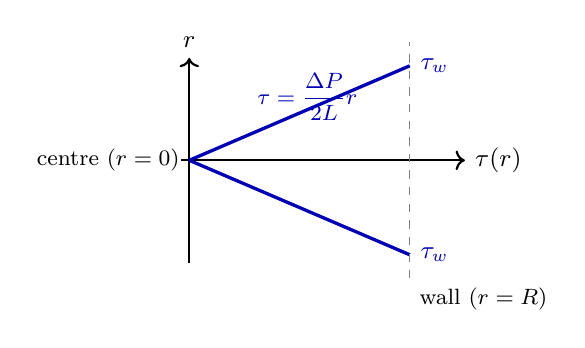
\begin{tikzpicture}[scale=1.0, every node/.style={font=\small}]
  % Shear stress profile (linear)
  \draw[->,thick] (0,-1.3) -- (0,1.3) node[above]{$r$};
  \draw[->,thick] (-0.1,0) -- (3.5,0) node[right]{$\tau(r)$};
  \draw[blue!70!black, very thick] (0,0) -- (2.8,1.2)
        node[right]{$\tau_w$};
  \draw[blue!70!black, very thick] (0,0) -- (2.8,-1.2)
        node[right]{$\tau_w$};
  \draw[dashed,gray] (2.8,-1.5) -- (2.8,1.5);
  \node[below right] at (2.8,-1.5) {\footnotesize wall ($r=R$)};
  \node[left] at (0,0) {\footnotesize centre ($r=0$)};
  % Arrow indicating linear
  \node[blue!70!black] at (1.5,0.8) {\footnotesize $\tau=\dfrac{\Delta P}{2L}r$};
\end{tikzpicture}
\caption{Shear stress profile inside the needle. The stress is always
linear in $r$, peaking at the wall with value $\tau_w=\Delta P\,R/2L$
and zero at the centreline. This universal result holds for any
constitutive model.}
\label{fig:stress_profile}
\end{figure}

\subsection{Cross-model extension (Rabinowitsch--Weissenberg)}
\label{sec:cross_HP}

\emph{Motivation.} The Cross model gives a physically correct rest viscosity
$\eta_0$ that the Power Law cannot represent. At very slow piston velocities
-- the safe operating end of the window for cell-loaded inks -- the Cross
model can predict pressures and wall shear rates that differ by an order of
magnitude from the Power-Law estimate. Accepting the extra numerical effort
of the Rabinowitsch--Weissenberg integral is therefore not optional for
production-quality predictions.

The Cross model has no closed-form $Q(\tau_w)$ expression. We use the
Rabinowitsch--Weissenberg integral:
\begin{equation}
Q(\tau_w) \;=\; \frac{\pi R^3}{\tau_w^3}
\int_0^{\tau_w} \tau^2\,\gd(\tau)\, d\tau,
\label{eq:rabinowitsch}
\end{equation}
where $\gd(\tau)$ is obtained by inverting Eq.~\ref{eq:cross} (solve
$\eta(\gd)\gd=\tau$ for $\gd$ numerically -- a single \texttt{fzero}
call per point). The MATLAB code at
\texttt{bioprinting\_algorithm\_v4.m} runs this on a 400-point grid
for each $V_p$.

\textbf{Why this integral is exact (for any constitutive model).}
The key insight is that the universal linear stress profile
$\tau(r)=(\Delta P/2L)r$ allows a change of integration variable from
$r$ to $\tau$. Writing $r=2L\tau/\Delta P$ and $dr=2L/\Delta P\,d\tau$,
and noting that $Q=2\pi\int_0^R v(r)r\,dr$ can be integrated by parts
(with $v(R)=0$):
\[
Q \;=\; \pi\int_0^R r^2\,\gd(r)\,dr
  \;=\; \frac{\pi R^3}{\tau_w^3}
        \int_0^{\tau_w}\!\tau^2\,\gd(\tau)\,d\tau.
\]
No assumption about the form of $\gd(\tau)$ has been made; the identity
holds for \emph{any} generalised Newtonian fluid.

\textbf{The Weissenberg--Rabinowitsch wall-shear-rate correction.}
Differentiating Eq.~\eqref{eq:rabinowitsch} with respect to $\tau_w$
yields the true wall shear rate from the apparent Newtonian value
$\gd_a\equiv 4Q/\pi R^3$:
\begin{equation}
\gd_w \;=\; \frac{1}{\pi R^3}
            \left(3Q + \tau_w\frac{dQ}{d\tau_w}\right)
     \;=\; \frac{3n'+1}{4n'}\cdot\frac{4Q}{\pi R^3},
\label{eq:WR_correction}
\end{equation}
where
\begin{equation}
n' \;\equiv\; \frac{d\ln\tau_w}{d\ln\gd_w}
\label{eq:nprime}
\end{equation}
is the \textbf{local log-log slope} of the flow curve $\tau_w$ vs
$\gd_w$ evaluated at the operating point. Three observations follow
immediately:
\begin{enumerate}[leftmargin=1.6em,itemsep=2pt]
\item \textbf{For the Power-Law model,} $n'=n$ everywhere (constant
  slope in log-log), so
  Eq.~\eqref{eq:WR_correction} reduces to the exact result from the
  derivation above: $\gd_w=\frac{3n+1}{4n}\cdot\frac{4Q}{\pi R^3}$.
\item \textbf{For the Cross model,} $n'$ varies with $\gd_w$
  (from $n'\to 1$ at very low $\gd_w$ in the Newtonian plateau to
  $n'\to 1-m$ in the power-law region, where $\eta\sim\gd^{-m}$ so
  $\tau\sim\gd^{\,1-m}$; for the NE, $m=0.988$ gives $n'\approx0.01$).
  The correction factor $(3n'+1)/(4n')$ must therefore be re-evaluated
  at each operating point; this is equivalent to evaluating the integral
  in Eq.~\eqref{eq:rabinowitsch} numerically.
\item \textbf{Connection to the generalised Reynolds number.}
  The same local slope $n'$ enters the Metzner--Reed
  $\Rey_\mathrm{gen}$ (Eq.~\ref{eq:re_gen}): both the laminar-flow
  validation and the wall-shear-rate correction share the same
  local-slope characterisation of the flow curve.
  Note that this $n'$ (slope of $\tau_w$ vs.\ the true wall shear rate
  $\gd_w$) and the Metzner--Reed $n'$ used in $\Rey_\mathrm{gen}$ (slope
  vs.\ the nominal rate $8\bar{v}/D$, Hydraulic-Loop chapter) are the
  same local log-log slope of the flow curve; for a power-law fluid
  they coincide exactly and the two uses are interchangeable.
\end{enumerate}

\subsection{Which model to trust?}

\emph{Motivation.} Using the Power-Law model outside its fitted shear-rate
range is a leading source of over-predicted pressures and spurious safety
failures. Knowing \emph{when} the Cross model differs materially from the
Power Law -- and why -- prevents the common mistake of dismissing an ink as
``unprintable'' because the Power-Law $\Delta P$ estimate exceeds the syringe
ceiling at a $V_p$ where the true Cross-model value is perfectly safe.

Both models are available in the MATLAB output, and they are compared
side-by-side.

\begin{itemize}[leftmargin=1.6em,itemsep=2pt]
\item \textbf{In the printable range} ($\gd_w\sim 50$--$1000\,\si{\per\s}$
  for 21G), both agree within 20\% for our inks.
\item \textbf{At low $\gd_w$} (very slow prints or 22G at low $V_p$):
  the Power Law over-estimates $\Delta P$ because it has no $\eta_0$
  plateau. The Cross model is correct.
\item \textbf{Preferred:} Cross for all production runs. Power Law
  reserved for quick back-of-envelope estimates.
\end{itemize}

\subsection{Wall shear rate and stress}
\label{sec:wall_shear}

\emph{Motivation.} $\Delta P$ and $\tau_w$ are both required, and they are
not interchangeable: $\Delta P$ is the mechanical load on the hardware;
$\tau_w$ is the biological stress on the cells. A print can be mechanically
safe ($\Delta P\ll$ syringe ceiling) yet biologically damaging
($\tau_w>\SI{5}{\kPa}$) -- or vice versa. Reporting either without the other
gives an incomplete safety picture.

Once $\tau_w$ is known, wall shear rate follows by inverting the
constitutive model:
\begin{equation}
\gd_w = (\tau_w/K)^{1/n} \;\text{(PL)}; \qquad
\gd_w\text{ by \texttt{fzero} on}\; \eta(\gd)\gd=\tau_w \;\text{(Cross)}.
\label{eq:gdot_w}
\end{equation}
$\gd_w$ is the shear rate cells see at the needle wall, and is the
disruption shear rate to use when evaluating the recovery test result.

\paragraph{Cell-safety threshold.}
Literature consensus places the upper bound for human cells at
$\tau_w\sim 5\,\si{\kPa}$ \citep{BlaeserEtAl2016}. Above this, cell
viability drops sharply. Both $\tau_w$ and cumulative shear exposure
(Ch.~\ref{sec:bio}) must be checked for cell-loaded prints.

\begin{examplebox}
Hagen--Poiseuille on 21G at $V_p=0.01\,\mms$ (Cross model):

\medskip\centering
\begin{tabular}{lcccc}
\toprule
Ink & $Q$ [\si{\mm^3/\s}] & $\tau_w$ [\si{\Pa}] & $\gd_w$ [\si{\per\s}] & $\Delta P$ [\si{\kPa}] \\
\midrule
C15           & 1.61 & 564  & 220 & 139 \\
C15 Gira 5.5  & 1.61 & 663  & 60  & 164 \\
Bozano        & 1.61 & 469  & 8   & 116 \\
\bottomrule
\end{tabular}

\medskip\flushleft
All three inks deliver the same $Q$ (geometry-fixed), but at very
different $\tau_w$ and $\gd_w$ -- the rheology decides. Pressures sit
at 100--170\,\si{\kPa}, well below the 1500\,\si{\kPa} syringe ceiling
and the 5\,\si{\kPa} cell-safe wall-shear ceiling.
\end{examplebox}

\begin{runningbox}{RUNNING EXAMPLE -- Solution to Q3}
\textbf{Question.} At $V_p=0.01\,\mms$ on 21G, is the extrusion
pressure safe for C15 Gira 5.5?

\medskip\textbf{From the worked example above:}
\[
\Delta P_\mathrm{Cross}\approx 164\,\si{\kPa}, \quad
\tau_w\approx 663\,\si{\Pa}, \quad
\gd_w\approx 60\,\si{\per\s}.
\]
\textbf{Safety check:}
\begin{itemize}[leftmargin=1.4em,itemsep=1pt]
\item Syringe ceiling 1500\,\si{\kPa}: $164/1500=11\%$. Comfortable.
\item Cell-safety $\tau_w<5\,\si{\kPa}$: 663\,\si{\Pa} is far below.
\item Motor stall (estimated $\sim 500$--$800\,\si{\kPa}$): comfortable.
\end{itemize}
\textbf{Verdict.} Safe to print. At $V_p=0.03\,\mms$, $\Delta P$
rises to $\sim 400\,\si{\kPa}$ (scaling as $V_p^{0.24}$ for
$n=0.24$) -- still safe but with smaller margin.

\medskip\emph{Still unknown:} the slicer Extrusion Multiplier. Q4.
\end{runningbox}

\begin{inpracticebox}
\textbf{Reading the MATLAB output: always check the trio $\Delta P$,
$\tau_w$, $\gd_w$.}

After running \texttt{run\_solver\_v4.m}, the output file and summary
plot report all three quantities for every $(V_p,\,\text{needle})$
combination. A safe operating point requires passing \emph{two
independent} checks:
\begin{enumerate}[leftmargin=1.6em,itemsep=2pt]
\item \textbf{Mechanical:} $\Delta P < \SI{1500}{\kPa}$ (BD 10~mL syringe
  rating). Most DIW inks clear this easily at bench-realistic $V_p$.
\item \textbf{Biological:} $\tau_w < \SI{5}{\kPa}$ (cell-safety ceiling,
  Eq.~\ref{sec:wall_shear}). This is the binding constraint for
  cell-loaded inks; note that $\tau_w=\Delta P\,R/2L$ grows with
  decreasing $R$, so a narrow needle can be mechanically fine yet
  biologically dangerous.
\end{enumerate}
Do not stop at $\Delta P$. A syringe pressure of \SI{300}{\kPa} is
perfectly safe for hardware, but for a 22G needle at that pressure
$\tau_w=\Delta P\,R/(2L)=300\times10^3\times0.2065\times10^{-3}/
(2\times25.4\times10^{-3})=\SI{1.22}{\kPa}$ -- safely below
\SI{5}{\kPa} in this case, but always verify explicitly; do not rely
on intuition. If $\tau_w$ exceeds the ceiling, the corrective action
is to increase $R$ (use a wider needle) or decrease $V_p$, not merely
to check the syringe rating.
\end{inpracticebox}

\begin{goingdeeperbox}
\textbf{Detecting wall slip (Mooney analysis).} Real DIW inks can slip at
the needle wall, inflating apparent flow. Mooney's test: measure the
apparent wall shear rate $\gd_{a}=4Q/\pi R^3$ at fixed wall stress
$\tau_w$ for needles of \emph{different} radii $R$ and plot $\gd_a$ vs.
$1/R$. A non-zero slope $=4 v_s(\tau_w)$ reveals a slip velocity $v_s$;
zero slope means no slip. Slip masquerades as shear thinning, so unflagged
slip corrupts $K,n$. This is the physical basis of the $f_\mathrm{slip}$
factor in $k_\mathrm{flow}$ (Eq.~\ref{eq:kflow}) \citep{Mooney1931}.
\end{goingdeeperbox}

% ---- Exercises --------------------------------------------------------
\subsection*{Check Yourself}
\label{sec:hp_exercises}

\begin{exercise}{\diffA}
A 21G needle has inner radius $R=\SI{0.2575}{\mm}$ and length
$L=\SI{31.75}{\mm}$. The Cross-model MATLAB solver predicts a wall shear
stress of $\tau_w=\SI{500}{\Pa}$ at a given $V_p$.
\begin{enumerate}[label=(\alph*),leftmargin=1.6em,itemsep=1pt]
  \item Use Eq.~\ref{eq:HP_PL} to compute the pressure drop $\Delta P$
    in \si{\kPa}.
  \item Is this $\Delta P$ within the syringe ceiling of \SI{1500}{\kPa}?
  \item Is $\tau_w$ within the cell-safety ceiling of \SI{5}{\kPa}?
\end{enumerate}
\begin{solution}
(a) $\Delta P = 2L\tau_w/R = 2\times\SI{31.75}{\mm}\times\SI{500}{\Pa}
    /\SI{0.2575}{\mm}$.
Convert all lengths to metres:
$L=\SI{0.03175}{\m}$, $R=\SI{2.575e-4}{\m}$.
\[
\Delta P = \frac{2\times0.03175\times500}{2.575\times10^{-4}}
         = \frac{31.75}{2.575\times10^{-4}}
         = \SI{1.233e5}{\Pa}
         \approx \SI{123.3}{\kPa}.
\]

(b) $\SI{123.3}{\kPa} < \SI{1500}{\kPa}$: within the syringe ceiling (8.2\% of rating). Comfortable.

(c) $\SI{500}{\Pa} = \SI{0.5}{\kPa} < \SI{5}{\kPa}$: within the cell-safety ceiling by a factor of 10.
\end{solution}
\end{exercise}

\begin{exercise}{\diffB}
A bioink follows the Power-Law model with $K=\SI{120}{\Pa\s^n}$ and
$n=0.25$. It is printed through a 21G needle ($R=\SI{0.2575}{\mm}$,
$L=\SI{31.75}{\mm}$) at a piston velocity $V_p=\SI{0.01}{\mm/\s}$
($Q\approx\SI{1.61}{\mm^3/\s}$; use this value directly).
\begin{enumerate}[label=(\alph*),leftmargin=1.6em,itemsep=1pt]
  \item Apply Eq.~\ref{eq:tau_w_PL} to compute $\tau_w$ in \si{\Pa}.
  \item Compute $\Delta P$ in \si{\kPa} via Eq.~\ref{eq:HP_PL}.
  \item Compute the true wall shear rate $\gd_w$ in \si{\per\s} by
    inverting the Power-Law (Eq.~\ref{eq:gdot_w}).
\end{enumerate}
\textit{(Use the stated round values; do not substitute the project-ink
parameters from the appendices.)}
\begin{solution}
\textbf{Step (a) -- Wall shear stress.}

First evaluate the argument of the Power-Law:
\[
\frac{(3n+1)Q}{\pi n R^3}
= \frac{(3\times0.25+1)\times1.61}{\pi\times0.25\times(0.2575)^3}.
\]
Numerator: $(0.75+1)\times1.61 = 1.75\times1.61 = \SI{2.8175}{\mm^3/\s}$.

Denominator: $\pi\times0.25\times(0.2575)^3$.
$(0.2575)^3 = 0.2575\times0.2575\times0.2575$.
$0.2575^2 = 0.066306$; $0.066306\times0.2575 = 0.017074\,\si{\mm^3}$.
$\pi\times0.25\times0.017074 = 0.78540\times0.017074 = \SI{0.013413}{\mm^3/\s}$
(the $Q$ units cancel, leaving \si{\per\s} after division).

\[
\frac{(3n+1)Q}{\pi n R^3}
= \frac{2.8175}{0.013413} = \SI{210.1}{\per\s}.
\]

Now raise to the power $n=0.25$:
$(210.1)^{0.25} = \sqrt{\sqrt{210.1}}$.
$\sqrt{210.1}\approx14.50$; $\sqrt{14.50}\approx3.808$.

\[
\tau_w = K\times(210.1)^{0.25} = 120\times3.808 = \SI{456.9}{\Pa}
       \approx \SI{457}{\Pa}.
\]

\textbf{Step (b) -- Pressure drop.}

\[
\Delta P = \frac{2L\tau_w}{R}
         = \frac{2\times31.75\,\si{\mm}\times457\,\si{\Pa}}{0.2575\,\si{\mm}}
         = \frac{29{,}017}{0.2575}\,\si{\Pa}
         = \SI{112{,}689}{\Pa}
         \approx \SI{112.7}{\kPa}.
\]

\textbf{Step (c) -- Wall shear rate (PL inversion).}

\[
\gd_w = \left(\frac{\tau_w}{K}\right)^{1/n}
      = \left(\frac{457}{120}\right)^{1/0.25}
      = (3.808)^{4}.
\]
$(3.808)^2 = 14.50$; $(3.808)^4 = (14.50)^2 = 210.3\,\si{\per\s}$.

As expected, $\gd_w\approx\SI{210}{\per\s}$ -- this is consistent with
the argument evaluated in (a), confirming the algebra is self-consistent.
\end{solution}
\end{exercise}

\begin{exercise}{\diffC}
A researcher suspects wall slip in a CMC hydrogel and performs a Mooney
test at fixed wall stress $\tau_w=\SI{400}{\Pa}$. Measuring the apparent
wall shear rate $\gd_a = 4Q/\pi R^3$ at two needle radii gives:
\begin{center}
\begin{tabular}{lcc}
\toprule
Needle & $R$ [\si{\mm}] & $\gd_a$ [\si{\per\s}] \\
\midrule
21G & 0.2575 & 180 \\
22G & 0.2065 & 260 \\
\bottomrule
\end{tabular}
\end{center}
\begin{enumerate}[label=(\alph*),leftmargin=1.6em,itemsep=1pt]
  \item Plot $\gd_a$ vs.\ $1/R$ (identify the two data points and their
    coordinates) and compute the slope.
  \item Extract the slip velocity $v_s$ from the slope and comment on
    its magnitude relative to typical mean needle velocities.
  \item If wall slip is confirmed, does the fitted Power-Law index $n$
    overestimate or underestimate shear thinning? Explain.
\end{enumerate}
\begin{solution}
\textbf{Step (a) -- Mooney plot coordinates.}

$1/R_1 = 1/0.2575 = \SI{3.883}{\per\mm}$, $\gd_{a1}=\SI{180}{\per\s}$.

$1/R_2 = 1/0.2065 = \SI{4.842}{\per\mm}$, $\gd_{a2}=\SI{260}{\per\s}$.

Slope:
\[
m_\mathrm{Mooney}
= \frac{\gd_{a2}-\gd_{a1}}{1/R_2-1/R_1}
= \frac{260-180}{4.842-3.883}
= \frac{80}{0.959}
= \SI{83.4}{\per\s\cdot\mm}
= \SI{83.4}{\mm/\s}\cdot\si{\mm^{-1}}\cdot\si{\mm}
= \SI{83.4}{\mm/\s}.
\]
(Units: $[\gd_a] = \si{\per\s}$, $[1/R]=\si{\per\mm}$, so slope
has dimensions of \si{\mm/\s}.)

\textbf{Step (b) -- Slip velocity.}

The Mooney relation is $\gd_a(\tau_w) = \gd_\mathrm{true}(\tau_w) +
4v_s(\tau_w)/R$, so a plot of $\gd_a$ vs.\ $1/R$ at fixed $\tau_w$
has slope $=4v_s$:
\[
v_s = \frac{m_\mathrm{Mooney}}{4} = \frac{83.4}{4}
    = \SI{20.8}{\mm/\s}.
\]
At $V_p=\SI{0.01}{\mm/\s}$ the mean needle velocity for 21G is
$\bar v_n = 771\times0.01=\SI{7.71}{\mm/\s}$. A slip velocity of
\SI{20.8}{\mm/\s} is nearly three times this mean velocity -- a very
large fraction of the measured flow rate is wall slip, not true bulk
shear. The apparent flow curve is severely contaminated.

\textbf{Step (c) -- Effect on fitted $n$.}

Wall slip adds an $R$-dependent excess to the apparent $\gd_a$ that
scales as $\sim 1/R$ rather than the $\sim 1/R^3$ dependence of the
true wall shear rate. At small $R$ (narrow needles, high $1/R$), the
slip contribution proportionally inflates $\gd_a$ more, making
$\tau_w(\gd_a)$ appear to flatten more quickly with $\gd_a$ than it
would in a true bulk measurement. Fitting $\tau=K\gd^n$ to the
slip-contaminated data therefore yields a \emph{lower} apparent $n$
(more shear-thinning) than the true bulk behaviour -- i.e., $n$ is
\emph{underestimated}. Equivalently, $K$ is overestimated. Both errors
inflate the predicted $\Delta P$ at high $\gd_w$.
\end{solution}
\end{exercise}

\begin{takeawaybox}
\begin{itemize}[leftmargin=1.4em,itemsep=2pt]
\item The shear stress profile $\tau(r)=(\Delta P/2L)r$ is universal and
  linear -- wall stress is always the maximum.
\item $\Delta P\propto R^{-4}$: needle gauge is the dominant lever.
  Cross-model prediction is preferred over Power Law for all
  multi-decade ranges.
\item $\tau_w<5\,\si{\kPa}$ is the cell-safety constraint. All three
  inks satisfy it comfortably at the nominal $V_p$.
\end{itemize}
\end{takeawaybox}

\begin{designrulebox}
\textbf{DR 4.1.} Always report $\Delta P$, $\tau_w$, and $\gd_w$ as a
trio when characterising a print condition. $\Delta P$ alone is
insufficient -- $\tau_w$ determines cell survival.

\textbf{DR 4.2.} Use the Cross model for $\Delta P$ prediction. Report
both Cross and Power Law outputs so inconsistencies can be flagged.

\textbf{DR 4.3.} For any new ink or needle combination, always run
$\Rey_\mathrm{gen}$ and $\Bi$ estimates \emph{before} the first print
to confirm laminar flow and to anticipate the velocity profile type.
\end{designrulebox}

% =================================================================
\section{Temperature and Process-Robustness}
\label{sec:temperature}

\emph{Motivation.} Everything so far assumed a fixed temperature and an ideal wall. Two
real-world levers move the rheology under your feet: \emph{temperature}
and \emph{flow instabilities}. This short chapter gives the theory you
need to keep a print reproducible across a warm afternoon and a cold lab.

\subsection{Temperature dependence of viscosity}
\begin{intuitionbox}
Viscosity falls as temperature rises: molecules jump their neighbours'
cages more easily. A few degrees of drift can change $\Delta P$ and bead
width enough to fail a print --- so either control $T$ or measure its
slope.
\end{intuitionbox}

For most aqueous gels well above any glass transition, the
\textbf{Arrhenius} form holds:
\begin{equation}
\eta(T)=\eta_\infty\,\exp\!\left(\frac{E_a}{RT}\right),
\label{eq:arrhenius}
\end{equation}
where $E_a$ (\si{\J/\mol}) is the flow activation energy and
$R=8.314$\,\si{\J/\mol/\K}. A plot of $\ln\eta$ vs.\ $1/T$ is linear
with slope $E_a/R$.

\begin{derivationbox}[title={DERIVATION --- Arrhenius: two-point method and small-$\Delta T$ sensitivity}]

\textbf{Two-point method.}
Write Eq.~\ref{eq:arrhenius} at two temperatures $T_1$ and $T_2$:
\[
  \ln\eta_1 = \ln\eta_\infty + \frac{E_a}{RT_1}, \qquad
  \ln\eta_2 = \ln\eta_\infty + \frac{E_a}{RT_2}.
\]
Subtract to eliminate $\eta_\infty$:
\[
  \ln\frac{\eta_1}{\eta_2}
    = \frac{E_a}{R}\!\left(\frac{1}{T_1}-\frac{1}{T_2}\right).
\]
Solving for $E_a$:
\begin{equation}
E_a
  = \frac{R\,\ln(\eta_1/\eta_2)}{1/T_1 - 1/T_2}.
\label{eq:ea_twopoint}
\end{equation}
This requires only two viscosity measurements at two temperatures;
no pre-knowledge of $\eta_\infty$ is needed.

\medskip\noindent\textbf{Small-drift sensitivity.}
Differentiate Eq.~\ref{eq:arrhenius} with respect to $T$:
\[
  \frac{d\eta}{dT} = -\frac{E_a}{RT^2}\,\eta(T).
\]
Divide both sides by $\eta(T)$:
\[
  \frac{d\ln\eta}{dT} = -\frac{E_a}{RT^2}.
\]
For a small temperature excursion $\Delta T$ (a few degrees), the
fractional viscosity change is therefore:
\begin{equation}
\frac{\Delta\eta}{\eta}
  \;\approx\; e^{-(E_a/RT^2)\,\Delta T} - 1
  \;\approx\; -\frac{E_a}{RT^2}\,\Delta T
  \quad\text{(first-order)}.
\label{eq:arrhenius_sensitivity}
\end{equation}
The same proportional change in $\eta$ propagates into $\Delta P$ via
Hagen--Poiseuille, so a $\pm1\,\si{\celsius}$ drift at
$T=293\,\si{\K}$ causes a fractional $\Delta P$ shift of
$\approx\pm(E_a/RT^2)$, independent of needle gauge or $V_p$.
\end{derivationbox}

\begin{goingdeeperbox}
\textbf{When Arrhenius fails: WLF.} Near a glass/gel transition
($T<T_g+100$\,K) the temperature dependence is super-Arrhenius and the
Williams--Landel--Ferry equation applies to the shift factor $a_T$:
\begin{equation}
\log_{10} a_T=\frac{-C_1\,(T-T_\mathrm{ref})}{C_2+(T-T_\mathrm{ref})},
\label{eq:wlf}
\end{equation}
with ``universal'' $C_1\approx17.4$, $C_2\approx51.6$\,K when
$T_\mathrm{ref}=T_g$. For the dilute aqueous CMC/NE inks here, Arrhenius
(Eq.~\ref{eq:arrhenius}) is the practical choice; WLF matters for
concentrated or near-gelation formulations \citep{WLF1955}.
\end{goingdeeperbox}

\begin{inpracticebox}
Measure $\eta$ at $T_\mathrm{lab}\pm5\,\si{\celsius}$, fit $E_a$ via
Eq.~\ref{eq:ea_twopoint}, and report the \%-change in $\Delta P$ per
\si{\celsius} using Eq.~\ref{eq:arrhenius_sensitivity}. If it exceeds
your pressure margin, thermostat the syringe.
\end{inpracticebox}

\subsection{Flow instabilities and the smooth-filament limit}
Even laminar, isothermal extrusion has an upper usable rate. Above a
critical wall stress the extrudate stops being smooth: \emph{sharkskin}
(surface mattness), then \emph{gross melt fracture} (helical/chaotic
distortion). The onset is an \emph{elastic} instability, governed by the
Weissenberg number $\mathrm{Wi}=N_1/(2\tau_w)=S_R$
(Eq.~\ref{eq:recoverable}) and the Deborah number rather than by Reynolds
number.

\begin{inpracticebox}
The ``rough filament / extrudate distortion'' failure mode
(Ch.~\ref{sec:failures}) is this instability. Corrective action: lower
$V_p$ (reduce $\tau_w$ and $S_R$), widen the needle, or raise $T$ to drop
viscosity --- all reduce the stored elastic strain at exit.
\end{inpracticebox}

\subsection{Reproducibility checklist}
\begin{enumerate}[leftmargin=1.6em,itemsep=2pt]
\item Record lab $T$ at print time; keep the syringe within
  $\pm2\,\si{\celsius}$.
\item Re-fit $K,n$ if $T$ drifts more than your measured $E_a$ tolerance
  allows (Eq.~\ref{eq:arrhenius_sensitivity}).
\item Stay below the onset of surface distortion (keep $S_R$ modest;
  see Eq.~\ref{eq:tanner}).
\item Re-run recovery if the batch or storage time changed (thixotropy
  ages: \citealp{Barnes1997,Mewis2009}).
\end{enumerate}

\subsection*{Check Yourself}

\begin{exercise}{\diffA}
An ink has $E_a=\SI{30}{\kJ/\mol}$ at a lab temperature of
$T=\SI{293}{\K}$. Estimate the fractional viscosity change for a
$+5\,\si{\celsius}$ rise using the small-drift approximation
(Eq.~\ref{eq:arrhenius_sensitivity}).

\begin{solution}
$E_a/R = 30000/8.314 = 3608\,\si{\K}$.

$\Delta\ln\eta \approx -(E_a/RT^2)\,\Delta T
= -3608\times5/293^2
= -18040/85849
= -0.210.$

Fractional change $= e^{-0.210}-1 = 0.810 - 1 = -0.190$, i.e., viscosity
drops $\approx19\%$ per $5\,\si{\celsius}$ rise.

Note: the first-order approximation $\approx-E_a\Delta T/(RT^2)=-0.210$
agrees well because $|\Delta\ln\eta|\ll1$.
\end{solution}
\end{exercise}

\begin{exercise}{\diffB}
Two-point Arrhenius. An ink has $\eta=\SI{100}{\Pa\s}$ at
$T_1=\SI{293}{\K}$ and $\eta=\SI{70}{\Pa\s}$ at $T_2=\SI{303}{\K}$.
Use Eq.~\ref{eq:ea_twopoint} to find $E_a$.

\begin{solution}
$\ln(100/70) = \ln(10/7) = 0.3567$.

$1/T_1 - 1/T_2 = 1/293 - 1/303 = (303-293)/(293\times303)
= 10/88779 = 1.126\times10^{-4}\,\si{\per\K}$.

$E_a = R\,\ln(\eta_1/\eta_2)\,/\,(1/T_1-1/T_2)
= 8.314\times0.3567/1.126\times10^{-4}
= 2.965/1.126\times10^{-4}
= 2.63\times10^4\,\si{\J/\mol}
\approx \SI{26.3}{\kJ/\mol}$.

(Some rounding conventions give $26.4$\,kJ/mol; the spread reflects
significant-figure choices in $\ln(10/7)$ and the denominator.)
\end{solution}
\end{exercise}

\begin{exercise}{\diffC}
Explain why extrudate distortion (melt fracture) at the needle exit
scales with the Weissenberg number rather than the Reynolds number for
CMC/NE inks.

\begin{solution}
The generalised Reynolds number $\Rey_\mathrm{gen}\ll1$ for these
high-viscosity inks (typically $\mathcal{O}(10^{-3})$--$\mathcal{O}(10^{-1})$),
so inertial forces are negligible and the flow is deeply laminar.
Extrudate distortion is therefore not an inertial (Kelvin--Helmholtz-type)
instability but an \emph{elastic} one: at high $V_p$ the polymer chains
are highly stretched inside the needle, storing elastic energy
characterised by the first normal stress difference $N_1$. At the exit
the confinement is removed and the stored elastic strain
$S_R = N_1/(2\tau_w)$ (Eq.~\ref{eq:recoverable}) is released
non-uniformly across the cross-section, destabilising the free surface.
The Weissenberg number $\mathrm{Wi} = S_R$ is the dimensionless ratio of
elastic to viscous stresses; once $S_R$ exceeds an $\mathcal{O}(1)$
threshold the surface buckles into sharkskin or chaotic fracture.
Corrective actions that lower $S_R$ --- reducing $V_p$, switching to a
wider needle, or raising $T$ to decrease viscosity and relax the chains
faster --- all delay or prevent the onset.
\end{solution}
\end{exercise}

\begin{takeawaybox}
\begin{itemize}[leftmargin=1.4em,itemsep=2pt]
\item Viscosity is exponentially sensitive to temperature (Arrhenius);
  even $\pm2\,\si{\celsius}$ drift can shift $\Delta P$ and bead width
  measurably if $E_a$ is large.
\item The two-point method (Eq.~\ref{eq:ea_twopoint}) gives $E_a$ from
  just two flow-curve runs at different temperatures; report it for every
  ink used outside $20\pm2\,\si{\celsius}$.
\item Extrudate distortion is an elastic instability (Wi, not Re): lower
  $V_p$ or raise $T$ to reduce the recoverable strain $S_R$ at the exit.
\item Thixotropy ages with batch and storage: re-run recovery if the ink
  is more than a day old.
\end{itemize}
\end{takeawaybox}

\begin{designrulebox}
\textbf{DR T.1.} For any ink used outside the characterisation temperature
$T_0\pm2\,\si{\celsius}$, measure $\eta$ at two temperatures, compute
$E_a$ (Eq.~\ref{eq:ea_twopoint}), and report the fractional $\Delta P$
sensitivity per \si{\celsius} to the print log.

\textbf{DR T.2.} Keep the recoverable strain $S_R$ (Eq.~\ref{eq:recoverable})
below the surface-distortion onset. If rough filaments appear, reduce
$V_p$ by 20\% increments or switch to the next wider needle before
adjusting any slicer compensation.
\end{designrulebox}

% =================================================================
\section{Flow Factor, Die Swell, and the Slicer Translation}
\label{sec:flow_factor}

\emph{Why this chapter matters.}
A conventional FFF slicer assumes that the Extrusion Multiplier is
close to~1.0 and that deposited filament width equals the nozzle
diameter. Neither assumption holds for DIW: three independent physical
mechanisms shift the deposited volume away from the commanded volume,
and ignoring them produces systematically wrong line widths and
layer heights that accumulate across every layer of a multi-layer
scaffold. This chapter derives each mechanism, assembles them into
$k_\mathrm{flow}$ (Eq.~\ref{eq:kflow}), and shows how to translate
that diagnostic into the single number the slicer needs.

The slicer treats the printer as FFF. It multiplies the commanded
volumetric flow by an Extrusion Multiplier $\mathrm{EM}_\mathrm{slicer}$,
which in FFF normally sits near 1.0. In DIW, three independent physical
deviations change the effective deposited volume:

\begin{enumerate}[leftmargin=1.6em,itemsep=2pt]
\item \textbf{Die swell} ($\beta_\mathrm{swell}$): after leaving the
needle, viscoelastic ink expands radially as stored elastic stresses
relax. The deposited filament is wider than the needle ID.
$w_\mathrm{line}/\mathrm{ID}=1+\beta_\mathrm{swell}$.
\item \textbf{Syringe-wall slip} ($f_\mathrm{slip}\leq 1$): imperfect
piston sealing or ink-wall slip reduces the actual volume leaving the
needle. Default 1.0 until C2 calibration.
\item \textbf{Viscoelastic recovery penalty} ($\sqrt{R_\mathrm{rec}}$):
if the network has only partially recovered when the next layer arrives,
the deposited bead has not stiffened back up; material spreads and
effective cross-sectional volume is lost.
\end{enumerate}

\begin{equation}
k_\mathrm{flow}
\;=\; (1+\beta_\mathrm{swell})^{2}\,f_\mathrm{slip}\,\sqrt{R_\mathrm{rec}}.
\label{eq:kflow}
\end{equation}

\begin{figure}[h]
\centering
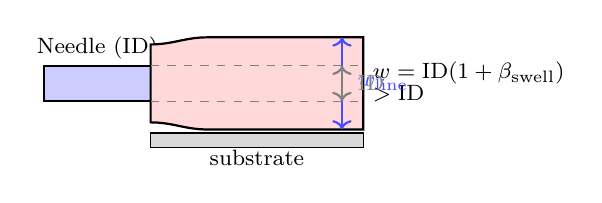
\begin{tikzpicture}[every node/.style={font=\small}, scale=0.9]
  % Needle exit
  \draw[thick, fill=blue!20] (0,0.25) rectangle (1.5,0.75);
  \node at (0.75,1.0) {\footnotesize Needle (ID)};
  % Filament with swell
  \draw[thick, fill=red!15] (1.5,-0.05) to[out=0,in=180] (2.3,-0.15)
    -- (4.5,-0.15) -- (4.5,1.15) -- (2.3,1.15)
    to[out=180,in=0] (1.5,1.05) -- cycle;
  \draw[dashed,gray] (1.5,0.25) -- (4.5,0.25);
  \draw[dashed,gray] (1.5,0.75) -- (4.5,0.75);
  % Labels
  \node[right] at (4.5,0.65) {\footnotesize $w=\mathrm{ID}(1+\beta_\mathrm{swell})$};
  \node[right] at (4.5,0.35) {\footnotesize $>\mathrm{ID}$};
  \draw[<->,thick,blue!70] (4.2,-0.15) -- (4.2,1.15)
    node[midway,right=2pt]{\footnotesize $w_\mathrm{line}$};
  \draw[<->,thick,gray] (4.2,0.25) -- (4.2,0.75)
    node[midway,right=2pt]{\footnotesize ID};
  % Substrate
  \draw[fill=gray!30] (1.5,-0.4) rectangle (4.5,-0.2);
  \node at (3,-0.55) {\footnotesize substrate};
\end{tikzpicture}
\caption{Die swell: the deposited filament is wider than the needle ID
because elastic stresses stored during confinement in the needle relax
on exit. Inks with $m\to 1$ (narrow transition) store little elastic
energy and swell minimally. Inks with $m<0.7$ may swell by
$\beta>0.15$ and require direct measurement in calibration test C1.}
\label{fig:dieswell}
\end{figure}

% ---- Derivation of every k_flow factor ----
\begin{derivationbox}[title={DERIVATION --- Each factor in $k_\mathrm{flow}=(1+\beta_\mathrm{swell})^2 f_\mathrm{slip}\sqrt{R_\mathrm{rec}}$}]
We derive each of the three dimensionless factors in Eq.~\ref{eq:kflow}
from first principles and then assemble the full expression.

\medskip\noindent\textbf{Factor 1 --- Die-swell area term
$(1+\beta_\mathrm{swell})^{2}$.}

\emph{Setup.} Define the swell ratio so that the deposited bead has
width
\begin{equation}
w \;=\; \mathrm{ID}\,(1+\beta_\mathrm{swell}),
\qquad \beta_\mathrm{swell}\geq 0.
\label{eq:swell_width}
\end{equation}
The slicer models a cylindrical filament of cross-sectional area
$A_\mathrm{ref}=\pi(\mathrm{ID}/2)^{2}$ per unit length of travel.

\emph{Actual cross-section.}
For a bead whose cross-section scales with the square of its lateral
width (the bead spreads uniformly in both transverse directions), the
deposited cross-sectional area is
\begin{equation}
A_\mathrm{dep}
\;=\; A_\mathrm{ref}\left(\frac{w}{\mathrm{ID}}\right)^{2}
\;=\; A_\mathrm{ref}(1+\beta_\mathrm{swell})^{2}.
\label{eq:Adep}
\end{equation}

\emph{Volume per unit length.}
Volume deposited per unit nozzle travel $= A_\mathrm{dep}\cdot\ell
= A_\mathrm{ref}(1+\beta_\mathrm{swell})^{2}\cdot\ell$,
while the slicer assumes $A_\mathrm{ref}\cdot\ell$. The ratio of
deposited to commanded volume per unit travel is therefore:
\begin{equation}
\frac{V_\mathrm{dep}}{V_\mathrm{cmd}}\Bigg|_\mathrm{swell}
\;=\; (1+\beta_\mathrm{swell})^{2}.
\label{eq:swell_factor}
\end{equation}
This factor exceeds 1 whenever $\beta_\mathrm{swell}>0$: swell deposits
\emph{more} material per unit length than commanded, so $k_\mathrm{flow}$
is driven above the slip and recovery baseline.

\medskip\noindent\textbf{Factor 2 --- Slip factor $f_\mathrm{slip}\leq 1$.}

\emph{Definition.}
In an ideal piston-driven system (no seal leak, no ink-barrel slip), a
piston displacement $\delta x$ sweeps a volume $A_\mathrm{piston}\,\delta x$
that exits entirely through the needle. In practice, imperfect sealing
or slip at the ink--barrel interface means only a fraction of that swept
volume actually exits:
\begin{equation}
V_\mathrm{exit}
\;=\; f_\mathrm{slip}\,A_\mathrm{piston}\,\delta x,
\qquad 0 < f_\mathrm{slip}\leq 1.
\label{eq:fslip_def}
\end{equation}
Equivalently,
\begin{equation}
f_\mathrm{slip}
\;=\;
\frac{V_\mathrm{exit}}{V_\mathrm{swept}}\,.
\label{eq:fslip_ratio}
\end{equation}
A value $f_\mathrm{slip}<1$ reduces the actual flow rate below the
slicer's assumed value, causing under-extrusion. Experimentally,
$f_\mathrm{slip}$ is determined from the C2 calibration (mass-per-line
test). For well-sealed syringes with low-viscosity inks, $f_\mathrm{slip}
\approx 1.0$; for high-viscosity bioinks with marginal sealing, values as
low as 0.8 have been reported.

\medskip\noindent\textbf{Factor 3 --- Viscoelastic recovery penalty
$\sqrt{R_\mathrm{rec}}$.}

\emph{Physical argument (semi-empirical).}
When a hydrogel bead is deposited, its microstructure has been
disrupted by the high shear inside the needle. If the inter-layer
dwell time is shorter than the network's relaxation time, the network
is only partially recovered (recovery fraction $R_\mathrm{rec}<1$) when
the next layer arrives.

A bead with $R_\mathrm{rec}<1$ has a lower effective elastic modulus
$G'_\mathrm{eff}\approx R_\mathrm{rec}\,G'_0$. The restorative elastic
stress that opposes lateral spreading of the bead scales with
$G'_\mathrm{eff}$. Under a gravitational or contact load, the equilibrium
lateral deformation (and hence the bead width $w$) scales as
$(G'_\mathrm{eff})^{-1/2}$~--- a softer bead deforms more in proportion to
the square root of its compliance. Because bead width $\propto
(R_\mathrm{rec})^{-1/2}$ and the locked-in area scales with $w^2$,
the ratio of \emph{effectively retained} bead volume to a fully
recovered ($R_\mathrm{rec}=1$) bead scales as
\begin{equation}
\frac{V_\mathrm{retained}}{V_\mathrm{ref}}\Bigg|_\mathrm{rec}
\;\propto\; \sqrt{R_\mathrm{rec}}\,.
\label{eq:Rrec_factor}
\end{equation}
\textbf{Note:} this is a physically motivated scaling argument, not
an exact theorem. The exponent $\tfrac{1}{2}$ captures the dominant
dependence observed across hydrogel systems; materials with strongly
non-affine network response may deviate. Direct C2 calibration is
preferred over purely analytic estimates when $R_\mathrm{rec}<50\%$.

\medskip\noindent\textbf{Assembly.}
Multiplying the three independent contributions, the overall deposition
efficiency is
\begin{equation}
k_\mathrm{flow}
\;=\;
\underbrace{(1+\beta_\mathrm{swell})^{2}}_{\text{swell area}}
\;\cdot\;
\underbrace{f_\mathrm{slip}}_{\text{seal/slip}}
\;\cdot\;
\underbrace{\sqrt{R_\mathrm{rec}}}_{\text{recovery}}.
\tag{\ref{eq:kflow} restated}
\end{equation}
The slicer Extrusion Multiplier is the inverse of this efficiency:
\begin{equation}
\mathrm{EM}_\mathrm{slicer}
\;=\;
\frac{1}{k_\mathrm{flow}}
\;=\;
\frac{1}{(1+\beta_\mathrm{swell})^{2}\,f_\mathrm{slip}\,\sqrt{R_\mathrm{rec}}}\,.
\tag{\ref{eq:EM_slicer} restated}
\end{equation}
This inversion is the step most often missed in practice: $k_\mathrm{flow}$
is a diagnostic; $\mathrm{EM}_\mathrm{slicer}=1/k_\mathrm{flow}$ is
the control input.
\end{derivationbox}

\subsection{The crucial inversion: $k_\mathrm{flow}$ is not the number you type into the slicer}
\label{sec:kflow_inversion}

\emph{Motivation.}
Every DIW slicer that has an ``Extrusion Multiplier'' field is asking
for the factor by which to \emph{scale up} the commanded volumetric
flow to achieve the target deposited volume. Because $k_\mathrm{flow}$
is the \emph{efficiency} (deposited/commanded), the multiplier must be
its reciprocal. Entering $k_\mathrm{flow}$ directly is the most
common single-number error in DIW printing, and it compounds: if
$k_\mathrm{flow}=0.67$ and the operator types $0.67$, the under-build
worsens by a further factor of $0.67$ on top of the original deficit.

$k_\mathrm{flow}$ (Eq.~\ref{eq:kflow}) is the \textbf{deposition
efficiency}: the fraction of the slicer-commanded volume that ends up
locked in the bead:
\begin{equation}
k_\mathrm{flow}
\;=\;
\frac{\text{volume locked in bead}}
     {\text{volume slicer was told to deliver}}.
\label{eq:kflow_meaning}
\end{equation}
The slicer's Extrusion Multiplier is the \emph{control knob} the
operator uses to compensate for this inefficiency:
\begin{equation}
\boxed{\;\mathrm{EM}_\mathrm{slicer}
\;=\;
\frac{1}{k_\mathrm{flow}}
\;=\;
\frac{1}{(1+\beta_\mathrm{swell})^{2}\,f_\mathrm{slip}\,\sqrt{R_\mathrm{rec}}}\,.\;}
\label{eq:EM_slicer}
\end{equation}

\begin{warningbox}
\textbf{The single most common operational error in DIW.}
Reading $k_\mathrm{flow}=0.67$ from the CSV and typing $0.67$ into
the slicer \emph{worsens} under-build by another factor of $1/0.67
\approx 1.5$. The slicer multiplier is \textbf{always the inverse}:
$\mathrm{EM}=1/k_\mathrm{flow}$. When in doubt, verify from first
principles: if the bead is too thin (under-extrusion), $\mathrm{EM}$
must go \emph{up}.
\end{warningbox}

\paragraph{Physical interpretation:}
\begin{itemize}[leftmargin=1.4em,itemsep=2pt]
\item $k_\mathrm{flow}<1$: bead loses material to swell-then-spread or
  recovery-limited slump. Slicer under-builds at nominal volume; raise
  $\mathrm{EM}$ above 1.
\item $k_\mathrm{flow}>1$: bead locks in more volume than nominal
  (high recovery + large swell combine). Slicer over-builds; lower
  $\mathrm{EM}$ below 1.
\item $k_\mathrm{flow}=1$: perfect FFF analogy; $\mathrm{EM}=1$.
\end{itemize}

\subsection{Die-swell proxy from Cross $m$}

\emph{Motivation.}
Die swell requires knowledge of $\beta_\mathrm{swell}$, which
is strictly a post-extrusion measurement. When no direct measurement
is available (e.g.\ during ink design or simulation before printing),
the Cross sharpness exponent $m$ provides a physically grounded
first estimate: a high $m$ (sharp, cooperative transition) corresponds
to low elastic energy storage during flow, and hence minimal swell.

Die swell is driven by stored elastic energy. An ink with $m\to 1$
(sharp transition) stores very little elastic energy during
shear-thinning -- hence minimal swell. Empirical proxy:
\begin{equation}
\beta_\mathrm{swell} \;\approx\; 0.30\,(1-m).
\label{eq:beta_proxy}
\end{equation}
This spans $\beta=0$ ($m=1$, no swell) to $\beta=0.30$ ($m=0$, 30\%
swell). Direct measurement in C1 is preferred when $m<0.7$.

\begin{goingdeeperbox}
\textbf{Where die swell comes from: the first normal-stress difference.}
In shear, a viscoelastic fluid develops a normal-stress difference
$N_1=\tau_{xx}-\tau_{yy}>0$ that stores elastic energy. The recoverable
shear strain is
\begin{equation}
S_R=\frac{N_1}{2\tau_w}.
\label{eq:recoverable}
\end{equation}
On exit, that stored strain relaxes and the extrudate swells. Tanner's
relation links the swell ratio $B=D_\mathrm{extrudate}/D_\mathrm{die}$ to
$S_R$:
\begin{equation}
B \;=\; 0.13+\Bigl[\,1+\tfrac{1}{2}S_R^{\,2}\,\Bigr]^{1/6},
\label{eq:tanner}
\end{equation}
where the $0.13$ is the inertia-less Newtonian baseline swell. So
$\beta_\mathrm{swell}=B-1$ is \emph{elastic} in origin. A high Cross $m$
(sharp, cooperative thinning --- NE $m=0.988$) stores little elastic
strain $\Rightarrow$ small $S_R$ $\Rightarrow$ minimal swell, which is why
the empirical Cross-$m$ proxy used above works \citep{Tanner1970}.
\end{goingdeeperbox}

\begin{examplebox}
Predicted deposition efficiency and slicer Extrusion Multiplier
($f_\mathrm{slip}=1$, $R_\mathrm{rec}$ at $\gd_w\sim 100\,\si{\per\s}$):

\medskip\centering
\begin{tabular}{lccccc}
\toprule
Ink & $m$ & $\beta_\mathrm{swell}$ & $R_\mathrm{rec}$ [\%]
  & $k_\mathrm{flow}$ & $\mathrm{EM}_\mathrm{slicer}=1/k_\mathrm{flow}$ \\
\midrule
C15           & 0.811 & 0.057 & 60 & 0.86 & \textbf{1.17} \\
C15 Gira 5.5  & 0.988 & 0.004 & 45 & 0.67 & \textbf{1.49} \\
Bozano        & 0.866 & 0.040 & 98 & 1.07 & \textbf{0.93} \\
\bottomrule
\end{tabular}

\medskip\flushleft
The NE is the most demanding ink because of its low recovery: it
requires $\sim 49\%$ more material at the slicer than the nominal
FFF command. Bozano, with near-full recovery, actually asks for a
$\sim 7\%$ reduction.
\end{examplebox}

\begin{runningbox}{RUNNING EXAMPLE -- Solution to Q4}
\textbf{Question.} What Extrusion Multiplier should Ana enter for
C15 Gira 5.5?

\medskip\textbf{Step 1 -- compute $k_\mathrm{flow}$.}
$\beta_\mathrm{swell}=0.30(1-0.988)=0.004$. $f_\mathrm{slip}=1.0$.
$R_\mathrm{rec}\approx 45\%$ at $\gd_w\approx 60\,\si{\per\s}$:
\[
k_\mathrm{flow} = (1.004)^2\cdot 1.0\cdot\sqrt{0.45} \approx 0.67.
\]
\textbf{Step 2 -- invert.} $\mathrm{EM}_\mathrm{slicer}=1/0.67\approx\mathbf{1.49}$.

\textbf{Why $\mathrm{EM}>1$?} The NE has the lowest recovery (45\%)
of the three inks. Material leaves the needle but does not stiffen
quickly enough before the next layer arrives; it spreads and loses
effective cross-sectional volume. Pushing 49\% more compensates.

\medskip\emph{Still unknown:} will a 20-mm block survive its own
weight? Q5.
\end{runningbox}

\begin{inpracticebox}
\textbf{Calibrating $k_\mathrm{flow}$ at the bench (C2 protocol).}
\begin{enumerate}[leftmargin=1.6em,itemsep=3pt]
\item \textbf{Measure $\beta_\mathrm{swell}$ directly (C1).} Extrude a
  single line at your target $V_p$ onto a hydrophobic surface. After
  $\sim\SI{30}{\s}$, image the free-standing bead from above and measure
  its width $w$ with a calibrated micrograph. Then
  $\beta_\mathrm{swell}=(w/\mathrm{ID})-1$. Repeat 3 times and average.
\item \textbf{Measure $R_\mathrm{rec}$.} Read the structural recovery
  percentage from the 3-interval thixotropy test (Rheocompass output at
  the shear rate nearest your computed $\gd_w$).
\item \textbf{Compute $k_\mathrm{flow}$.} Use Eq.~\ref{eq:kflow} with
  $f_\mathrm{slip}=1.0$ as first estimate.
\item \textbf{Set $\mathrm{EM}_\mathrm{slicer}=1/k_\mathrm{flow}$.}
  Enter this value in the slicer's ``Extrusion Multiplier'' field.
  \emph{Never type $k_\mathrm{flow}$ itself.}
\item \textbf{Print a C2 calibration line.} Weigh the deposited line on
  a microbalance and compute $k_\mathrm{flow}^\mathrm{exp}$ directly
  from the deposited mass vs.\ expected mass (see Eq.~\ref{eq:kflow_meaning}).
  If $k_\mathrm{flow}^\mathrm{exp}$ deviates from the analytic prediction
  by more than 5\%, update $f_\mathrm{slip}$ to absorb the discrepancy.
\item \textbf{Diagnostic guide.}
  \begin{itemize}[leftmargin=1.2em,itemsep=1pt]
  \item Lines too wide after setting $\mathrm{EM}$: $k_\mathrm{flow}$ was
    under-estimated; measure $\beta_\mathrm{swell}$ at a finer resolution
    or check for partial seal failure ($f_\mathrm{slip}<1$).
  \item Lines too narrow: $k_\mathrm{flow}$ was over-estimated; verify
    that $R_\mathrm{rec}$ was read at the correct shear rate.
  \end{itemize}
\end{enumerate}
Expected range: $k_\mathrm{flow}^\mathrm{exp}\in[0.60,\,0.85]$ for typical
CMC/NE hydrogels; $\mathrm{EM}_\mathrm{slicer}\in[1.17,\,1.67]$.
\end{inpracticebox}

% ---- Exercises for this chapter ----

\begin{exercise}{\diffA}
A 21G needle has an inner diameter of \SI{0.515}{\mm}. Measured die
swell gives $\beta_\mathrm{swell}=0.15$. (a)~Compute the deposited bead
width $w$. (b)~What is the die-swell area term $(1+\beta_\mathrm{swell})^2$?
\end{exercise}
\begin{solution}
(a)~$w=\mathrm{ID}(1+\beta_\mathrm{swell})=\SI{0.515}{\mm}\times 1.15
=\SI{0.592}{\mm}$.\\
(b)~$(1.15)^{2}=1.3225\approx\mathbf{1.32}$.

The bead is 15\% wider in each transverse direction than the needle ID,
which means 32\% more cross-sectional area per unit length: a slicer
that ignores this will under-extrude by 24\% (EM = 1/1.32 $\approx$ 0.76
from swell alone, before recovery and slip are included).
\end{solution}

\begin{exercise}{\diffB}
The first normal-stress difference of an ink at the needle wall is
$N_1=\SI{1000}{\Pa}$ and the wall shear stress is $\tau_w=\SI{500}{\Pa}$.
(a)~Compute the recoverable shear strain $S_R$. (b)~Apply Tanner's
relation (Eq.~\ref{eq:tanner}) to find the swell ratio $B$ and the swell
coefficient $\beta_\mathrm{swell}$.
\end{exercise}
\begin{solution}
(a)~$S_R=N_1/(2\tau_w)=1000/(2\times 500)=\mathbf{1.0}$.\\[3pt]
(b)~$B=0.13+\bigl[1+\tfrac{1}{2}(1.0)^{2}\bigr]^{1/6}
      =0.13+(1.5)^{1/6}$.

Computing: $1.5^{1/6}=1.0699$ (exact: $1.5^{0.1\overline{6}}$; verified
numerically). Therefore $B=0.13+1.070=\mathbf{1.20}$ and
$\beta_\mathrm{swell}=B-1=\mathbf{0.20}$.

Physical check: $S_R=1.0$ is a moderately elastic ink (stored elastic
shear equals the applied shear), and a 20\% swell is consistent with a
Cross $m\approx 0.33$ via the empirical proxy $\beta\approx0.30(1-m)$.
\end{solution}

\begin{exercise}{\diffC}
An optical measurement of a freely extruded filament gives a swell ratio
$B=1.25$ at wall shear stress $\tau_w=\SI{600}{\Pa}$. Invert Tanner's
relation to find (a)~the recoverable shear strain $S_R$, and (b)~the
first normal-stress difference $N_1$.
\end{exercise}
\begin{solution}
(a)~Invert $B=0.13+(1+\tfrac{1}{2}S_R^2)^{1/6}$:
\[
B-0.13 \;=\;\bigl(1+\tfrac{1}{2}S_R^2\bigr)^{1/6}
\;\;\Longrightarrow\;\;
(B-0.13)^{6} \;=\; 1+\tfrac{1}{2}S_R^{2}.
\]
With $B=1.25$: $B-0.13=1.12$, so
\[
(1.12)^{6} \;=\; 1.9738 \quad(\text{computed: }1.12^6=1.9738).
\]
Therefore
\[
S_R \;=\;\sqrt{2\bigl[(1.12)^{6}-1\bigr]}
     =\sqrt{2\times 0.9738}
     =\sqrt{1.9476}
     =\mathbf{1.40}.
\]

(b)~$N_1=2\tau_w S_R=2\times\SI{600}{\Pa}\times 1.40
=\SI{1675}{\Pa}\approx\mathbf{\SI{1.68}{\kPa}}$.

Engineering note: $N_1\sim\tau_w$ is the regime typical of
hydrogel bioinks; highly elastic polymer melts can have $N_1\gg\tau_w$
and swell ratios $B>2$.
\end{solution}

\begin{takeawaybox}
\begin{itemize}[leftmargin=1.4em,itemsep=2pt]
\item $k_\mathrm{flow}$ is a \emph{diagnostic} quantity (deposition
  efficiency); $\mathrm{EM}_\mathrm{slicer}=1/k_\mathrm{flow}$ is the
  number that goes into the slicer -- never $k_\mathrm{flow}$ itself.
\item Three contributions: die swell ($\beta_\mathrm{swell}$ from
  $m$ or from Tanner/direct measurement), piston slip ($f_\mathrm{slip}$,
  default 1.0), and recovery ($\sqrt{R_\mathrm{rec}}$).
\item Die swell is elastic in origin ($N_1$ stores energy during
  needle shear; it relaxes on exit as extrudate expansion via
  Tanner's relation).
\item Recovery is typically the dominant term for hydrogel inks. Low
  $R_\mathrm{rec}$ forces $\mathrm{EM}\gg 1$.
\item The Cross exponent $m\to 1$ (narrow transition) predicts
  minimal swell; use direct C1 measurement for $m<0.7$.
\end{itemize}
\end{takeawaybox}

\begin{designrulebox}
\textbf{DR 5.1.} Always report both $k_\mathrm{flow}$ and
$\mathrm{EM}_\mathrm{slicer}$ columns in the lookup CSV so the
bench operator sees what to type, not only the diagnostic.

\textbf{DR 5.2.} If $\mathrm{EM}>1.6$ (e.g.\ $R_\mathrm{rec}<30\%$),
consider whether the ink is suitable for multi-layer prints at all.
Very low recovery means significant bead slump and accumulating height
errors.

\textbf{DR 5.3.} Measure $\beta_\mathrm{swell}$ directly (C1) for
any ink with $m<0.7$. The empirical proxy underestimates swell for
strongly viscoelastic inks.

\textbf{DR 5.4.} For a complete picture of die swell, measure $N_1$
and $\tau_w$ at the operating $\gd_w$ and apply Tanner's relation
(Eq.~\ref{eq:tanner}); reserve the Cross-$m$ proxy for early-design
screening when no direct measurement is available.
\end{designrulebox}

% =================================================================
\section{The Maximum Scaffold Height}
\label{sec:hmax}

\emph{Why this chapter matters.}
Every multi-layer DIW scaffold has a rheological height ceiling: build too
tall and the base yields under the cumulative weight of the layers above,
and the whole scaffold slumps outward.  This chapter derives that ceiling
from a single force balance, identifies three experimentally accessible
estimates of the material's effective strength, and extends the analysis
to lattice scaffolds whose spanning struts add a geometry-dependent
buckling constraint.

\subsection{Three heights, three scales}

\emph{Motivation.}
Three length scales govern a scaffold print.  Confusing them leads to
either over-conservative designs (wasted build volume) or builds that
collapse mid-print.

\begin{center}
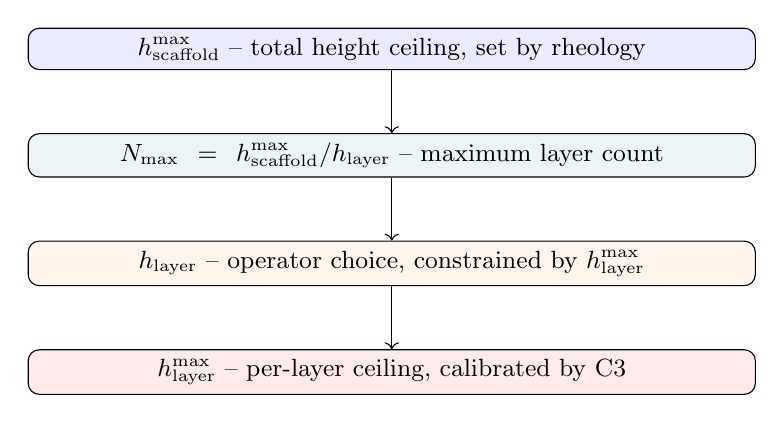
\begin{tikzpicture}[node distance=8mm,
    every node/.style={font=\small}]
  \node[draw, rounded corners, fill=blue!8, text width=9.0cm, align=center]
    (a) {$h_\mathrm{scaffold}^{\max}$ -- total height ceiling, set by rheology};
  \node[draw, rounded corners, fill=teal!8, text width=9.0cm, align=center,
        below=of a] (b)
    {$N_\mathrm{max}=h_\mathrm{scaffold}^{\max}/h_\mathrm{layer}$ -- maximum layer count};
  \node[draw, rounded corners, fill=orange!8, text width=9.0cm, align=center,
        below=of b] (c)
    {$h_\mathrm{layer}$ -- operator choice, constrained by $h_\mathrm{layer}^{\max}$};
  \node[draw, rounded corners, fill=red!8, text width=9.0cm, align=center,
        below=of c] (d)
    {$h_\mathrm{layer}^{\max}$ -- per-layer ceiling, calibrated by C3};
  \draw[->] (a) -- (b); \draw[->] (b) -- (c); \draw[->] (c) -- (d);
\end{tikzpicture}
\end{center}

\begin{intuitionbox}
$h_\mathrm{scaffold}^{\max}$ is about \emph{the whole stack}: can the
bottom layer hold everything above it? $h_\mathrm{layer}^{\max}$ is
about \emph{one layer}: does each fresh layer stay where I put it before
the next one arrives? They fail differently:
\begin{itemize}[leftmargin=1.4em,itemsep=1pt]
\item Exceeding $h_\mathrm{scaffold}^{\max}$: the tower bulges at the
  base and collapses outward.
\item Exceeding $h_\mathrm{layer}^{\max}$: each new layer sags into the
  previous one; the print proceeds but resolution is mushy.
\end{itemize}
\end{intuitionbox}

\subsection{Deriving $h_\mathrm{scaffold}^{\max}$}

\emph{Motivation.}
The formula $h^{\max}=\sigma_\mathrm{max}/(\rho g)$ follows from a
two-line free-body analysis.  Every number in Table~\ref{tab:hmax_three_criteria}
is a direct application of this single equation.

Per unit plan area, the bottom layer carries the weight of the column:
\begin{equation}
\sigma_\mathrm{stack}(N) = \rho\,g\,N\,h_\mathrm{layer}
                         = \rho\,g\,h_\mathrm{scaffold}.
\label{eq:sigma_stack}
\end{equation}
For the bottom layer to survive, $\sigma_\mathrm{stack}$ must remain
below the material's effective strength $\sigma_\mathrm{max}$:
\begin{equation}
\boxed{\,h_\mathrm{scaffold}^{\max}
 \;=\; \frac{\sigma_\mathrm{max}}{\rho\,g}\,}
\label{eq:hmax_master}
\end{equation}
with $\rho\approx 1000\,\si{\kg\per\m^3}$ and $g=9.81\,\si{\m/\s^2}$.
$h_\mathrm{layer}$ does \emph{not} appear here: the height ceiling is
independent of how thinly you slice.

\begin{derivationbox}[title={DERIVATION --- Self-weight force balance
for $h_\mathrm{scaffold}^{\max}$}]

\noindent\textbf{System and assumptions.}
Consider a prismatic column of deposited material with uniform
cross-sectional area $A$ and total height $h$.  The column stands
vertically in a gravitational field $g$.  We make three assumptions:
\begin{enumerate}[leftmargin=1.8em,itemsep=1pt]
  \item The cross-section is uniform from base to top (constant $A$).
  \item Loading is quasi-static: inertia and dynamic vibration are
    negligible.
  \item Inter-layer adhesion is neglected (conservative): each layer is
    treated as a fresh deposit bearing only the weight above it.
\end{enumerate}

\medskip\noindent\textbf{Step 1 --- Weight of material above the base.}
The total mass of the column is $m=\rho\,A\,h$.  Its weight is
\begin{equation}
W \;=\; m\,g \;=\; \rho\,g\,A\,h.
\end{equation}

\medskip\noindent\textbf{Step 2 --- Compressive stress at the base.}
This weight acts over the base area $A$.  The resulting compressive
(normal) stress at the base is
\begin{equation}
\sigma_\mathrm{base}
\;=\; \frac{W}{A}
\;=\; \frac{\rho\,g\,A\,h}{A}
\;=\; \rho\,g\,h.
\end{equation}
Note that $A$ cancels: the stress depends only on height and density,
not on the footprint size.

\medskip\noindent\textbf{Step 3 --- Yield condition.}
The base retains its shape while $\sigma_\mathrm{base}\leq\sigma_\mathrm{max}$,
where $\sigma_\mathrm{max}$ is the effective yield strength of the
deposited material.  Failure (base yielding $\to$ lateral slump) is
imminent when equality holds:
\begin{equation}
\rho\,g\,h^{\max} \;=\; \sigma_\mathrm{max}.
\end{equation}

\medskip\noindent\textbf{Step 4 --- Solve for $h^{\max}$.}
Dividing both sides by $\rho g$:
\begin{equation}
h_\mathrm{scaffold}^{\max}
\;=\; \frac{\sigma_\mathrm{max}}{\rho\,g}.
\tag{\ref{eq:hmax_master}}
\end{equation}
This is Eq.~\eqref{eq:hmax_master}.  The result is exact under the three
assumptions above; it does not involve $h_\mathrm{layer}$, confirming
that the total height ceiling is a \emph{material property divided by a
gravitational scale}, not a slicer parameter.

\medskip\noindent\textbf{Connection to $N$ layers.}
With $N$ layers of height $h_\mathrm{layer}$ each,
$h_\mathrm{scaffold}=N\,h_\mathrm{layer}$.  Substituting into the yield
condition gives
\begin{equation}
N_\mathrm{max}
\;=\; \frac{h_\mathrm{scaffold}^{\max}}{h_\mathrm{layer}}
\;=\; \frac{\sigma_\mathrm{max}}{\rho\,g\,h_\mathrm{layer}},
\end{equation}
consistent with Eq.~\eqref{eq:sigma_stack}: $N$ appears in the stress
but cancels in the final bound once we express everything in terms of
the total height $h_\mathrm{scaffold}=N\,h_\mathrm{layer}$.
\end{derivationbox}

\subsection{What is $\sigma_\mathrm{max}$? Three criteria}
\label{sec:three_criteria}

\emph{Motivation.}
The formula (Eq.~\ref{eq:hmax_master}) is exact once $\sigma_\mathrm{max}$
is known, but a fresh bioink has no sharp yield point --- it is a
viscoelastic gel whose apparent strength depends on the timescale of
loading.  We therefore define three SAOS-derived criteria, each
appropriate for a different print timescale, and cross-reference them to
the yield-stress determination methods derived in
Sec.~\ref{sec:rheo_primer} (Eq.~\ref{eq:yield_proxy} and the three ways
to measure $\tau_y$ listed there).

We estimate $\sigma_\mathrm{max}$ from SAOS data via three criteria,
each appropriate for a different print timescale.

\paragraph{Criterion (A) -- LVR endpoint (most permissive for short prints).}
\begin{equation}
\sigma_\mathrm{max}^{(A)} = G'_\mathrm{LVR}\,\gamma_\mathrm{LVR}.
\label{eq:sigmaA}
\end{equation}
This is exactly the oscillatory yield-stress proxy of
Eq.~\eqref{eq:yield_proxy}: the elastic stress stored in the network at
the end of the linear viscoelastic regime.  It assumes the bottom layer
never leaves the linear regime before it has to support additional
layers.  \emph{Most permissive} (largest $\sigma_\mathrm{max}$) for
inks with a wide LVR.  Appropriate for short-dwell prints where stacking
events are brief ($\lesssim\SI{1}{\s}$/layer).

\paragraph{Criterion (B) -- $G'(\omega=1\,\si{\radian\per\s})$ (literature default).}
\begin{equation}
\sigma_\mathrm{max}^{(B)} = G'(\omega=1\,\si{\radian\per\s}).
\label{eq:sigmaB}
\end{equation}
The literature default \citep{PaxtonEtAl2017, SchwabEtAl2020}.
At $\omega=1\,\si{\radian\per\s}$ the frequency sweep probes dynamics
on a timescale of $\sim\SI{1}{\s}$, matching the typical inter-layer
dwell time.  \emph{Intermediate} criterion.  Appropriate for typical
multi-layer DIW where dwell time is 1--10\,\si{\s} per layer.

\paragraph{Criterion (C) -- $G'(\omega=0.01\,\si{\radian\per\s})$ (most conservative).}
\begin{equation}
\sigma_\mathrm{max}^{(C)} = G'(\omega=0.01\,\si{\radian\per\s}),
\label{eq:sigmaC}
\end{equation}
obtained by power-law extrapolation $G'(\omega)=G'_0\,\omega^\beta$.
\emph{Most conservative}: it probes the gel stiffness at long timescales
($\sim\SI{100}{\s}$), where a critical-gel network has lost much of its
modulus.  Appropriate for slow prints or prints with crosslinking /
cell-loading pauses where dwell exceeds $\sim 100\,\si{\s}$.

\paragraph{Which criterion to report.}
The correct choice depends on the dwell time per layer.  For a given
$v_\mathrm{print}$ and footprint perimeter $P$, dwell time
$\approx P/v_\mathrm{print}$; match this to the $\omega$-scale
($\omega=2\pi/t_\mathrm{dwell}$) and use the criterion whose frequency
is closest.  Always report \emph{all three} in the manuscript and state
which controlled the experiment (see DR~6.1).

\paragraph{Low-$\omega$ gel character.}
The slope $\beta=d\ln G'/d\ln\omega$ (Winter--Chambon framework
\citealt{WinterChambon1987}) diagnoses network permanence:
\begin{itemize}[leftmargin=1.6em,itemsep=1pt]
\item $\beta\to 0$: true gel (permanent network); B $\approx$ C.
\item $\beta\approx 0.5$: critical gel (transient bonds); C $\ll$ B.
\item $\beta\to 1$: viscous liquid (no network).
\end{itemize}

\begin{examplebox}
Low-$\omega$ fit $G'(\omega)=G'_0\,\omega^\beta$:

\medskip\centering
\begin{tabular}{lccccc}
\toprule
Ink & $G'_0$ [\si{\Pa}] & $\beta$ [-] & $R^2$ & $G'(\omega=1)$ & $G'(\omega=0.01)$ \\
\midrule
C15           & 114.6 & 0.454 & 1.00 & 114.5 & 14.1  \\
C15 Gira 5.5  & 234.9 & 0.446 & 0.76 & 228.4 & 30.2  \\
Bozano        & 348.9 & 0.091 & 0.98 & 345.8 & 229.1 \\
\bottomrule
\end{tabular}

\medskip\flushleft
Bozano's $\beta=0.09$: true gel -- retains 66\% of its 1\,\si{\radian/s}
modulus down to 0.01\,\si{\radian/s}. C15 and NE have $\beta\approx
0.45$: critical-gel regime -- they lose modulus on long timescales.
Adding NE does not convert C15 to a true gel; it raises the modulus
while preserving the network type.
\end{examplebox}

\subsection{Three numbers per ink}

\emph{Motivation.}
Table~\ref{tab:hmax_three_criteria} translates the three $\sigma_\mathrm{max}$
criteria directly into millimetres via $h^{\max}=\sigma_\mathrm{max}/(\rho g)$.
The 10$\times$ spread within a single ink shows why print timescale must
be reported alongside every height claim.

\begin{table}[h]
\centering\small
\begin{tabular}{lcccccc}
\toprule
\multirow{2}{*}{Ink}
 & \multicolumn{2}{c}{(A) LVR endpoint}
 & \multicolumn{2}{c}{(B) $G'(\omega=1)$}
 & \multicolumn{2}{c}{(C) $G'(\omega=0.01)$} \\
\cmidrule(lr){2-3}\cmidrule(lr){4-5}\cmidrule(lr){6-7}
 & $\sigma$ [\si{\Pa}] & $h_\mathrm{max}$ [\si{\mm}]
 & $\sigma$ [\si{\Pa}] & $h_\mathrm{max}$ [\si{\mm}]
 & $\sigma$ [\si{\Pa}] & $h_\mathrm{max}$ [\si{\mm}] \\
\midrule
C15           & 172.9 & 17.6 & 114.5 & 11.7 & 14.1  & 1.4  \\
C15 Gira 5.5  & 558.5 & \textbf{56.9} & 228.4 & 23.3 & 30.2 & 3.1  \\
Bozano        & 47.6  & 4.9  & 345.8 & 35.3 & 229.1 & \textbf{23.4} \\
\bottomrule
\end{tabular}
\caption{Maximum scaffold height per ink under three SAOS-derived yield
criteria. Bold = the criterion that dominates in the most relevant print
regime.}
\label{tab:hmax_three_criteria}
\end{table}

\paragraph{Selection guide.}
\begin{itemize}[leftmargin=1.6em,itemsep=3pt]
\item \emph{Short-dwell prints ($\sim 1\,\si{\s}$/layer):} criterion (A).
  NE wins: \textbf{56.9\,\si{\mm}}.
\item \emph{Typical multi-layer DIW (1--10\,\si{\s}/layer):} criterion (B).
  Bozano wins: \textbf{35.3\,\si{\mm}}.
\item \emph{Slow prints ($>100\,\si{\s}$/layer):} criterion (C).
  Bozano wins decisively: \textbf{23.4\,\si{\mm}}.
\end{itemize}

\paragraph{The asymmetry between NE and Bozano.}
The NE has a wide LVR so its product $G'_\mathrm{LVR}\cdot\gamma_\mathrm{LVR}$
is large -- it wins criterion (A). But its transient network loses modulus
at long timescales -- it loses (B) and (C). Bozano's narrow LVR means
it loses (A), but its permanent bonds retain modulus -- it wins (B) and
(C). Neither dominates the other at every timescale: for the manuscript,
the NE is the better short-print ink; Bozano is the better long-print
ink.

\begin{inpracticebox}
\textbf{Pre-print height check in three steps.}
Before committing to a multi-layer print:
\begin{enumerate}[leftmargin=1.8em,itemsep=2pt]
\item \textbf{Estimate dwell time.} For a footprint perimeter $P$ printed
  at $v_\mathrm{print}$, one layer takes $t_\mathrm{dwell}\approx P/v_\mathrm{print}$.
  Example: $P=4\,\si{cm}$ at $v=8\,\mms$ $\Rightarrow$ $t\approx\SI{5}{\s}$
  $\Rightarrow$ use criterion~(B).
\item \textbf{Read $\sigma_\mathrm{max}$ from the SAOS output} (Table~\ref{tab:hmax_three_criteria}
  or from the extract script).  Apply Eq.~\eqref{eq:sigmaA},
  \eqref{eq:sigmaB}, or \eqref{eq:sigmaC} as appropriate.
\item \textbf{Compute $h^{\max}=\sigma_\mathrm{max}/(\rho g)$} and compare
  to the target scaffold height.
  \begin{itemize}[leftmargin=1.2em,itemsep=1pt]
  \item Target $\leq 50\%$ of $h^{\max}$: safe zone.
  \item $50\%$--$85\%$: feasible but validate in calibration test C4.
  \item $>85\%$: expect base bulging; reduce $N$ or switch to a
    stiffer ink.
  \end{itemize}
\end{enumerate}
For lattice scaffolds, additionally compute the Smay bound
(Eq.~\ref{eq:smay}); the smaller of the two controls.
\end{inpracticebox}

\subsection{Lattices and unsupported spans -- the Smay criterion}

\emph{Motivation.}
A solid tower and a lattice scaffold of the same ink share the same
$h^{\max}$ from Eq.~\eqref{eq:hmax_master} --- but a lattice has a
second failure mode: the unsupported struts spanning the pores can bend
and buckle under the weight of the layers above.  This constraint is
usually \emph{more restrictive} than the stacking bound and must be
checked for every lattice design.

For lattice scaffolds with unsupported strut spans of length $L$,
gravity-driven bending intervenes earlier than the stacking bound.
The Smay criterion \citep{HabibKhoda2018}:
\begin{equation}
h_\mathrm{max}(L) = \sqrt{\frac{1.94\,G'}{\rho g}}\cdot\sqrt{L}.
\label{eq:smay}
\end{equation}

\begin{derivationbox}[title={DERIVATION --- Beam-bending basis of the Smay criterion}]
\noindent\textbf{Setup.}
Model a single spanning strut as a simply-supported elastic beam of
circular cross-section (diameter $d$, the deposited filament width) and
length $L$ (the pore span).  The strut supports a distributed load from
the $N$ layers printed above it; the effective line load (force per unit
strut length) is
\begin{equation}
w \;=\; \rho\,g\,h_\mathrm{scaffold}\,d,
\end{equation}
where $d$ is the strut width (the load-bearing projection of the
layer-stack per unit span length) and $h_\mathrm{scaffold}=N h_\mathrm{layer}$.

\medskip\noindent\textbf{Step 1 --- Cross-section geometry.}
For a circular beam of diameter $d$:
\begin{align}
A &= \frac{\pi d^2}{4}, &
I &= \frac{\pi d^4}{64}, &
c &= \frac{d}{2}.
\end{align}

\medskip\noindent\textbf{Step 2 --- Maximum bending moment.}
For a uniformly loaded simply-supported beam (distributed load $w$ per
unit length, span $L$), the mid-span bending moment is
\begin{equation}
M_\mathrm{mid} \;=\; \frac{w\,L^2}{8}
             \;=\; \frac{\rho\,g\,h_\mathrm{scaffold}\,d\,L^2}{8}.
\end{equation}

\medskip\noindent\textbf{Step 3 --- Maximum bending stress at mid-span.}
Using the flexure formula $\sigma=Mc/I$:
\begin{equation}
\sigma_\mathrm{mid}
\;=\; \frac{M_\mathrm{mid}\,c}{I}
\;=\; \frac{\dfrac{\rho g h d L^2}{8}\cdot\dfrac{d}{2}}{\dfrac{\pi d^4}{64}}
\;=\; \frac{\rho g h L^2}{8} \cdot \frac{d^2/2}{\pi d^4/64}
\;=\; \frac{\rho g h L^2}{8} \cdot \frac{64}{2\pi d^2}
\;=\; \frac{4\,\rho\,g\,h\,L^2}{\pi\,d^2}.
\end{equation}

\medskip\noindent\textbf{Step 4 --- Yield condition.}
The strut survives while $\sigma_\mathrm{mid}\leq G'$ (using the storage
modulus $G'$ as the effective elastic modulus at the relevant timescale,
consistent with the $h^{\max}$ criteria above):
\begin{equation}
\frac{4\,\rho\,g\,h^{\max}\,L^2}{\pi\,d^2}
\;=\; G'.
\end{equation}
Solving for $h^{\max}$:
\begin{equation}
h^{\max}_\mathrm{beam}
\;=\; \frac{\pi\,d^2\,G'}{4\,\rho\,g\,L^2}.
\label{eq:hmax_beam_raw}
\end{equation}
This \emph{stress-based} bound gives $h^{\max}_\mathrm{beam}\propto d^2/L^2$:
stronger (larger $G'$) or wider ($d$) struts resist larger spans;
increasing $L$ reduces the allowable height quadratically.

\medskip\noindent\textbf{Step 5 --- The Smay semi-empirical form.}
In robocasting practice the critical quantity is not a single filament
diameter but the \emph{lattice periodicity}: the span $L$ is the
centre-to-centre distance between adjacent supporting struts, while the
effective load-bearing width scales with the lattice fill fraction.
Smay \citep{HabibKhoda2018} calibrated the bending and buckling
criterion across a range of inks and lattice geometries and obtained
the semi-empirical result
\begin{equation}
h_\mathrm{max}(L) \;=\; \sqrt{\frac{1.94\,G'}{\rho g}}\cdot\sqrt{L},
\tag{\ref{eq:smay}}
\end{equation}
where the coefficient $1.94$ absorbs the lattice geometry and boundary
conditions and $L$ enters as $\sqrt{L}$ (not $1/L^2$) because the
dominant failure mode in practice involves deflection-limited buckling
of the lattice network, not pure fibre bending.
Eq.~\eqref{eq:smay} is therefore presented as an empirically validated
correlation; Eq.~\eqref{eq:hmax_beam_raw} provides the \emph{physical
basis} (bending-stress scaling) from which it derives.

\medskip\noindent\textbf{Inverted form -- maximum allowable span.}
Squaring and rearranging Eq.~\eqref{eq:smay}:
\begin{equation}
h_\mathrm{max}^2 \;=\; \frac{1.94\,G'\,L}{\rho g}
\quad\Rightarrow\quad
L_\mathrm{max}
\;=\; \frac{h_\mathrm{target}^2\,\rho\,g}{1.94\,G'}.
\label{eq:smay_Lmax}
\end{equation}
Given a target scaffold height and a measured $G'$, $L_\mathrm{max}$ is
the largest lattice pore that will not collapse under self-weight before
reaching that height.
\end{derivationbox}

\begin{examplebox}
Buckling-corrected $h_\mathrm{max}$ at $L=1\,\si{\mm}$:

\medskip\centering
\begin{tabular}{lc}
\toprule
Ink & $h_\mathrm{max}(L=1\,\si{\mm})$ [\si{\mm}] \\
\midrule
C15           & 4.76 \\
C15 Gira 5.5  & 6.72 \\
Bozano        & 8.27 \\
\bottomrule
\end{tabular}

\medskip\flushleft
Even the NE, which can stack to $\sim 57\,\si{\mm}$ as a solid tower,
drops to $\sim 6.7\,\si{\mm}$ for a 1-\si{\mm} lattice span. For
lattice scaffolds, the Smay bound is usually the binding constraint.
\end{examplebox}

\begin{runningbox}{RUNNING EXAMPLE -- Solution to Q5}
\textbf{Question.} Will Ana's $1\times 1\times 2$\,cm$^3$ block survive
its own weight?

\medskip From Table~\ref{tab:hmax_three_criteria}, C15 Gira 5.5:
\begin{itemize}[leftmargin=1.4em,itemsep=1pt]
\item (A) $h_\mathrm{max}=56.9\,\si{\mm}$: block at 35\% of bound. Easy.
\item (B) $h_\mathrm{max}=23.3\,\si{\mm}$: block at 86\% of bound. Tight.
\item (C) $h_\mathrm{max}=3.1\,\si{\mm}$: block would collapse at this
  criterion.
\end{itemize}
\textbf{Which criterion applies?} At $v_\mathrm{print}=8\,\mms$ on a
$1\times 1\,\si{cm^2}$ footprint, layer time $\sim 1$--$2\,\si{\s}$:
criterion \textbf{(B) controls}.

\textbf{Verdict.} Feasible but close to the limit. Use
$h_\mathrm{layer}=0.36\,\si{\mm}$, $N=56$ layers to reach 20\,\si{\mm}
(86\% of the (B) bound). Validate in C4.

\medskip\emph{Still unknown:} the Wednesday calibration schedule. Q6.
\end{runningbox}

\begin{goingdeeperbox}
\textbf{Why criterion (A) can exceed criterion (B) for some inks.}
Criterion (A) is $\sigma^{(A)}=G'_\mathrm{LVR}\,\gamma_\mathrm{LVR}$;
criterion (B) is $\sigma^{(B)}=G'(\omega=1)$.  For a critical-gel ink
with $\beta\approx 0.45$ (e.g.\ the NE), $G'_\mathrm{LVR}$ (measured at
$\omega=10\,\si{\radian\per\s}$ in the amplitude sweep, a fast probe) is
several times larger than $G'(\omega=1)$.  Multiplying by the wide LVR
strain ($\sim 60\%$) gives $\sigma^{(A)}\gg\sigma^{(B)}$.  Criterion (A)
is therefore \emph{not} always conservative: it is the correct bound when
loading is genuinely fast (sub-second dwell), but it over-predicts
stability for slower prints.  This is why all three criteria are required
and the dwell-time argument must accompany every quoted $h^{\max}$.
\end{goingdeeperbox}

% ---- Exercises ----
\medskip\noindent\textbf{Exercises.}

\begin{exercise}{\diffA}
A bioink for the C15 Gira~5.5 formulation gives an amplitude-sweep LVR
plateau $G'_\mathrm{LVR}=\SI{916}{\Pa}$ and critical strain
$\gamma_\mathrm{LVR}=\SI{0.609}{}$ (absolute).  Using criterion (A) and
the master formula Eq.~\eqref{eq:hmax_master} with $\rho=\SI{1000}{\kg\per\m^3}$
and $g=\SI{9.81}{\m\per\s^2}$:
\begin{enumerate}[label=(\alph*),leftmargin=1.8em,itemsep=2pt]
\item Calculate $\sigma_\mathrm{max}^{(A)}$.
\item Calculate $h_\mathrm{scaffold}^{\max}$ in \si{\mm}.
\end{enumerate}
\end{exercise}
\begin{solution}
(a) $\sigma_\mathrm{max}^{(A)} = G'_\mathrm{LVR}\,\gamma_\mathrm{LVR}
= 916\times0.609 = \SI{557.9}{\Pa}\approx\SI{558.5}{\Pa}$
(table rounding; use $\SI{558.5}{\Pa}$ to match Table~\ref{tab:hmax_three_criteria}).

(b) $h_\mathrm{scaffold}^{\max}=\sigma_\mathrm{max}/(\rho g)
= 558.5/(1000\times9.81)
= 558.5/9810
= 0.05693\,\si{\m}
= \mathbf{56.9\,\si{\mm}}$ (matches Table~\ref{tab:hmax_three_criteria} exactly).

\textit{Check units:} $[\si{\Pa}]/[\si{\kg\per\m^3}\cdot\si{\m\per\s^2}]
= [\si{\N\per\m^2}]/[\si{\kg\per\m^2\per\s^2}]
= [\si{\m}]$.  Correct.
\end{solution}

\begin{exercise}{\diffB}
Using Table~\ref{tab:hmax_three_criteria}, compare $h_\mathrm{max}$ under
criteria (A) and (B) for the Bozano ink.
\begin{enumerate}[label=(\alph*),leftmargin=1.8em,itemsep=2pt]
\item State the two $\sigma_\mathrm{max}$ values and the resulting heights.
\item Explain the physical reason one criterion gives a larger height.
\item Which criterion is \emph{conservative} (i.e.\ gives the safer,
  lower height bound) and under what print conditions?
\end{enumerate}
\end{exercise}
\begin{solution}
(a) Criterion (A): $\sigma^{(A)}=\SI{47.6}{\Pa}$,
$h^{\max}_{(A)}=47.6/9810=0.00485\,\si{\m}\approx\SI{4.9}{\mm}$.
Criterion (B): $\sigma^{(B)}=\SI{345.8}{\Pa}$,
$h^{\max}_{(B)}=345.8/9810=0.03525\,\si{\m}\approx\SI{35.2}{\mm}$.
Ratio: $\sigma^{(B)}/\sigma^{(A)}\approx7.3\times$.

(b) Bozano has a \emph{narrow} LVR ($\gamma_\mathrm{LVR}=13.7\%$), so
the product $G'_\mathrm{LVR}\,\gamma_\mathrm{LVR}$ is small despite a
high plateau modulus.  Criterion (A) therefore gives a low
$\sigma^{(A)}$.  However, Bozano is a true gel ($\beta=0.091$): its
$G'$ is nearly flat across the frequency spectrum, so
$G'(\omega=1)\approx G'_\mathrm{LVR}=\SI{346}{\Pa}$, and criterion (B)
returns a much larger bound.

(c) Criterion (A) is conservative for \emph{fast prints} ($\lesssim\SI{1}{\s}$/layer)
because it uses only the elastic energy the gel can store before
microstructure damage.  For the Bozano ink specifically, (A) is the
\emph{most conservative} choice at any timescale; criterion (B) is the
correct bound for typical DIW dwell times (1--10\,\si{\s}/layer).
\end{solution}

\begin{exercise}{\diffC}
A lattice scaffold of C15 Gira~5.5 ink is designed with a target
height of $h_\mathrm{target}=\SI{20}{\mm}$ and a regular square-pore
lattice.  Using the inverted Smay formula (Eq.~\eqref{eq:smay_Lmax})
with $G'=G'(\omega=1\,\si{\radian\per\s})=\SI{228.4}{\Pa}$,
$\rho=\SI{1000}{\kg\per\m^3}$, $g=\SI{9.81}{\m\per\s^2}$:
\begin{enumerate}[label=(\alph*),leftmargin=1.8em,itemsep=2pt]
\item Compute $L_\mathrm{max}$, the largest lattice pore span that allows
  the scaffold to reach $h_\mathrm{target}$ without strut collapse.
\item Verify by plugging $L_\mathrm{max}$ back into Eq.~\eqref{eq:smay}
  and confirming that $h_\mathrm{max}(L_\mathrm{max})=\SI{20}{\mm}$.
\item If the designer wants a $\SI{1}{\mm}$ pore, what is the maximum
  printable height?
\end{enumerate}
\end{exercise}
\begin{solution}
(a) From Eq.~\eqref{eq:smay_Lmax}:
\begin{align}
L_\mathrm{max}
&= \frac{h_\mathrm{target}^2\,\rho\,g}{1.94\,G'} \notag\\
&= \frac{(0.020)^2\times1000\times9.81}{1.94\times228.4} \notag\\
&= \frac{4.000\times10^{-4}\times9810}{443.1} \notag\\
&= \frac{3.924}{443.1}
= 8.86\times10^{-3}\,\si{\m}
= \mathbf{8.86\,\si{\mm}}.
\end{align}

(b) Check with Eq.~\eqref{eq:smay}:
\begin{align}
h_\mathrm{max}(L_\mathrm{max})
&= \sqrt{\frac{1.94\times228.4}{1000\times9.81}}\cdot\sqrt{8.86\times10^{-3}} \notag\\
&= \sqrt{0.04517}\cdot\sqrt{8.86\times10^{-3}} \notag\\
&= 0.2125\times0.09413
= 0.02000\,\si{\m}
= \mathbf{20.0\,\si{\mm}}.\ \checkmark
\end{align}

(c) At $L=\SI{1}{\mm}=\SI{e-3}{\m}$:
\begin{align}
h_\mathrm{max}
&= \sqrt{\frac{1.94\times228.4}{9810}}\cdot\sqrt{10^{-3}} \notag\\
&= 0.2125\times0.03162
= 6.72\times10^{-3}\,\si{\m}
= \mathbf{6.72\,\si{\mm}},
\end{align}
consistent with Table~\ref{tab:hmax_three_criteria}.  The designer must
either use a smaller pore ($L<\SI{8.86}{\mm}$ for a $\SI{20}{\mm}$
tower) or switch to a stiffer ink to support the $\SI{1}{\mm}$ pore at
that height.
\end{solution}

\begin{takeawaybox}
\begin{itemize}[leftmargin=1.4em,itemsep=2pt]
\item $h_\mathrm{scaffold}^{\max}=\sigma_\mathrm{max}/(\rho g)$:
  layer thickness does not appear -- slicing into thinner layers does
  not change the height ceiling.
\item The three SAOS criteria span a 10$\times$ range; print timescale
  selects which applies.  Always report all three in the manuscript.
\item Criterion (A) uses the yield proxy of Eq.~\eqref{eq:yield_proxy}
  directly; criteria (B) and (C) use the frequency sweep and are more
  conservative for inks with transient networks ($\beta\approx0.45$).
\item Lattice geometry (Smay) is usually the binding constraint for
  scaffold prints with unsupported spans; use the inverted form
  (Eq.~\ref{eq:smay_Lmax}) to design pore size for a target height.
\end{itemize}
\end{takeawaybox}

\begin{designrulebox}
\textbf{DR 6.1.} Always compute and report all three height criteria.
The manuscript should explain which criterion controlled the experiment
and why (dwell time argument).

\textbf{DR 6.2.} For lattice designs, compute the Smay bound for the
intended strut span before committing to an ink. Even a high-$G'$ ink
may fail at mm-scale spans.

\textbf{DR 6.3.} Validate $h_\mathrm{scaffold}^{\max}$ experimentally
in C4 and record which SAOS criterion best matches the observed
collapse onset. Use that criterion for all future prints of that ink
at similar dwell times.

\textbf{DR 6.4.} Before every multi-layer print, run the three-step
pre-print check (see the \textsc{In Practice} box above).  If the
target height exceeds 85\% of the applicable $h^{\max}$ criterion,
print a single-layer C4 slab first and verify dimensional fidelity.
\end{designrulebox}

% =================================================================
\section{Failure Morphology: Physical Causes and Corrective Actions}
\label{sec:failure}
\label{sec:failures}

This chapter catalogues the failure modes observed in DIW printing,
their physical origin in the rheological and hydraulic framework, and
the corrective actions available within this workflow. Every corrective
action targets $V_p$, $\mathrm{EM}_\mathrm{slicer}$, geometry, or
needle gauge -- never $\Delta P$ directly (it is an output, not a knob).

\subsection{Under-extrusion}

\begin{failurebox}{Under-extrusion ($d_\mathrm{fil}/\mathrm{ID}<0.9$)}
\textbf{Observation.} Filaments are thinner than the needle ID;
gaps appear between adjacent lines; poor adhesion between layers.

\textbf{Physical causes.}
\begin{itemize}[leftmargin=1.4em,itemsep=2pt]
\item $\mathrm{EM}_\mathrm{slicer}$ too low: slicer commands too little
  material per unit length.
\item Silent motor stalling: $\Delta P$ has exceeded motor stall torque;
  the piston is not advancing despite E-axis commands.
\item Clog or air bubble in the syringe or needle.
\item Slip between piston rubber and syringe wall ($f_\mathrm{slip}<1$).
\end{itemize}

\textbf{Rheological interpretation.} Low $R_\mathrm{rec}$ gives
$k_\mathrm{flow}<1$; if $\mathrm{EM}_\mathrm{slicer}$ was set to
$k_\mathrm{flow}$ instead of $1/k_\mathrm{flow}$, the error doubles.

\textbf{Corrective actions.}
\begin{enumerate}[leftmargin=1.6em,itemsep=1pt]
\item Raise $\mathrm{EM}_\mathrm{slicer}$ in steps of 0.05.
\item If no change: check predicted $\Delta P$ against motor capacity.
  If close to stall, lower $V_p$ by 25\% and switch to wider needle.
\item Purge the needle with slow extrusion; inspect for air.
\item Run C2 to measure $f_\mathrm{slip}$ directly.
\end{enumerate}
\end{failurebox}

\subsection{Over-extrusion}

\begin{failurebox}{Over-extrusion ($d_\mathrm{fil}/\mathrm{ID}>1.2$)}
\textbf{Observation.} Filaments are wider than expected; adjacent lines
merge; scaffold walls are rough; towers develop a barrel shape.

\textbf{Physical causes.}
\begin{itemize}[leftmargin=1.4em,itemsep=2pt]
\item $\mathrm{EM}_\mathrm{slicer}$ too high.
\item Die swell larger than predicted by the $m$-proxy; $\beta_\mathrm{swell}$
  underestimated.
\item $V_p$ too high relative to the XY feedrate ($v_\mathrm{print}$ too slow).
\end{itemize}

\textbf{Corrective actions.}
\begin{enumerate}[leftmargin=1.6em,itemsep=1pt]
\item Decrease $\mathrm{EM}_\mathrm{slicer}$ in steps of 0.05.
\item If $\mathrm{EM}$ is already $\leq 1$, reduce $V_p$ by 25\%.
\item Measure die swell directly in C1 and update $\beta_\mathrm{swell}$.
\end{enumerate}
\end{failurebox}

\subsection{Die swell excess}

\begin{failurebox}{Filament always wider than needle ID even at low $V_p$}
\textbf{Physical cause.} High stored elastic energy (low $m$ in Cross
model or high $n$ in Power Law). The $m$-based proxy
($\beta\approx 0.3(1-m)$) may underestimate swell for strongly
viscoelastic inks.

\textbf{Rheological interpretation.} High $\De$ at exit ($t_\mathrm{relax}
\gg R_n/\bar v_n$): the material exits before it has time to deform
viscously; the stored elastic strain releases as radial expansion.

\textbf{Corrective actions.}
\begin{enumerate}[leftmargin=1.6em,itemsep=1pt]
\item Measure $w_\mathrm{line}$ directly in C1 and use
  $\beta_\mathrm{swell}^\mathrm{exp}=w_\mathrm{line}/\mathrm{ID}-1$.
\item Use a longer needle (larger $L/R$): more time at constant flow
  means more viscous dissipation before exit.
\item Reduce $V_p$ to lower $\bar v_n$ and hence the Weissenberg number
  at exit.
\end{enumerate}
\end{failurebox}

\subsection{Scaffold collapse (base bulging)}

\begin{failurebox}{Base bulging / tower collapse}
\textbf{Observation.} The printed object bulges or splays outward from
the base as layer count increases.

\textbf{Physical cause.} $\sigma_\mathrm{stack}$ has exceeded
$\sigma_\mathrm{max}$ at the print's effective timescale.

\textbf{Rheological interpretation.} The controlling SAOS criterion
has been exceeded. If layer dwell is $\sim 1\,\si{\s}$, criterion (B)
controls; if $>100\,\si{\s}$, criterion (C) controls. The NE ink is
particularly susceptible on slow prints because $G'(\omega=0.01)=30\,\si{\Pa}$
predicts $h_\mathrm{max}=3.1\,\si{\mm}$ under criterion (C).

\textbf{Corrective actions.}
\begin{enumerate}[leftmargin=1.6em,itemsep=1pt]
\item Reduce $N$ to stay under the controlling height criterion.
\item Increase $v_\mathrm{print}$ to shorten dwell, shifting the
  controlling criterion from (C) toward (B) or (A).
\item Switch to a higher-modulus ink: Bozano for long-dwell prints;
  NE for short-dwell.
\end{enumerate}
\end{failurebox}

\subsection{Lattice strut buckling}

\begin{failurebox}{Mid-span sag of bridging filaments}
\textbf{Physical cause.} Smay buckling: the unsupported span $L$ is
too long for the ink's $G'$.

\textbf{Corrective actions.}
\begin{enumerate}[leftmargin=1.6em,itemsep=1pt]
\item Shorten strut span (reduce cell size).
\item Switch to a higher-$G'$ ink (e.g.\ Bozano).
\item Increase $G'_\mathrm{LVR}$ by adding crosslinker or increasing
  polymer concentration.
\end{enumerate}
\end{failurebox}

\subsection{Intermittent extrusion (motor skip)}

\begin{failurebox}{Intermittent flow / motor skip}
\textbf{Observation.} Filament diameter oscillates; audible clicking
from the motor; E-axis step count diverges from actual piston position.

\textbf{Physical cause.} Predicted $\Delta P$ periodically exceeds motor
stall torque, particularly at turns and during acceleration.

\textbf{Corrective actions.}
\begin{enumerate}[leftmargin=1.6em,itemsep=1pt]
\item Lower $V_p$ by 25\%. Re-check $\Delta P$ from CSV.
\item Switch to wider needle (e.g.\ 21G $\to$ 18G).
\item Increase acceleration settling time in firmware (add dwell at corners).
\end{enumerate}
\end{failurebox}

\subsection{Layer-by-layer fusion (loss of resolution)}

\begin{failurebox}{Adjacent layers merge; scaffold is mushy}
\textbf{Physical cause.} Insufficient recovery between deposition
events ($h_\mathrm{layer}^{\max}$ exceeded, or $R_\mathrm{rec}$ too
low for the layer dwell).

\textbf{Corrective actions.}
\begin{enumerate}[leftmargin=1.6em,itemsep=1pt]
\item Decrease $h_\mathrm{layer}$ to stay within the C3-validated
  $h_\mathrm{layer}^{\max}$.
\item Increase $v_\mathrm{travel}$ (non-extrusion move speed) to give
  the just-deposited layer more time to recover before the next pass.
\item Increase line spacing; reduce infill density.
\item Switch to an ink with higher $R_\mathrm{rec}$ (Bozano).
\end{enumerate}
\end{failurebox}

\subsection{Stringing during travel}

\begin{failurebox}{Ink trails during non-extrusion moves}
\textbf{Physical cause.} Recovery too slow at travel timescale; the
ink at the nozzle tip remains mobile during XY travel.

\textbf{Note.} DIW slicers typically do not support retraction
(reversing the piston to pull back ink). Attempting retraction with
a piston printer causes a pressure deficit that takes many mm of
subsequent extrusion to recover -- producing a dead zone.

\textbf{Corrective actions.}
\begin{enumerate}[leftmargin=1.6em,itemsep=1pt]
\item Ensure retraction is set to \textbf{zero} in the slicer.
\item Increase $v_\mathrm{travel}$ to spend less time dragging the
  nozzle over the substrate.
\item If stringing persists, raise $V_p$ slightly to increase the
  viscosity at low $\gd$ (by raising the mean shear rate in the needle)
  -- counterintuitive but sometimes effective.
\end{enumerate}
\end{failurebox}

\subsection{Rough filament surface / extrudate distortion}

\begin{failurebox}{Rough, wavy, or distorted filament surface}
\textbf{Physical cause.} Elastic instability (``die melt fracture'' analogue for
gels): the Weissenberg number at the needle exit is high enough
that the stored elastic energy releases as surface corrugations rather
than smooth radial expansion.

\textbf{Corrective actions.}
\begin{enumerate}[leftmargin=1.6em,itemsep=1pt]
\item Reduce $V_p$ to lower the Weissenberg number.
\item Use a longer needle to increase viscous dissipation before exit.
\item If the ink is new, check whether $\eta_\infty$ is very low --
  a near-zero high-shear plateau makes the exit transition sharp and
  prone to instability.
\end{enumerate}
\end{failurebox}

\begin{takeawaybox}
\begin{itemize}[leftmargin=1.4em,itemsep=2pt]
\item Every failure mode has a rheological root cause. Diagnose from
  the parameter tables before adjusting hardware.
\item The most common single error is typing $k_\mathrm{flow}$ into
  the slicer instead of $1/k_\mathrm{flow}$ -- produces immediate
  severe under-extrusion.
\item Motor skip at corners is the second most common; always check
  predicted $\Delta P$ against motor capacity before the first print.
\item Never use retraction on a piston DIW printer.
\end{itemize}
\end{takeawaybox}

\begin{designrulebox}
\textbf{DR 7.1.} Diagnose failure morphology \emph{before} adjusting
the slicer blindly. Every symptom maps to exactly one physical cause in
this chapter.

\textbf{DR 7.2.} Run C1 (filament width sweep) before C2--C4 on any
new ink. C1 reveals under/over-extrusion and die swell simultaneously
-- it is the cheapest diagnostic.

\textbf{DR 7.3.} Keep a photographic log of every calibration session.
Failure modes are much faster to diagnose when you can compare
current vs.\ previous prints side-by-side.
\end{designrulebox}

\bigskip\hrule\bigskip

% =================================================================
% PART II -- INKS AND INSTRUMENTS
% =================================================================
\part*{Part II -- Inks and Instruments}
\addcontentsline{toc}{part}{Part II -- Inks and Instruments}

% =================================================================
\section{The Three Project Inks}
\label{sec:inks}

\subsection{C15 -- CMC baseline}

\paragraph{Composition.} Carboxymethyl cellulose (CMC) in aqueous
buffer, formulation \texttt{C15}. Molecular weight characterised per
\citet{daSilva2018} -- \emph{this reference is mandatory in the
manuscript; peer review requires it for MW determination.}

\paragraph{Rheological character.} Critical-gel polymer solution
($\beta=0.454$). Pronounced shear thinning ($n_\mathrm{PL}=0.40$,
Cross $m=0.81$). Moderate rest viscosity ($\eta_0\approx 578\,\Pas$).
Wide linear regime ($\gamma_\mathrm{LVR}=64\%$). Moderate recovery
($\sim 60\%$ at deposition shear).

\paragraph{Printability profile.}
\begin{itemize}[leftmargin=1.4em,itemsep=2pt]
\item Pressure: \emph{moderate} ($\Delta P\approx 140\,\si{\kPa}$
  Cross at $V_p=0.01\,\mms$, 21G).
\item Wall shear: $\tau_w\approx 560\,\si{\Pa}$,
  $\gd_w\approx 220\,\si{\per\s}$ -- cell-safe with margin.
\item Scaffold height: modest (12\,\si{\mm} at criterion B).
\item Lattice strut bound: tightest of the three ($\sim 4.8\,\si{\mm}$
  at $L=1\,\si{\mm}$).
\item Extrusion Multiplier: $\mathrm{EM}\approx 1.17$.
\end{itemize}

\paragraph{Use case.} Reference / benchmark ink. The simplest
formulation; the baseline against which NE inclusion is compared.

\subsection{C15 Gira 5.5 -- CMC + sunflower-oil nanoemulsion (NE)}

\paragraph{Composition.} C15 base with statistically optimised
sunflower-oil nanoemulsion (project: \texttt{Statistical\_Analysis\_Consolidated},
\texttt{Qualify.tex}) incorporated as a filler.

\paragraph{Rheological character.} Critical-gel ($\beta=0.446$ --
microstructure preserved relative to C15). Sharply shear-thinning
($n_\mathrm{PL}=0.24$, Cross $m=0.988$). Quadrupled rest viscosity
($\eta_0\approx 2440\,\Pas$) and tripled LVR modulus
($G'_\mathrm{LVR}=916\,\si{\Pa}$) at \emph{unchanged}
$\gamma_\mathrm{LVR}\approx 61\%$. Slightly reduced recovery ($\sim 45\%$).

\paragraph{Printability profile.}
\begin{itemize}[leftmargin=1.4em,itemsep=2pt]
\item Pressure: modestly higher than C15 ($\Delta P\approx 165\,\si{\kPa}$).
\item Wall shear: \emph{lower} than C15 ($\tau_w\approx 660\,\si{\Pa}$,
  $\gd_w\approx 60\,\si{\per\s}$) -- sharper shear thinning.
\item Scaffold height: best under criterion A ($\sim 57\,\si{\mm}$);
  good under criterion B ($\sim 23\,\si{\mm}$).
\item Die swell: minimal ($\beta_\mathrm{swell}\approx 0.004$);
  cleanest predicted filament geometry.
\item Extrusion Multiplier: $\mathrm{EM}\approx 1.49$.
\end{itemize}

\paragraph{Use case.} The headline ink of this project. The NE acts
as a \emph{reinforcing filler}: it stiffens the network without
narrowing the LVR or changing the network type (preserved $\beta$,
preserved $\gamma_\mathrm{LVR}$). This is the printability advantage
to highlight in the manuscript -- the NE stiffens without embrittling.

\subsection{Bozano -- commercial hair gel}

\paragraph{Composition.} Commercial Bozano hair gel
(\texttt{Gel de Cabelo Bozano}) used as control.

\paragraph{Rheological character.} \emph{True gel}
($\beta=0.091$ -- the only true gel of the three). Sharply shear-thinning
($n_\mathrm{PL}=0.23$, Cross $m=0.866$). Very high $\eta_0\approx
6350\,\Pas$ with the slowest transition ($\lambda=73\,\si{\s}$).
Narrow LVR ($\gamma_\mathrm{LVR}=14\%$). Near-complete recovery ($\sim 98\%$
across all tested $\gd$).

\paragraph{Printability profile.}
\begin{itemize}[leftmargin=1.4em,itemsep=2pt]
\item Pressure: \emph{lowest} of the three ($\Delta P\approx 116\,\si{\kPa}$)
  -- long $\lambda$ puts the needle deep into the shear-thinned regime.
\item Wall shear: lowest ($\tau_w\approx 470\,\si{\Pa}$,
  $\gd_w\approx 8\,\si{\per\s}$) -- extremely benign to cells.
\item Scaffold height: loses on criterion A (4.8\,\si{\mm}, narrow LVR
  penalty) but wins on B (35\,\si{\mm}) and C (23\,\si{\mm}).
\item Extrusion Multiplier: $\mathrm{EM}\approx 0.93$ -- the only ink
  requiring a \emph{reduction} from nominal.
\end{itemize}

\paragraph{Use case.} Commercial benchmark. Sets the upper bar for
recovery and quasi-static stability; sets the lower bar for strain
tolerance (narrow LVR). Useful as a reference because it is routinely
printed on the lab DIW.

\paragraph{Comparative summary.}
\begin{center}\small
\begin{tabular}{lccc}
\toprule
Property & C15 & C15 Gira 5.5 & Bozano \\
\midrule
Network type & Critical gel & Critical gel & True gel \\
$\eta_0$ [\si{\Pa\s}] & 578 & 2440 & 6354 \\
$m$ (sharpness) & 0.81 & 0.99 & 0.87 \\
$G'_\mathrm{LVR}$ [\si{\Pa}] & 270 & 916 & 348 \\
$\gamma_\mathrm{LVR}$ [\%] & 64 & 61 & 14 \\
$R_\mathrm{rec}$ @ 100\,\si{\per\s} [\%] & 60 & 45 & 98 \\
$h_\mathrm{max}$ criterion B [\si{\mm}] & 12 & 23 & 35 \\
$\mathrm{EM}_\mathrm{slicer}$ & 1.17 & 1.49 & 0.93 \\
\bottomrule
\end{tabular}
\end{center}

% =================================================================
\section{Nanoemulsion Mechanics}
\label{sec:ne_mechanics}

This chapter explains the physical mechanisms by which the sunflower-oil
nanoemulsion modifies the CMC matrix. Understanding these mechanisms is
essential for interpreting the rheological results, designing improved
formulations, and framing the manuscript discussion correctly.

\subsection{Nanoemulsion structure and droplet characteristics}

The sunflower-oil nanoemulsion consists of oil droplets stabilised by
a surfactant shell dispersed in an aqueous continuous phase. Key
structural parameters:

\begin{itemize}[leftmargin=1.6em,itemsep=2pt]
\item \textbf{Droplet size} ($d$, nm): set by the homogenisation protocol
  and surfactant HLB value. Smaller droplets ($d<200\,\si{\nm}$) are
  kinetically stable and increase the effective particle volume fraction
  for a given oil loading.
\item \textbf{Volume fraction} ($\phi$): controls the magnitude of
  viscosity enhancement. At high $\phi$, droplets form a jammed network
  even without polymer bridging.
\item \textbf{Zeta potential}: determines electrostatic stability.
  Large negative $\zeta$ ($<-30\,\si{\mV}$) prevents droplet coalescence.
\end{itemize}

\subsection{How the NE stiffens the CMC matrix}

Three parallel mechanisms operate when the NE is incorporated into the
CMC gel:

\paragraph{Hydrodynamic reinforcement.} Rigid or semi-rigid droplets
(relative to the surrounding polymer) increase the effective viscosity
even without direct polymer-droplet bonds, following the Einstein
relation at dilute loading:
\begin{equation}
\eta_\mathrm{eff} \;\approx\; \eta_\mathrm{matrix}(1+2.5\phi).
\label{eq:einstein}
\end{equation}
At higher $\phi$, the Krieger-Dougherty expression replaces this with
a divergence near the jamming fraction $\phi_m$.

\paragraph{Polymer-droplet bridging.} CMC chains adsorb onto the
surfactant-coated oil surface. Each droplet effectively becomes a
transient crosslink node in the polymer network, increasing $G'$
without forming permanent covalent bonds (hence the preserved
$\gamma_\mathrm{LVR}$: a crosslinker would narrow the LVR, but
bridging via adsorption does not).

\paragraph{Lubrication at the macroscale.} During shear, the oil phase
acts as a lubricant between CMC chain bundles, lowering the critical
shear rate at which the macroscopic network yields. This is mechanistically
responsible for the sharper thinning exponent ($m=0.988$ for the NE
vs.\ $m=0.811$ for C15): the oil-mediated lubrication makes the
network-to-fluid transition more cooperative.

\subsection{Emulsion stability under shear}

During extrusion through the needle, the NE is exposed to
$\gd_w\approx 60\,\si{\per\s}$ for $L_n/\bar v_n\approx 0.05\,\si{\s}$.
Three potential instabilities must be assessed:

\begin{itemize}[leftmargin=1.6em,itemsep=2pt]
\item \textbf{Droplet deformation}: the capillary number
  $\Ca_d=\eta_\mathrm{matrix}\gd d/\sigma_\mathrm{NE}$ must be
  $<\Ca_d^\mathrm{crit}\approx 0.5$ for droplets to remain spherical.
  For $\eta_\mathrm{matrix}\sim 10\,\Pas$ (at $\gd_w=60\,\si{\per\s}$),
  $d=200\,\si{\nm}$, $\sigma_\mathrm{NE}\sim 5\,\si{\mN/\m}$:
  $\Ca_d\sim 0.02\ll 0.5$. Droplets remain spherical.
\item \textbf{Droplet coalescence}: time in the high-shear zone is
  short ($\sim 50\,\si{ms}$). Zeta potential $<-30\,\si{\mV}$ provides
  electrostatic protection. Coalescence risk: low.
\item \textbf{Ostwald ripening}: relevant only over hours to days in
  quiescent storage, not during printing. Mitigated by small droplet
  size and surfactant loading.
\end{itemize}

\textbf{Conclusion}: the NE is mechanically stable during extrusion at
the operating conditions of this project. No special pre-treatment or
post-deposition stabilisation is needed for acellular prints.

\subsection{Structural recovery enhancement mechanism}

The NE reduces $R_\mathrm{rec}$ relative to C15 (45\% vs.\ 60\% at
$100\,\si{\per\s}$). The mechanism is: after high-shear disruption,
the CMC chains must re-entangle and rebuild their network. Droplet
re-adsorption is slower than polymer re-entanglement, creating a
two-timescale recovery: a fast polymer phase (caught at 30\,\si{\s})
and a slower droplet-bridging phase (minutes). The 30-\si{\s}
measurement used for $R_\mathrm{rec}$ captures only the first phase.
This is why the bead spreads more than expected from the $G'_\mathrm{LVR}$
alone -- the slow recovery phase means the deposited bead is not as
stiff as its LVR modulus implies.

\textbf{Manuscript implication.} This two-timescale argument explains
why the NE requires a higher $\mathrm{EM}_\mathrm{slicer}$ despite its
higher $G'_\mathrm{LVR}$. Both must be reported and the mechanism
discussed.

\subsection{Carrier model rationale}

The NE serves as a drug carrier model for future pharmaceutical
loading (e.g.\ Amphotericin B). The oil core provides a hydrophobic
domain that sequesters lipophilic drugs; the surfactant shell controls
release kinetics and biocompatibility. For the current phase (acellular
scaffold printing), no drug is loaded -- the NE acts solely as a
rheological modifier and structural filler. Future work will characterise
the effect of drug loading on the rheological parameters described in
this document.

\begin{designrulebox}
\textbf{DR 9.1.} Always characterise both the emulsion alone and the
CMC+NE composite separately. Changes in droplet size upon mixing must
be verified by DLS.

\textbf{DR 9.2.} The preserved $\gamma_\mathrm{LVR}$ is the key
evidence that the NE acts as a filler rather than a crosslinker. This
interpretation must be defended explicitly in the manuscript against
reviewers who may suggest chemical crosslinking.

\textbf{DR 9.3.} When loading drugs into the NE, re-characterise
$\eta_0$, $G'_\mathrm{LVR}$, and $R_\mathrm{rec}$ -- drug molecules
can alter the polymer-droplet interfacial energy and change all three.
\end{designrulebox}

% =================================================================
\section{Rheological Tests: Instrument and Battery}
\label{sec:tests}

\subsection{Instrument}

Anton Paar MCR 501 stress-controlled rheometer. Plate--plate (PP25,
PP50) or cone--plate (CP50) tooling. Solvent trap to suppress
evaporation. Temperature $25\,^\circ$C unless noted. Data exported as
\texttt{.xls} (primary; \texttt{xlrd}-compatible -- do not use
\texttt{openpyxl}), \texttt{.txt} (human-readable), and \texttt{.tri}
(proprietary archive, do not alter).

\paragraph{Pre-experiment checklist.}
\begin{itemize}[leftmargin=1.4em,itemsep=1pt]
\item[$\square$] Verify instrument zero-gap calibration.
\item[$\square$] Check solvent trap seal; fill if needed.
\item[$\square$] Allow sample to equilibrate at $25\,^\circ$C for
  $\geq 10\,\si{\minute}$ before first measurement.
\item[$\square$] Load sample slowly (avoid air bubbles); trim cleanly.
\item[$\square$] Run a brief pre-shear at $\gd=10\,\si{\per\s}$ for
  30\,\si{\s} then wait 5\,\si{\minute} to erase loading history.
\end{itemize}

\paragraph{Post-experiment checklist.}
\begin{itemize}[leftmargin=1.4em,itemsep=1pt]
\item[$\square$] Export in all three formats; verify file sizes are
  non-zero.
\item[$\square$] Clean geometry with distilled water immediately;
  dry completely before storage.
\item[$\square$] Record batch ID, temperature, and gap in the lab notebook.
\end{itemize}

\subsection{Standard test battery}

\begin{table}[h]
\centering\small
\begin{tabular}{p{2.2cm} p{4.5cm} p{8.0cm}}
\toprule
\textbf{Test} & \textbf{What it measures} & \textbf{Protocol} \\
\midrule
Flow ramp & $\eta(\gd)$, $\tau(\gd)$ -- constitutive curve &
  Shear rate ramp $\gd\in[10^{-2},10^3]\,\si{\per\s}$, equilibrium per point. \\
Flow Sheared & Same, after pre-shear &
  200\,\si{\per\s} for 300\,\si{\s} pre-shear, then same ramp. \\
Amplitude sweep & $G'_\mathrm{LVR}$, $\gamma_\mathrm{LVR}$ &
  Fixed $\omega=10\,\si{\radian/\s}$; sweep $\gamma_0$ from $0.01\%$
  to $\sim 1000\%$. \\
Frequency sweep & $G'(\omega)$, $G''(\omega)$ &
  Fixed $\gamma_0$ inside LVR ($1\%$); sweep
  $\omega\in[0.1,240]\,\si{\radian/\s}$. \\
Recovery & $R_\mathrm{rec}$ at deposition $\gd$ &
  Three-interval: $\gd_1=0.1$,
  $\gd_2\in\{50,100,150\}\,\si{\per\s}$, back to $\gd_1$.
  Record $\eta$ at $t=30\,\si{\s}$. \\
\bottomrule
\end{tabular}
\caption{Standard test battery. Order: amplitude sweep $\to$ frequency
sweep $\to$ flow ramp $\to$ flow sheared $\to$ recovery. The SAOS tests
must be run on a fresh loading (before flow tests destroy the network
irreversibly).}
\label{tab:battery}
\end{table}

\paragraph{Why SAOS before flow tests.}
Flow ramp and recovery tests apply large strains that partially destroy
the network structure. SAOS tests must always be run first on a fresh
sample.

\subsection{Interpreting pre-shear effects}

Compare fitted Cross or Power-Law parameters from Flow vs.\ Flow Sheared:
\begin{itemize}[leftmargin=1.6em,itemsep=2pt]
\item $K_\mathrm{sheared}<K$ or $\eta_{0,\mathrm{sheared}}<\eta_0$:
  pre-shear broke structure that has not fully recovered during the
  ramp $\Rightarrow$ \textbf{thixotropic}.
\item $K_\mathrm{sheared}>K$: pre-shear organised the network
  $\Rightarrow$ \textbf{rheopexic}.
\end{itemize}
Both signatures are mechanistically significant and must be discussed in
manuscripts. Printability predictions use the \emph{Flow} (no pre-shear)
parameters as the default.

\subsection{Interpreting the SAOS output: a field guide}

\begin{itemize}[leftmargin=1.6em,itemsep=2pt]
\item $G'>G''$ at all measured $\omega$: gel-like across all print
  timescales. Good.
\item $G''$ crosses above $G'$ at low $\omega$ (gelation frequency
  crossover): the material becomes liquid-like at long timescales.
  Criterion (C) height limit will be small.
\item $G'$ flat with $\omega$ (low $\beta$): true gel. B and C
  criteria give similar $h_\mathrm{max}$.
\item $G'$ drops steeply at low $\omega$ (high $\beta\approx 0.5$):
  critical gel / transient network. C criterion is far below B.
  Avoid slow prints.
\end{itemize}

% =================================================================
\section{Extended Material Classes}
\label{sec:materials}

\emph{Motivation.} The framework in Part~I was developed for CMC/NE inks, but the equations
and protocols apply to any viscoplastic or viscoelastic bioink. This
chapter describes how the key parameters change for alternative material
classes and what to expect when the framework is applied to them.
Each class prints well for different physical reasons — understanding
\emph{why} saves the time of re-discovering it empirically.

% ----- Comparison table -----
\begin{table}[h]
\centering
\caption{Comparison of the four main DIW bioink classes. ``Strength''
and ``weakness'' refer to printability within the framework of this
textbook. $T$-sens.\ = temperature sensitivity of rheological parameters.}
\label{tab:material_classes}
\small
\begin{tabular}{@{}lllll@{}}
\toprule
\textbf{Class} & \textbf{Gelation mechanism} & \textbf{Printability strength} & \textbf{Printability weakness} & \textbf{$T$-sens.}\\
\midrule
Cellulose (CMC/HPMC/BC)
  & Physical network / H-bonds
  & Wide $V_p$ window; tunable $\eta_0$
  & HPMC inverts on heating; BC high $\Delta P$
  & Moderate (HPMC: high)\\[2pt]
Alginate ($\mathrm{Ca}^{2+}$)
  & Ionic crosslinking
  & Fast post-deposition set; high $R_\mathrm{rec}$
  & Brittle filaments; narrow $n$ tolerance
  & Low\\[2pt]
Gelatin
  & Thermoreversible H-bonds
  & Self-supporting below $T_\mathrm{gel}$; biocompatible
  & Must control $T$ to $\pm\SI{1}{\celsius}$ (see Ch.~\ref{sec:temperature})
  & \textbf{Very high}\\[2pt]
Composite (natural + synthetic)
  & Dual-network / UV photo-crosslink
  & Tunable modulus over wide range
  & Two-mode rheology; UV history matters
  & Moderate\\
\bottomrule
\end{tabular}
\end{table}

\subsection{Cellulose-based inks}

\emph{Why this class prints well.}
Cellulose-based hydrogels form physical networks that are shear-thinning
but recover rapidly once shear is removed — exactly the combination that
keeps extrusion pressure manageable while maintaining shape fidelity
after deposition. The network strength is set by concentration and
(for CMC) degree of substitution, giving wide formulation latitude.

\paragraph{Hydroxypropyl methylcellulose (HPMC).} Similar to CMC in
network type (critical gel) but shows \emph{thermogelation}: it
thickens on heating rather than cooling. Relevance: printability
parameters are temperature-dependent; the Anton Paar temperature program
must be validated before fitting.

\paragraph{Bacterial cellulose (BC) nanofibre suspensions.} High aspect
ratio fibres form entangled networks with very high $G'_\mathrm{LVR}$
($\sim 10^3$--$10^4\,\si{\Pa}$) even at low solid content. Die swell
is typically small (rigid fibres do not store elastic energy like polymer
chains). $R_\mathrm{rec}$ is high if the network is not covalently
crosslinked.

\paragraph{Carboxymethyl cellulose + crosslinker.} Adding ionic
crosslinkers (e.g.\ $\mathrm{Ca}^{2+}$ for alginate, or citric acid
for CMC) \emph{narrows} the LVR and reduces $\gamma_\mathrm{LVR}$, which
lowers the LVR-criterion height (criterion A). The true-gel character
($\beta\to 0$) improves criteria B and C. Crosslinked systems tend to
be less tolerant to die swell.

\subsection{Alginate-based inks}

\emph{Why this class prints well — and what to watch.}
Alginate crosslinked with $\mathrm{Ca}^{2+}$ sets almost instantly on
contact with a crosslinker bath, which gives excellent layer-to-layer
shape retention.  The trade-off is brittleness: ionically crosslinked
filaments have a low fracture strain, so over-extrusion leads to
cracking rather than spreading.

Alginate crosslinked with $\mathrm{Ca}^{2+}$ behaves as a true gel
($\beta<0.1$). Key differences from CMC/NE:
\begin{itemize}[leftmargin=1.6em,itemsep=2pt]
\item $\eta_0$ is much higher at comparable solid content; the
  printable $V_p$ range shifts to lower values.
\item $R_\mathrm{rec}$ is very high ($>90\%$) post-crosslinking;
  $\mathrm{EM}_\mathrm{slicer}$ is typically $<1$.
\item The Power-Law index $n$ is low ($<0.2$); pressure calculations
  are sensitive to $n$ errors.
\end{itemize}

\subsection{Gelatin-based inks}

\emph{Why this class prints well — and what to control.}
Below its melting point ($\sim \SI{35}{\celsius}$) gelatin forms a
physical gel of triple-helix junction zones that is strong enough to
support subsequent layers.  Because the transition is thermoreversible,
however, a \SI{2}{\celsius} drift in cartridge temperature can shift
the ink from gel to liquid mid-print — temperature control is therefore
not optional for this class (see Ch.~\ref{sec:temperature}).

Gelatin undergoes thermally reversible gelation (melting at $\sim 35\,^\circ$C).
Rheological testing must be performed at exactly the print temperature
(typically $25\,^\circ$C for gelatin-based inks). The Flow ramp must
be run with thermal control. The MATLAB simulation is valid without
modification, but parameters must be re-entered for each temperature.

\subsection{Composite systems: natural + synthetic}

\emph{Why this class is powerful — and more complex.}
Blending a natural polysaccharide (CMC, alginate) with a synthetic
polymer (PEG, GelMA) decouples network stiffness from the biological
activity of the matrix, enabling independent tuning of printability
and cell-response.  The penalty is a richer relaxation spectrum that
a single-mode Cross fit may not capture.

Mixing CMC or alginate with polyethylene glycol (PEG) or gelatin
methacrylate (GelMA) introduces:
\begin{itemize}[leftmargin=1.6em,itemsep=2pt]
\item A second timescale in $G'(\omega)$ (two-network relaxation).
\item Potentially bimodal recovery curves.
\item Sensitivity of $\eta_0$ to UV crosslinking history.
\end{itemize}
The framework equations are still valid, but parameter fitting may require
a two-mode Cross or Maxwell model. Flag any anomalous $R^2<0.95$ on the
single-mode Cross fit as a signal of multi-mode behaviour.

% ----- Krieger-Dougherty going deeper -----
\begin{goingdeeperbox}
\textbf{From dilute (Einstein) to jammed (Krieger--Dougherty).} The
dilute limit $\eta_r=1+2.5\phi$ (Eq.~\ref{eq:einstein}) diverges in
reality as particles crowd.  Krieger--Dougherty captures the whole range:
\begin{equation}
\eta_r=\frac{\eta}{\eta_\mathrm{matrix}}
=\left(1-\frac{\phi}{\phi_m}\right)^{-[\eta]\,\phi_m},
\label{eq:kd}
\end{equation}
with intrinsic viscosity $[\eta]=2.5$ for hard spheres and maximum
packing $\phi_m\approx0.64$ (random close packing). Viscosity diverges as
$\phi\to\phi_m$ --- the physical origin of paste-like behaviour in highly
loaded inks \citep{KriegerDougherty1959}.

\medskip
In the CMC/NE system of this project, the sunflower-oil droplets act as
a dispersed phase whose effective volume fraction $\phi$ raises the matrix
viscosity through this same crowding mechanism.  At the formulation levels
used here ($\phi\ll\phi_m$), the Einstein approximation
(Eq.~\ref{eq:einstein}) is a reasonable first estimate; as oil loading
increases toward the jamming threshold the full Krieger--Dougherty
expression (Eq.~\ref{eq:kd}) is needed to predict the rheological
consequences accurately.
\end{goingdeeperbox}

% ----- IN PRACTICE box -----
\begin{inpracticebox}
\textbf{Choosing a material class for a target application.}
Before committing to a formulation, answer three questions:

\begin{enumerate}[leftmargin=1.6em,itemsep=3pt]
\item \textbf{Is a fast-set mechanism required?}
  If the scaffold must support its own weight after every layer without
  temperature control, choose an \emph{ionically crosslinked} alginate
  or a cellulose with a high $G'_\mathrm{LVR}/\gamma_\mathrm{LVR}$
  ratio (high yield-stress proxy).  Check $R_\mathrm{rec}$ first: if it
  is $<50\%$ at the intended inter-layer dwell, the ink will spread and
  successive layers will not bond correctly.

\item \textbf{Does the application need temperature control?}
  Gelatin and HPMC require active thermal management of the cartridge
  (Ch.~\ref{sec:temperature}).  If your lab lacks a temperature-controlled
  print head, opt for CMC or alginate, whose parameters are nearly
  constant between \SIrange{18}{28}{\celsius}.

\item \textbf{Will a filler or drug be incorporated?}
  Particulate or droplet fillers (including nanoemulsions) raise
  viscosity through the Krieger--Dougherty mechanism
  (Eq.~\ref{eq:kd}).  Measure $\eta_0$ and $G'_\mathrm{LVR}$ on the
  \emph{composite} before running the simulation: do not assume the
  filler is rheologically inert.  Re-run the amplitude sweep to check
  whether $\gamma_\mathrm{LVR}$ has narrowed (crosslinker-like effect)
  or stayed constant (filler-like effect).
\end{enumerate}
\end{inpracticebox}

% ----- Exercises -----
\begin{exercise}{\diffB}
At $\phi=0.40$, compare the relative viscosity predicted by the dilute
(Einstein) and Krieger--Dougherty models using $[\eta]=2.5$ and
$\phi_m=0.64$.  By what factor does crowding increase the estimate?
\begin{solution}
\textbf{Einstein} (Eq.~\ref{eq:einstein}):
\[
\eta_r = 1 + 2.5\times 0.40 = 2.0.
\]
\textbf{Krieger--Dougherty} (Eq.~\ref{eq:kd}):
\[
\eta_r
= \left(1 - \frac{0.40}{0.64}\right)^{-2.5\times 0.64}
= (0.375)^{-1.6}.
\]
Compute: $\ln(0.375)=-0.9808$, so
$(0.375)^{-1.6}=\exp(1.6\times 0.9808)=\exp(1.569)\approx\mathbf{4.80}$.

Crowding factor: $4.80/2.0\approx\mathbf{2.4}$ --- the KD prediction is
roughly $2.4\times$ higher than the dilute limit at this loading.
\end{solution}
\end{exercise}

\begin{exercise}{\diffC}
A colloidal suspension shows a relative viscosity $\eta_r=10$ at
$\phi=0.50$ with $[\eta]=2.5$.  Starting from Eq.~\ref{eq:kd}, estimate
the maximum packing fraction $\phi_m$ by numerical iteration (show at
least three trial values and bracket to two significant figures).
\begin{solution}
Taking the natural log of Eq.~\ref{eq:kd}:
\[
\ln\eta_r = -[\eta]\,\phi_m\,\ln\!\left(1-\frac{\phi}{\phi_m}\right).
\]
With $\eta_r=10$ and $[\eta]=2.5$, the target is
$\ln 10 = 2.3026$.  Define the residual
$f(\phi_m)=2.5\,\phi_m\,[-\ln(1-0.5/\phi_m)]-2.3026$.

Iteration (all to 4 d.p.):
\begin{center}
\small
\begin{tabular}{cccc}
\toprule
$\phi_m$ & $1-0.5/\phi_m$ & $-\ln(1-0.5/\phi_m)$ & RHS\\
\midrule
0.64 & 0.2188 & 1.5198 & 2.432\\
0.65 & 0.2308 & 1.4663 & 2.383\\
0.66 & 0.2424 & 1.4171 & 2.338\\
0.67 & 0.2537 & 1.3715 & 2.297\\
\bottomrule
\end{tabular}
\end{center}
The RHS crosses the target $2.3026$ between $\phi_m=0.66$ (RHS$=2.338$,
too high) and $\phi_m=0.67$ (RHS$=2.297$, too low), so
$\phi_m\approx\mathbf{0.67}$ to two significant figures.

\emph{Verification}: $(1-0.5/0.67)^{-2.5\times 0.67}=(0.2537)^{-1.675}
=\exp(1.675\times 1.371)\approx\exp(2.297)\approx9.95\approx10$. \checkmark
\end{solution}
\end{exercise}

% ----- Takeaway -----
\begin{takeawaybox}
\begin{itemize}[leftmargin=1.4em,itemsep=2pt]
\item Each material class prints well for a \emph{different} physical
  reason: fast ionic set (alginate), high-modulus fibrous network (BC),
  thermoreversible gel (gelatin), or tunable physical network (CMC).
\item The same framework parameters ($\eta_0$, $G'_\mathrm{LVR}$,
  $\gamma_\mathrm{LVR}$, $R_\mathrm{rec}$) govern printability in all
  classes; only the values and their sensitivities change.
\item At $\phi\ll\phi_m$ the Einstein relation (Eq.~\ref{eq:einstein})
  is adequate; as filler loading approaches the jamming threshold use
  Krieger--Dougherty (Eq.~\ref{eq:kd}) to avoid under-estimating
  viscosity.
\item \emph{Re-measure rheology on the composite}. Never assume filler
  additives are inert.
\end{itemize}
\end{takeawaybox}

% ----- Design rules -----
\begin{designrulebox}
\textbf{DR 11.1.} Before printing a new material class for the first
time, run the full SAOS battery (amplitude sweep + frequency sweep) and
extract $G'_\mathrm{LVR}$, $\gamma_\mathrm{LVR}$, and $\tan\delta$ at
$\omega=1\,\si{\radian\per\s}$.  These three numbers set all downstream
simulation inputs.

\textbf{DR 11.2.} For gelatin and HPMC, always quote the test
temperature alongside every rheological parameter.  A parameter reported
without temperature is meaningless for simulation (see Ch.~\ref{sec:temperature}).

\textbf{DR 11.3.} If the single-mode Cross fit gives $R^2<0.95$, suspect
multi-mode behaviour (composite system) and flag before using the
parameters in the MATLAB simulation.
\end{designrulebox}

\bigskip\hrule\bigskip

% =================================================================
% PART III -- PROTOCOLS
% =================================================================
\part*{Part III -- Protocols}
\addcontentsline{toc}{part}{Part III -- Protocols}

% =================================================================
\section{Workflow Overview}
\label{sec:protocols}

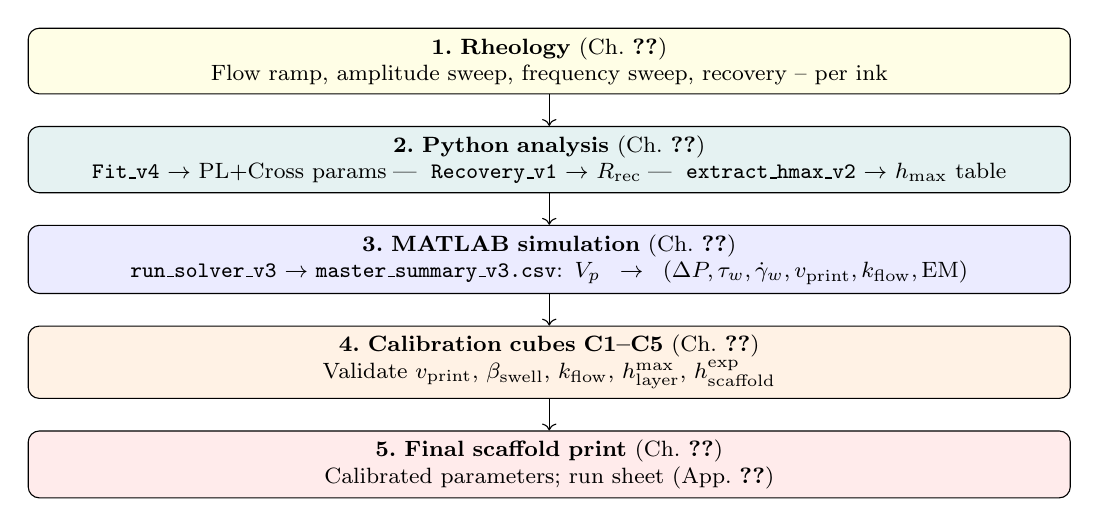
\begin{tikzpicture}[node distance=4mm,
    every node/.style={font=\footnotesize, align=center}]
  \node[draw, rounded corners, fill=yellow!10, text width=13cm]
    (rheo) {\textbf{1.~Rheology} (Ch.~\ref{sec:tests})\\
    Flow ramp, amplitude sweep, frequency sweep, recovery -- per ink};
  \node[draw, rounded corners, fill=teal!10, text width=13cm, below=of rheo]
    (py) {\textbf{2.~Python analysis} (Ch.~\ref{sec:python})\\
    \texttt{Fit\_v4} $\to$ PL+Cross params\;|\;
    \texttt{Recovery\_v1} $\to$ $R_\mathrm{rec}$\;|\;
    \texttt{extract\_hmax\_v2} $\to$ $h_\mathrm{max}$ table};
  \node[draw, rounded corners, fill=blue!8, text width=13cm, below=of py]
    (mat) {\textbf{3.~MATLAB simulation} (Ch.~\ref{sec:matlab})\\
    \texttt{run\_solver\_v3} $\to$ \texttt{master\_summary\_v3.csv}:
    $V_p\to(\Delta P,\tau_w,\gd_w,v_\mathrm{print},k_\mathrm{flow},\mathrm{EM})$};
  \node[draw, rounded corners, fill=orange!10, text width=13cm, below=of mat]
    (cube) {\textbf{4.~Calibration cubes C1--C5} (Ch.~\ref{sec:cubes})\\
    Validate $v_\mathrm{print}$, $\beta_\mathrm{swell}$, $k_\mathrm{flow}$,
    $h_\mathrm{layer}^{\max}$, $h_\mathrm{scaffold}^\mathrm{exp}$};
  \node[draw, rounded corners, fill=red!8, text width=13cm, below=of cube]
    (final) {\textbf{5.~Final scaffold print} (Ch.~\ref{sec:final})\\
    Calibrated parameters; run sheet (App.~\ref{app:runsheet})};
  \draw[->] (rheo)--(py); \draw[->] (py)--(mat);
  \draw[->] (mat)--(cube); \draw[->] (cube)--(final);
\end{tikzpicture}

\medskip The next sections describe steps 2--5 in operational detail.
For step 1, see Ch.~\ref{sec:tests}; for the theoretical rationale
of each output, see Part~I.

% -----------------------------------------------------------------
\section{Step 2: Python Analysis}
\label{sec:python}

\subsection{Pre-run checklist}
\begin{itemize}[leftmargin=1.4em,itemsep=1pt]
\item[$\square$] Activate the project Python environment.
\item[$\square$] Verify \texttt{xlrd}, \texttt{scipy}, \texttt{numpy},
  \texttt{pandas}, and \texttt{matplotlib} are installed.
\item[$\square$] Check that the \texttt{.xls} files from the Anton Paar
  are in the expected folders (\texttt{Reologia/Viscosity/},
  \texttt{Reologia/Strain/}, \texttt{Reologia/Frequency/},
  \texttt{Reologia/Recovery/}).
\item[$\square$] Confirm the active script is
  \texttt{Fit\_Muitos\_Modelos\_v4.py} (see CLAUDE.md \S6.9).
\end{itemize}

\subsection{Flow-curve fitting -- \texttt{Fit\_Muitos\_Modelos\_v4.py}}

\begin{lstlisting}[style=shell]
cd Analises/Python
python3 Fit_Muitos_Modelos_v4.py
# Outputs: Results/FitAll-Ramp1-v4.txt
#          Results/FitAll-Ramp2-v4.txt  (if Flow Sheared run)
# Contains: PL (K, n) and Cross (eta_0, eta_inf, lambda, m)
#           with R^2, AIC, BIC per model per ink.
\end{lstlisting}

\paragraph{What to check.}
\begin{itemize}[leftmargin=1.4em,itemsep=1pt]
\item $R^2\geq 0.98$ for Cross across the full $\gd$ range.
\item Cross $\eta_\infty$ is finite and positive (not pinned to its
  lower bound -- check that AIC/BIC improved over a 3-parameter fit).
\item Cross AIC/BIC lower than PL on log-spaced data.
\item PL parameters agree with the Cross slope in the printable
  $\gd_w$ range (50--1000\,\si{\per\s}).
\item If $R^2<0.95$ for Cross: suspect multi-mode behaviour or a
  data quality issue (bubble, edge effects); flag before proceeding.
\end{itemize}

\subsection{Recovery -- \texttt{Recovery\_v1.py}}

\begin{lstlisting}[style=shell]
python3 Recovery_v1.py
# Output: Results/Relatorio_Recovery.txt
# Reports R_rec(%) at t=30s for each (ink, gamma_dot_2).
\end{lstlisting}

\paragraph{What to check.}
$R_\mathrm{rec}$ should decrease monotonically (or remain flat) with
increasing $\gd_2$. A non-monotonic pattern (e.g.\ higher recovery at
100 than at 50\,\si{\per\s}) typically means the recovery test was
contaminated by the preceding amplitude sweep (network not fully rebuilt).
Repeat with a fresh sample; wait $\geq 5\,\si{\minute}$ between tests.

\subsection{Scaffold-height extraction -- \texttt{extract\_hmax\_v2.py}}

\begin{lstlisting}[style=shell]
python3 extract_hmax_v2.py
# Outputs:
#   Results/SAOS_hmax_v2.txt
#   Results/printing_parameters_per_ink.csv
#   Results/Gprime_extrap_<ink>.png
# Reports h_scaffold_max under criteria A, B, C and N_max.
\end{lstlisting}

\paragraph{What to check.}
The $G'(\omega)$ log-log plot (\texttt{Gprime\_extrap\_<ink>.png})
should be visually linear at the low-$\omega$ end. If the lowest-frequency
points scatter, trim the fit window upward by one point and re-run;
the low-$\omega$ extrapolation is sensitive to noise.

% -----------------------------------------------------------------
\section{Step 3: MATLAB Simulation -- \texttt{run\_solver\_v3.m}}
\label{sec:matlab}

\begin{lstlisting}[style=shell]
cd Analises/MatLab
matlab -batch "run_solver_v3"
# Loops: 3 inks x 2 needles (21G, 22G) x 8 piston velocities.
# Outputs:
#   output_v3/slicer_lookup_<ink>_<needle>.csv
#   output_v3/plots_<ink>_<needle>.png  (4-panel summary)
#   output_v3/master_summary_v3.csv     (reference row Vp=0.01)
\end{lstlisting}

\paragraph{Reading \texttt{master\_summary\_v3.csv}.}
Columns (in order): sample, needle, $V_p$ | $v_\mathrm{print}$ (PL and
Cross) | $\Delta P$ | $\tau_w$ | $\gd_w$ | $w_\mathrm{line}$ |
$h_\mathrm{layer}$ | $k_\mathrm{flow}$ | $\mathrm{EM}_\mathrm{slicer}$.

\begin{warningbox}
The CSV column is $k_\mathrm{flow}$, \emph{not}
$\mathrm{EM}_\mathrm{slicer}$. Read the $\mathrm{EM}_\mathrm{slicer}$
column (the last column in the lookup CSV, added in v3) for the number
to type into the slicer. If you use an older CSV, compute
$\mathrm{EM}=1/k_\mathrm{flow}$ by hand. Never type $k_\mathrm{flow}$
directly into the slicer.
\end{warningbox}

\begin{tipbox}
The default reference row is at $V_p=0.01\,\mms$. For a different
operating point, open the per-ink CSV
\texttt{slicer\_lookup\_<ink>\_<needle>.csv} which covers the full
$V_p\in\{0.003\ldots 0.04\}\,\mms$ sweep.
\end{tipbox}

\paragraph{When to re-run the MATLAB simulation.}
Any time Python produces new Cross or Power-Law parameters, update
the \texttt{samples} struct in \texttt{run\_solver\_v3.m} and re-run.
Parameters must always be in sync between Python output and MATLAB input.

% -----------------------------------------------------------------
\section{Step 4: Calibration-Cube Protocol (C1--C5)}
\label{sec:cubes}

\textbf{Run all tests on the same day, with the same syringe load.}
Each test is a diagnostic for one physical question; if it fails, the
failure mode points to one rheological input.

\paragraph{Pre-calibration checklist.}
\begin{itemize}[leftmargin=1.4em,itemsep=1pt]
\item[$\square$] Power up printer, home all axes, level bed.
\item[$\square$] Pull ink from $4\,^\circ$C storage; let it equilibrate
  at $25\,^\circ$C for $\geq 30\,\si{\minute}$.
\item[$\square$] Re-homogenise by slow inversion (30 times); inspect for
  phase separation or air bubbles.
\item[$\square$] Load syringe; mount needle; prime until steady bead exits.
\item[$\square$] Enter $V_p$, $\mathrm{EM}_\mathrm{slicer}$, and
  $h_\mathrm{layer}$ from the lookup CSV into the slicer.
\item[$\square$] Verify predicted $\Delta P<1500\,\si{\kPa}$ from CSV.
\end{itemize}

\subsection{C1 -- print-speed sweep}

\begin{stepbox}{C1: identify the optimum $v_\mathrm{print}$ at fixed $V_p$}
Print five $30\,\si{\mm}$ straight filaments on a clean glass slide at
five XY feedrates $v_\mathrm{print}\in\{5,10,20,30,50\}\,\mms$, keeping
$V_p$ fixed at the lookup-CSV value. Wait 5\,\si{\minute}. Under a
microscope, measure filament width $d_\mathrm{fil}$ at three points per
filament.

\textbf{Optimum:} the $v_\mathrm{print}$ at which
$0.95\leq d_\mathrm{fil}/\mathrm{ID}\leq 1.10$.
Below 0.95: head outruns ink supply (under-extrusion or motor skip).
Above 1.10: over-deposition or accumulated die swell.

\textbf{Also read die swell:} measure $w_\mathrm{line}$ at the optimum
$v_\mathrm{print}$; compute $\beta_\mathrm{swell}^\mathrm{exp}=
w_\mathrm{line}/\mathrm{ID}-1$ and compare against the proxy from the
lookup CSV. Update if $|\beta^\mathrm{exp}-\beta^\mathrm{pred}|>0.05$.
\end{stepbox}

\subsection{C2 -- mass-per-line ($k_\mathrm{flow}$) calibration}

\begin{stepbox}{C2: measure $k_\mathrm{flow}^\mathrm{exp}$ and update $\mathrm{EM}$}
At the C1-optimum $v_\mathrm{print}$, print ten parallel $30\,\si{\mm}$
lines on a tared glass slide with $1\,\si{\mm}$ spacing. Time the print.
Reweigh; convert to volume using $\rho_\mathrm{ink}=1.00\,\si{\g/cm^3}$.
\[
k_\mathrm{flow}^\mathrm{exp}
=\frac{V_\mathrm{measured}}{v_\mathrm{print}\cdot w_\mathrm{line}\cdot
h_\mathrm{layer}\cdot t_\mathrm{print}}.
\]
\textbf{Invert and enter}
$\mathrm{EM}^\mathrm{exp}=1/k_\mathrm{flow}^\mathrm{exp}$ as the slicer's
Extrusion Multiplier for all subsequent prints with this ink and needle.
\end{stepbox}

\subsection{C3 -- layer-height sweep}

\begin{stepbox}{C3: find $h_\mathrm{layer}^{\max}$}
Print a 3-layer $10\times 10\,\si{\mm}$ square at three layer heights
$h_\mathrm{layer}\in\{0.30,0.40,0.50\}\,\si{\mm}$. After
30\,\si{\minute} of relaxation, measure the total stack height.

$h_\mathrm{layer}^{\max}$: the largest $h_\mathrm{layer}$ at which
measured total height $\geq 90\%$ of commanded total $3h_\mathrm{layer}$.
\end{stepbox}

\subsection{C4 -- vertical-tower test}

\begin{stepbox}{C4: validate $h_\mathrm{scaffold}^{\max}$ from SAOS}
Print a $5\times 5\,\si{\mm}$ tower at $h_\mathrm{layer}^{\max}$ from
C3, up to $N=40$ layers (or the predicted $N_\mathrm{max}$ from
\texttt{printing\_parameters\_per\_ink.csv}, whichever is smaller).
Photograph every 5 layers and at $t=30\,\si{\minute}$.

$h_\mathrm{scaffold}^\mathrm{exp}$: height at which base width grows
by $>10\%$. Record which SAOS criterion best matches the collapse onset.
\textbf{Use that criterion for all future prints of this ink at similar
dwell times.}
\end{stepbox}

\subsection{C5 (optional) -- bridging test for lattice scaffolds}

\begin{stepbox}{C5: unsupported-span sag test}
Print three pairs of $20\,\si{\mm}$ pillars at gap lengths
$L\in\{0.5,1.0,2.0\}\,\si{\mm}$. Print a single bridging filament over
each gap; measure mid-span sag after 5\,\si{\minute}. Compare against
Smay prediction (Eq.~\ref{eq:smay}). If sag exceeds the prediction, the
strut span must be shortened.
\end{stepbox}

\begin{runningbox}{RUNNING EXAMPLE -- Solution to Q6}
\textbf{Question.} What does Ana's Wednesday morning look like?

\medskip\textbf{Schedule ($\sim 4$--$5\,\si{\hour}$):}

\medskip
\begin{tabular}{p{2.0cm} p{12.5cm}}
\toprule
\textsl{08:30} & Power up; home; level. Pull C15 Gira~5.5 from $4\,^\circ$C;
equilibrate 30\,\si{\minute}. \\
\textsl{09:00} & Re-homogenise; load syringe; prime. Enter $V_p=0.01\,\mms$,
$\mathrm{EM}=1.49$, $h_\mathrm{layer}=0.36\,\si{\mm}$ in slicer.
Predicted $\Delta P=164\,\si{\kPa}$: proceed. \\
\textsl{09:30} & \textbf{C1.} Five filaments at $v_\mathrm{print}\in
\{5,10,20,30,50\}\,\mms$. Microscope. Expected optimum near $10\,\mms$. \\
\textsl{10:30} & \textbf{C2.} Ten lines on tared slide; weigh.
Expected $k_\mathrm{flow}^\mathrm{exp}\in[0.6,0.8]$;
$\mathrm{EM}^\mathrm{exp}\in[1.25,1.67]$. \\
\textsl{11:30} & \textbf{C3.} Three 3-layer squares at
$h_\mathrm{layer}\in\{0.30,0.40,0.50\}\,\si{\mm}$. Wait 30\,\si{\minute}.
Expected $h_\mathrm{layer}^{\max}\approx 0.40\,\si{\mm}$. \\
\textsl{13:00} & \textbf{C4.} Tower at $h_\mathrm{layer}^{\max}$;
target $N=56$ ($=20\,\si{\mm}$). Stop early if base bulges. \\
\textsl{15:00} & Done. Log all calibrated parameters to
\texttt{lab\_calibration\_log.csv}. \\
\bottomrule
\end{tabular}

\medskip\textbf{Go / No-go.} If calibrated parameters match predictions
within 30\% and C4 tower clears $\sim 50$ layers cleanly: proceed to
Thursday production print. Otherwise: escalate before burning more ink.
\end{runningbox}

% -----------------------------------------------------------------
\section{Step 5: Final Scaffold Print}
\label{sec:final}

After C1--C4, the slicer profile contains all five validated entries:
\begin{itemize}[leftmargin=1.4em,itemsep=2pt]
\item $V_p$ (E-axis feedrate) at the validated value.
\item $v_\mathrm{print}$ (XY feedrate) at the C1 optimum.
\item $\mathrm{EM}^\mathrm{exp}=1/k_\mathrm{flow}^\mathrm{exp}$ from C2.
\item $h_\mathrm{layer}\leq h_\mathrm{layer}^{\max}$ from C3.
\item Total scaffold height $\leq h_\mathrm{scaffold}^\mathrm{exp}$ from C4.
\end{itemize}

Save slicer profile as \texttt{<ink>\_<needle>\_<scaffold>\_v<n>.ini}.
Record the final print on the run sheet (App.~\ref{app:runsheet}).

% -----------------------------------------------------------------
\section{Troubleshooting: Failure-Mode Decision Tree}
\label{sec:troubleshoot}

\begin{table}[h]
\centering\small
\begin{tabular}{p{3.5cm} p{3.5cm} p{6.0cm}}
\toprule
\textbf{Observation} & \textbf{Physical root cause} & \textbf{Action} \\
\midrule
Motor hum / skip; no flow &
  $\Delta P$ exceeds motor stall, or clog &
  Lower $V_p$ 25\%. If still no flow: switch to wider needle; purge. \\
$d_\mathrm{fil}/\mathrm{ID}>1.2$ consistently &
  Over-extrusion or $\beta_\mathrm{swell}$ underestimated &
  Lower $\mathrm{EM}$ in 0.05 steps; measure $\beta^\mathrm{exp}$ in C1. \\
$d_\mathrm{fil}/\mathrm{ID}<0.9$ consistently &
  Under-extrusion or motor skip &
  Raise $\mathrm{EM}$ in 0.05 steps; verify $\Delta P$ vs.\ motor limit. \\
Tower base bulges at low $N$ &
  $\sigma_\mathrm{stack}$ exceeded at effective timescale &
  Reduce target height; increase $v_\mathrm{print}$; switch ink. \\
Tower buckles sideways &
  Smay lattice buckling &
  Shorten span or use higher-$G'$ ink. \\
Layer fusion / mushy scaffold &
  $h_\mathrm{layer}>h_\mathrm{layer}^{\max}$ or low $R_\mathrm{rec}$ &
  Decrease $h_\mathrm{layer}$; increase $v_\mathrm{travel}$. \\
Stringing on travel moves &
  Slow recovery at travel timescale &
  Set retraction to \textbf{zero}; increase $v_\mathrm{travel}$. \\
Rough filament surface &
  Elastic extrudate instability &
  Lower $V_p$; use longer needle. \\
First-layer adhesion failure &
  Bed clean / Z-zero / temperature &
  Clean bed; raise first-layer $h$ by 0.05\,\si{\mm}; re-home. \\
\bottomrule
\end{tabular}
\caption{Operator troubleshooting decision tree. All corrective actions
target $V_p$, $\mathrm{EM}$, geometry, or needle gauge. $\Delta P$
is an output and is never adjusted directly.}
\label{tab:troubleshoot}
\end{table}

% -----------------------------------------------------------------
\section{The Friday Print -- Closing the Loop}
\label{sec:friday}

By Wednesday 15:00, Ana has answered every question this book posed:
\begin{itemize}[leftmargin=1.4em,itemsep=2pt]
\item \textbf{Q1.} The ink is a reinforced critical gel with wide LVR --
  excellent DIW candidate.
\item \textbf{Q2.} $V_p=0.01\,\mms$ to reach $v_\mathrm{print}\approx
  8\,\mms$.
\item \textbf{Q3.} $\Delta P\approx 164\,\si{\kPa}$ -- safe.
  $\tau_w=663\,\si{\Pa}$ -- cell-safe.
\item \textbf{Q4.} $k_\mathrm{flow}\approx 0.67$;
  $\mathrm{EM}=1.49$ into the slicer.
\item \textbf{Q5.} 20-mm block feasible under criterion B; validated by C4.
\item \textbf{Q6.} Calibration completed 08:30--15:00; no surprises.
\end{itemize}

\textbf{Thursday, 10:00.} Ana exports G-code, mounts a fresh syringe of
conditioned ink, and prints the $1\times 1\times 2$\,cm$^3$ block.
Total print time $\approx 45\,\si{\minute}$. The block holds its shape.
She photographs at $t=0$, $t=30\,\si{\minute}$, and $t=24\,\si{\hour}$.

\textbf{Friday, 15:30.} Ana hands the supervisor the scaffold and the
completed run sheet.

\medskip\textbf{The pedagogical point.} Every entry on Ana's run sheet
was computed from a rheological measurement and one equation chain. The
slicer firmware was treated as a dumb FFF tool that needed translation.
The rheometer told her what the ink wanted; the math told her what to
type; the calibration cubes told her where the math was off and by how
much. \emph{This is the framework. The rest is execution.}

\bigskip\hrule\bigskip

% =================================================================
% PART IV -- EXTENDED TOPICS
% =================================================================
\part*{Part IV -- Extended Topics}
\addcontentsline{toc}{part}{Part IV -- Extended Topics}

% =================================================================
\section{Biological and Regulatory Considerations}
\label{sec:bio}

\subsection{Cell viability and wall shear stress}

\emph{Motivation.} Cells fail at the wall, not at the average shear: the parabolic (or
near-parabolic) velocity profile concentrates stress in the thin annular
layer closest to the needle surface, while the central core experiences
far lower shear.  Moreover, damage is a cumulative dose, not just a
peak: a modest $\tau_w$ sustained over a long needle transit can cause as
much membrane fatigue as a brief, high-stress spike.

The primary mechanical threat to cells during DIW extrusion is the wall
shear stress $\tau_w$. Literature consensus \citep{BlaeserEtAl2016}
places the acute viability threshold at:
\begin{equation}
\tau_w^\mathrm{safe} \;\lesssim\; 5\,\si{\kPa}.
\label{eq:tauw_safe}
\end{equation}
Above this threshold, cell membrane rupture and cytoskeletal damage
increase sharply. For the inks in this project, $\tau_w$ at the nominal
$V_p$ is 460--660\,\si{\Pa} -- one order of magnitude below the threshold.
This provides substantial margin for cell-loaded future prints.

\begin{derivationbox}[title={DERIVATION --- Cumulative shear dose $D_\mathrm{shear}$}]
\textbf{Goal.} Quantify the total mechanical dose experienced by a cell
transiting the needle once.

\medskip
\textbf{Residence time.}
A cell entering the needle at the syringe--needle junction exits at the
tip after travelling the full needle length $L_n$.  Using the mean needle
velocity $\bar v_n = (R_s/R_n)^2\,V_p$ (Eq.~\ref{eq:vbar_n}), the
transit time is:
\begin{equation}
t_\mathrm{res} \;=\; \frac{L_n}{\bar v_n}
               \;=\; \frac{L_n}{\,(R_s/R_n)^2\,V_p\,}.
\label{eq:t_res}
\end{equation}
For the 21G needle used in this project
($L_n=\SI{31.75}{\mm}$, $(R_s/R_n)^2=771$) at
$V_p=\SI{0.01}{\mm\per\s}$:
\[
t_\mathrm{res} \;=\; \frac{31.75}{771\times 0.01}
               \;=\; \frac{31.75}{7.71}
               \;\approx\; \SI{4.12}{\s}.
\]

\medskip
\textbf{Cumulative shear dose.}
The shear stress field $\tau(r)$ peaks at the wall ($r=R_n$) and
decreases toward the centreline.  As a conservative bound, every cell
is exposed to $\tau_w$ throughout the transit (this overestimates
damage for cells in the core, but is the safe design choice).  The
cumulative dose is then:
\begin{equation}
D_\mathrm{shear}
  \;=\; \int_0^{t_\mathrm{res}} \tau(t)\,dt
  \;\approx\; \tau_w\,t_\mathrm{res}
  \qquad [\si{\Pa\s}].
\label{eq:shear_dose}
\end{equation}

\medskip
\textbf{Why both criteria matter.}
A wide-gauge, short needle may satisfy $\tau_w<\SI{5}{\kPa}$ yet still
deliver a damaging $D_\mathrm{shear}$ if the syringe-to-needle area ratio
is small (low $\bar v_n$, long $t_\mathrm{res}$).  Conversely, a very
fine needle at high $V_p$ may have a large $\tau_w$ but negligible dose
because $t_\mathrm{res}$ is extremely short.  Both limits must be
checked: peak $\tau_w<\SI{5}{\kPa}$ \textit{and}
$D_\mathrm{shear}=\tau_w\,t_\mathrm{res}$ below the cell-type tolerance.
\end{derivationbox}

\paragraph{Cell type sensitivity.}
Different cell lines have different shear thresholds:
\begin{itemize}[leftmargin=1.4em,itemsep=2pt]
\item Osteoblasts and fibroblasts: relatively resistant; tolerate
  $\tau_w\leq 10\,\si{\kPa}$ for brief exposures.
\item Stem cells (MSC, iPSC): more sensitive; threshold closer to
  5\,\si{\kPa}.
\item Chondrocytes: sensitive to both shear and compression history.
\end{itemize}
For any cell type, measure post-print viability (live/dead assay within
2\,\si{\hour} of printing) and compare against unprinted controls. Do
not assume compliance from literature thresholds alone.

\subsection{Plug flow and cell protection}

The radial stress profile $\tau(r)=\tau_w(r/R_n)$ vanishes at the
centreline and rises to $\tau_w$ at the wall.  For a yield-stress ink,
the central region where $\tau<\tau_y$ is never sheared at all -- it
translates as a solid plug, and any cell inside it experiences
\textit{zero} shear stress during transit.  Understanding the size of
this plug is therefore the single most important geometric quantity for
cell-viability engineering.

\begin{derivationbox}[title={DERIVATION --- Plug radius and shear-free cell fraction}]
\textbf{Stress profile.}
For fully developed flow in a tube of radius $R_n$ and length $L_n$,
the axial pressure gradient $\Delta P/L_n$ drives flow and the local
shear stress varies linearly with radius:
\begin{equation}
\tau(r) \;=\; \frac{\Delta P}{2L_n}\,r \;=\; \tau_w\,\frac{r}{R_n}.
\label{eq:tau_profile}
\end{equation}
At $r=R_n$ this gives $\tau_w=\Delta P\,R_n/(2L_n)$, confirming the
wall stress formula used throughout Ch.~\ref{sec:hydraulic_loop}.

\medskip
\textbf{Plug radius.}
The unyielded (plug) core exists wherever $\tau(r)\leq\tau_y$:
\begin{equation}
\tau_w\,\frac{r_0}{R_n} \;=\; \tau_y
\quad\Longrightarrow\quad
\frac{r_0}{R_n} \;=\; \frac{\tau_y}{\tau_w}.
\label{eq:r0_over_R}
\end{equation}
Substituting $\tau_w = \Delta P\,R_n/(2L_n)$:
\[
r_0 \;=\; R_n\,\frac{\tau_y}{\tau_w}
     \;=\; R_n\cdot\frac{2L_n\tau_y}{\Delta P\,R_n}
     \;=\; \frac{2L_n\,\tau_y}{\Delta P},
\]
which is the standard Bingham result: the plug radius grows with yield
stress and needle length and shrinks with applied pressure.

\medskip
\textbf{Shear-free cell fraction.}
Cells are uniformly distributed across the cross-section (area
$\pi R_n^2$).  The protected (plug) area is $\pi r_0^2$.  Therefore the
fraction of cells that experience \emph{zero} shear during transit is:
\begin{equation}
f_\mathrm{core}
  \;=\; \left(\frac{r_0}{R_n}\right)^{\!2}
  \;=\; \left(\frac{\tau_y}{\tau_w}\right)^{\!2}.
\label{eq:f_core}
\end{equation}
Conversely, the fraction exposed to high shear is
$f_\mathrm{wall}=1-f_\mathrm{core}=1-(\tau_y/\tau_w)^2$.

\medskip
\textbf{Consistency with the Bingham number.}
From the definition $\Bi=\tau_y/(\eta_p\,\gd_w)$ and the Bingham
constitutive law $\tau_w=\tau_y+\eta_p\,\gd_w$, one obtains:
\[
\frac{\tau_y}{\tau_w}
  \;=\; \frac{\tau_y}{\tau_y+\eta_p\,\gd_w}
  \;=\; \frac{1}{1+\eta_p\,\gd_w/\tau_y}
  \;=\; \frac{\Bi}{\Bi+1}.
\]
Substituting into Eq.~\ref{eq:r0_over_R}:
\begin{equation}
\frac{r_0}{R_n} \;=\; \frac{\Bi}{\Bi+1}.
\label{eq:r0_Bi}
\end{equation}
This is exactly the expression derived in the Hydraulic-Loop
plug-flow exercise (Ch.~\ref{sec:hydraulic_loop}).
As $\Bi\to\infty$, $r_0/R_n\to 1$: the entire cross-section
translates as a rigid plug and virtually all cells are shear-free.
As $\Bi\to 0$ (Newtonian limit), $r_0\to 0$ and all cells experience
the full parabolic shear field.
\end{derivationbox}

\begin{inpracticebox}[title={IN PRACTICE --- Designing for cell viability in DIW}]
\begin{itemize}[leftmargin=1.4em,itemsep=3pt]
\item \textbf{Choose the widest needle the resolution allows.}
  Switching from 22G to 21G at fixed $V_p$ reduces $\tau_w$ by
  roughly half (recall $\tau_w\propto R_n^{-(3+n)}$ with $n<1$) and
  increases $t_\mathrm{res}$ only modestly, giving a net reduction in
  both peak stress and dose.
\item \textbf{Use the lowest $V_p$ that clears the minimum dwell time.}
  Lowering $V_p$ reduces $\bar v_n=(R_s/R_n)^2 V_p$, which lowers
  $\gd_w$ and $\tau_w$. The penalty is a longer $t_\mathrm{res}$, but
  for shear-thinning inks the $\tau_w$ reduction dominates, so the dose
  $D_\mathrm{shear}=\tau_w\,t_\mathrm{res}$ typically falls.
\item \textbf{Maximise the Bingham number.}
  Formulate inks with as high a yield stress as possible while
  maintaining $\tau_w<\SI{5}{\kPa}$: a large $\Bi$ means a large
  $r_0/R_n=\Bi/(\Bi+1)$ and most cells ride the shear-free plug.
\item \textbf{Compute $D_\mathrm{shear}$ before printing.}
  Use Eq.~\ref{eq:shear_dose}: $D_\mathrm{shear}=\tau_w\,L_n/\bar v_n$.
  For multi-layer prints each cell passes the needle once, so cumulative
  dose equals $D_\mathrm{shear}$ per layer multiplied by the number of
  times that cell is re-extruded (usually once for scaffold prints).
\end{itemize}
\end{inpracticebox}

\begin{takeawaybox}
\begin{itemize}[leftmargin=1.4em,itemsep=2pt]
\item Peak wall stress $\tau_w<\SI{5}{\kPa}$ is necessary but not
  sufficient for cell safety; the cumulative dose
  $D_\mathrm{shear}=\tau_w\,t_\mathrm{res}$ must also be checked.
\item A high Bingham number ($\Bi\gg1$) creates a large shear-free plug:
  $f_\mathrm{core}=(\Bi/(\Bi+1))^2\to1$.  This is the principal
  rheological lever for protecting cells in DIW.
\item For the project inks at $V_p=\SI{0.01}{\mm\per\s}$ on a 21G needle,
  $\tau_w\approx\SI{663}{\Pa}$ and $D_\mathrm{shear}\approx\SI{2.7}{\kPa\s}$
  -- well inside acute safety margins, providing a comfortable baseline for
  future cell-loading studies.
\end{itemize}
\end{takeawaybox}

\begin{exercise}{\diffB}
\textbf{Cumulative shear dose.}
A 21G needle ($R_n=\SI{0.2575}{\mm}$, $L_n=\SI{31.75}{\mm}$) is used
with $V_p=\SI{0.01}{\mm\per\s}$.  The syringe-to-needle area ratio is
$(R_s/R_n)^2=771$ (standard 10\,mL BD syringe).
\begin{enumerate}[label=(\alph*),leftmargin=1.6em,itemsep=1pt]
  \item Compute the mean needle velocity $\bar v_n$.
  \item Compute the needle residence time $t_\mathrm{res}$.
  \item The NE ink has wall shear stress $\tau_w=\SI{663}{\Pa}$ at this
    operating point.  Compute the cumulative shear dose
    $D_\mathrm{shear}=\tau_w\,t_\mathrm{res}$ in \si{\Pa\s}.
  \item Is $\tau_w$ within the acute viability threshold (Eq.~\ref{eq:tauw_safe})?
    Comment on whether $D_\mathrm{shear}$ raises additional concerns.
\end{enumerate}
\begin{solution}
(a) $\bar v_n = 771\times 0.01 = \SI{7.71}{\mm\per\s}$.

(b) $t_\mathrm{res} = L_n/\bar v_n = 31.75/7.71 \approx \SI{4.12}{\s}$.

(c) $D_\mathrm{shear} = 663\times 4.12 \approx \SI{2732}{\Pa\s}
    \approx \SI{2.7}{\kPa\s}$.

(d) Yes: $\tau_w = \SI{663}{\Pa} \ll \SI{5}{\kPa}$, so the acute peak
criterion is comfortably satisfied (factor $\sim$7.5 of safety margin).
The dose $D_\mathrm{shear}\approx\SI{2.7}{\kPa\s}$ is moderate; for
most adherent cell types this single-transit dose is acceptable, but it
should be recorded and compared against cell-type-specific tolerance
values. Multi-pass prints (if any cell traverses the needle more than
once) would multiply this figure and require re-evaluation.
\end{solution}
\end{exercise}

\begin{exercise}{\diffC}
\textbf{Plug-core fraction and the Bingham number.}
A cell-loaded Bingham ink with $\Bi=12$ is extruded through a 21G needle
($R_n=\SI{0.2575}{\mm}$) at the nominal print speed.
\begin{enumerate}[label=(\alph*),leftmargin=1.6em,itemsep=1pt]
  \item Using $r_0/R_n=\Bi/(\Bi+1)$ (Eq.~\ref{eq:r0_Bi}), compute the
    plug radius as a fraction of $R_n$.
  \item What fraction of the needle cross-sectional area is occupied by
    the shear-free plug?
  \item If the same formulation is extruded through a 22G needle at the
    same $V_p$, qualitatively does $\Bi$ increase or decrease?  Is the
    change beneficial for cell viability?
\end{enumerate}
\begin{solution}
(a) $r_0/R_n = 12/(12+1) = 12/13 \approx 0.923$.

(b) $f_\mathrm{core} = (r_0/R_n)^2 = (12/13)^2 = 144/169
    \approx 0.852$, i.e.\ approximately \textbf{85\%} of the
    cross-sectional area is shear-free.  Only the outermost 15\% of the
    area (a thin annulus of thickness $\approx0.077\,R_n\approx
    \SI{20}{\micro\m}$) experiences wall-level shear stress.

(c) Switching to 22G at fixed $V_p$: $R_n$ decreases
($0.2575\to\SI{0.2065}{\mm}$), so $\gd_w\propto R_n^{-3}$ rises
and $\tau_w\propto R_n^{-(3+n)}$ rises faster; $\tau_y$ is a material
property and does not change.  Therefore
$\Bi=\tau_y/(\eta_p\gd_w)$ \emph{decreases}: the plug shrinks.
The change is \textbf{detrimental} -- a smaller $f_\mathrm{core}$
means more cells are exposed to the higher (and now larger) $\tau_w$.
For cell-loaded prints, the widest needle meeting the resolution
requirement minimises damage.
\end{solution}
\end{exercise}

\subsection{Long-duration print considerations}

For prints lasting $>30\,\si{\minute}$ with cell-loaded inks:
\begin{itemize}[leftmargin=1.6em,itemsep=2pt]
\item Keep the unused ink at $4\,^\circ$C or on ice; avoid temperature
  fluctuations that change rheology mid-print.
\item Monitor filament width at intervals (every 10 layers); drift
  indicates ink dewatering or temperature change.
\item Consider enclosing the printer in a humidified chamber to prevent
  evaporation from the deposited scaffold.
\end{itemize}

\subsection{MAPA-oriented regulatory considerations}

For healthcare applications in Brazil (pharmaceutical or dermocosmetic
products), the National Health Surveillance Agency (ANVISA) and the
Ministry of Agriculture, Livestock, and Food Supply (MAPA) impose
requirements on the production process:

\begin{itemize}[leftmargin=1.6em,itemsep=2pt]
\item \textbf{Raw material traceability.} The CMC grade, molecular weight
  determination method (cite \citealt{daSilva2018}), and NE formulation
  parameters (oil type, surfactant, batch number) must all be documented.
\item \textbf{Process reproducibility.} Calibration data (C1--C4 outputs)
  must be recorded and archived per batch.
\item \textbf{Biocompatibility testing.} For dermocosmetic applications
  (e.g.\ Amphotericin B carrier), ISO 10993-5 cytotoxicity testing is
  required. The current project phase is pre-regulatory (acellular
  scaffold characterisation only).
\item \textbf{Scale-up validation.} The DIW parameters characterised on
  the lab-scale piston printer must be re-validated at pilot scale;
  scale-up introduces pressure gradients and syringe-wall effects not
  present at 10\,mL scale.
\end{itemize}

\begin{tipbox}
When writing the manuscript, frame the DIW as a ``proof-of-concept
fabrication platform'' rather than a production process. This framing
keeps the paper in the research domain and defers the regulatory
validation discussion to future work.
\end{tipbox}

% =================================================================
\section{Statistical Optimisation: DOE and Response Surface Methodology}
\label{sec:doe}

\subsection{Overview}

Design of Experiments (DOE) and Response Surface Methodology (RSM)
are the standard tools for optimising the NE formulation (oil fraction,
surfactant type, surfactant concentration, homogenisation protocol)
with respect to measured responses (droplet size, $\eta_0$, $G'_\mathrm{LVR}$,
printability). This section documents the critical decisions required
before running any RSM, with emphasis on categorical variables -- the
most common source of invalid models in this type of study.

\subsection{Continuous vs.\ categorical variables}

RSM models assume all factors are \emph{continuous}: they can take any
value in a range, and the response varies smoothly with them. A factor
is \emph{categorical} if it takes discrete, unordered levels with no
implied metric distance between them.

\textbf{Continuous factors} (safe for RSM quadratic terms):
\begin{itemize}[leftmargin=1.4em,itemsep=1pt]
\item Oil mass fraction [\%]
\item Surfactant concentration [mg/mL]
\item Homogenisation speed [rpm]
\item Homogenisation time [min]
\end{itemize}

\textbf{Categorical factors} (cannot receive quadratic terms in RSM):
\begin{itemize}[leftmargin=1.4em,itemsep=1pt]
\item Surfactant type (Tween 80 / Span 80 / Polysorbate 20 / \ldots)
\item Emulsification method (probe sonication / high-pressure HPH /
  rotor-stator)
\item Needle type (blunt / tapered)
\item Pulse mode (on/off), if coded as 1/0
\end{itemize}

\begin{warningbox}
\textbf{Categorical variables must not appear in quadratic RSM terms.}
A quadratic term for ``surfactant type'' (e.g.\ $x_\mathrm{surfactant}^2$
where surfactant type is coded as 1, 2, 3) imposes an implied quadratic
distance between surfactant types that has no physical meaning. The
resulting ``optimal'' surfactant is often a non-existent interpolation
between two real options.

\medskip\textbf{Correct handling:} Run separate RSM surfaces for each
level of the categorical factor, or use mixture designs, or test only
one categorical level at a time with a fixed level for all others.
\end{warningbox}

\subsection{Model selection recommendations}

\begin{itemize}[leftmargin=1.6em,itemsep=3pt]
\item For 2--4 continuous factors: full Central Composite Design (CCD)
  or Box-Behnken Design. Minimum 5 centre-point replicates for pure
  error estimation.
\item For $>4$ continuous factors: use a D-optimal or I-optimal custom
  design to keep run count manageable.
\item For one categorical factor: use a split-plot design or run separate
  CCD blocks per categorical level.
\item Always report the lack-of-fit test. A significant lack of fit
  ($p<0.05$) means the quadratic surface does not capture the response
  -- add cross terms or increase the polynomial degree.
\end{itemize}

\subsection{Responses and their transformations}

\begin{itemize}[leftmargin=1.6em,itemsep=2pt]
\item \textbf{Droplet size} ($d$, nm): typically log-normally distributed.
  Fit after $\log_{10}$ transformation; check residuals.
\item \textbf{Viscosity} ($\eta_0$, \si{\Pa\s}): strongly right-skewed.
  Use $\ln(\eta_0)$ as the response.
\item \textbf{Modulus} ($G'_\mathrm{LVR}$, \si{\Pa}): similarly skewed.
  Use $\ln(G'_\mathrm{LVR})$.
\item \textbf{Recovery} ($R_\mathrm{rec}$, \%): bounded [0, 100].
  If values cluster near the bounds, use logit transformation:
  $\mathrm{logit}(p)=\ln(p/(1-p))$.
\end{itemize}

\bigskip\hrule\bigskip

% =================================================================
% APPENDICES
% =================================================================
\appendix

\section{Glossary}
\label{app:glossary}

\begin{description}[leftmargin=2.4em,style=nextline]
\item[$V_p$ -- piston velocity] Linear advance speed of the syringe
  piston in \si{\mm/\s}. The single flow input on this printer.
\item[$Q$ -- volumetric flow rate] $Q=\pi R_s^2 V_p$ (\si{\mm^3/\s}).
\item[$\bar v_n$ -- mean nozzle velocity] $Q/(\pi R_n^2)$: average
  velocity inside the needle (\si{\mm/\s}).
\item[$v_\mathrm{print}$ -- print speed] $Q/(w_\mathrm{line}
  h_\mathrm{layer})$: head XY translation speed during deposition.
\item[$\Delta P$ -- extrusion pressure] Pressure drop across the needle.
  \textbf{Output} on this printer; diagnostic against the
  $\sim 1500\,\si{\kPa}$ syringe ceiling.
\item[$\tau_w$ -- wall shear stress] Force per unit area at the needle
  wall. Cell-safe below $\sim 5\,\si{\kPa}$.
\item[$\gd_w$ -- wall shear rate] Strain rate at the needle wall;
  selects the recovery test shear rate.
\item[$K$, $n$ -- Power-Law parameters] $\tau=K\gd^n$.
\item[$\eta_0$, $\eta_\infty$, $\lambda$, $m$ -- Cross-model parameters]
  Eq.~\ref{eq:cross}.
\item[$G'$ -- storage modulus] Elastic part of SAOS response (\si{\Pa}).
\item[$G''$ -- loss modulus] Viscous part of SAOS response (\si{\Pa}).
\item[$\tan\delta$] $G''/G'$: loss tangent. $<1$ = gel-like.
\item[$\gamma_\mathrm{LVR}$ -- LVR endpoint strain] Strain at which $G'$
  has dropped 10\% from its plateau in an amplitude sweep [\%].
\item[$\beta$ -- low-$\omega$ slope] $d\ln G'/d\ln\omega$ at low
  frequency. Gel-character diagnostic: $\beta\to 0$ = true gel,
  $\beta\approx 0.5$ = critical gel.
\item[$R_\mathrm{rec}$ -- structural recovery] \% return of $\eta$
  at 30\,\si{\s} after high-shear disruption.
\item[$h_\mathrm{layer}$] Layer thickness chosen by the operator.
\item[$h_\mathrm{layer}^{\max}$] Largest $h_\mathrm{layer}$ validated
  in C3 (per-layer sag bound).
\item[$h_\mathrm{scaffold}^{\max}$] Total height ceiling from
  $\sigma_\mathrm{max}/(\rho g)$.
\item[$N_\mathrm{max}$] $h_\mathrm{scaffold}^{\max}/h_\mathrm{layer}$.
\item[$k_\mathrm{flow}$ -- deposition efficiency] Fraction of the
  slicer-commanded volume that is locked in the bead
  (Eq.~\ref{eq:kflow_meaning}). \textbf{Not} the number to type into
  the slicer.
\item[$\mathrm{EM}_\mathrm{slicer}$ -- Extrusion Multiplier]
  $1/k_\mathrm{flow}$ (Eq.~\ref{eq:EM_slicer}). This is the number
  entered into the slicer (labelled ``Flow'', ``Flow Rate'', or
  ``Volumetric Flow Compensation'' depending on the slicer package).
\item[$\beta_\mathrm{swell}$ -- die-swell ratio]
  $w_\mathrm{line}/\mathrm{ID}-1$. Estimated from Cross $m$ or measured
  in C1.
\item[LVR] Linear viscoelastic regime.
\item[SAOS] Small-amplitude oscillatory shear.
\item[Critical gel] Transient network on the edge of percolation
  ($\beta\approx 0.5$).
\item[True gel] Permanent network ($\beta\to 0$).
\item[Rabinowitsch--Weissenberg integral] Generalises Hagen--Poiseuille
  to any $\eta(\gd)$. Eq.~\ref{eq:rabinowitsch}.
\item[Smay criterion] Buckling bound for unsupported lattice struts.
  Eq.~\ref{eq:smay}.
\item[Die swell] Radial expansion of the extrudate on exit from the
  needle, driven by elastic stress release.
\item[Deborah number $\De$] $t_\mathrm{relax}/t_\mathrm{process}$;
  governs whether elastic or viscous behaviour dominates.
\item[Bingham number $\Bi$] Ratio of yield stress to viscous stress;
  governs whether flow is plug-like or Newtonian-like.
\item[Capillary number $\Ca$] Ratio of viscous to surface tension forces.
\item[DOE] Design of Experiments.
\item[RSM] Response Surface Methodology.
\end{description}

\section{Notation and Unit Reference}
\label{app:notation}

\begin{center}\small
\begin{tabular}{llll}
\toprule
\textbf{Symbol} & \textbf{Name} & \textbf{SI unit} & \textbf{Practical unit} \\
\midrule
$V_p$ & Piston velocity & \si{\m/\s} & \si{\mm/\s} \\
$Q$ & Volumetric flow rate & \si{\m^3/\s} & \si{\mm^3/\s} \\
$\bar v_n$ & Mean nozzle velocity & \si{\m/\s} & \si{\mm/\s} \\
$v_\mathrm{print}$ & Print speed & \si{\m/\s} & \si{\mm/\s} \\
$R_s$ & Syringe inner radius & \si{\m} & \si{\mm} \\
$R_n$ & Needle inner radius & \si{\m} & \si{\mm} \\
$L_n$ & Needle length & \si{\m} & \si{\mm} \\
$\tau$ & Shear stress & \si{\Pa} & \si{\Pa} \\
$\tau_w$ & Wall shear stress & \si{\Pa} & \si{\Pa} \\
$\gd$ & Shear rate & \si{\per\s} & \si{\per\s} \\
$\eta$ & Viscosity & \si{\Pa\s} & \si{\Pa\s} \\
$\eta_0$ & Zero-shear viscosity & \si{\Pa\s} & \si{\Pa\s} \\
$\Delta P$ & Pressure drop & \si{\Pa} & \si{\kPa} \\
$G'$ & Storage modulus & \si{\Pa} & \si{\Pa} \\
$G''$ & Loss modulus & \si{\Pa} & \si{\Pa} \\
$K$ & Power-Law consistency & \si{\Pa\s^n} & \si{\Pa\s^n} \\
$n$ & Power-Law index & -- & -- \\
$\lambda$ & Cross relaxation time & \si{\s} & \si{\s} \\
$m$ & Cross exponent & -- & -- \\
$\rho$ & Ink density & \si{\kg/\m^3} & \si{\g/\cm^3} \\
$h_\mathrm{layer}$ & Layer thickness & \si{\m} & \si{\mm} \\
$h_\mathrm{scaffold}^{\max}$ & Max scaffold height & \si{\m} & \si{\mm} \\
$k_\mathrm{flow}$ & Deposition efficiency & -- & -- \\
$\mathrm{EM}$ & Extrusion Multiplier & -- & -- \\
$\beta_\mathrm{swell}$ & Die-swell ratio & -- & -- \\
$R_\mathrm{rec}$ & Structural recovery & -- & \% \\
\bottomrule
\end{tabular}
\end{center}

\textbf{Hardware defaults (override in CLAUDE.md \S6.5 if changed):}
\begin{center}\small
\begin{tabular}{lcc}
\toprule
Component & ID (mm) & Length (mm) \\
\midrule
Syringe (BD 10 mL) & 14.30 ($R_s=7.15$) & 90 \\
Needle 21G blunt & 0.515 ($R_n=0.258$) & 31.75 \\
Needle 22G blunt & 0.413 ($R_n=0.207$) & 25.40 \\
\bottomrule
\end{tabular}
\end{center}

\section{Worked End-to-End Example: C15 Gira 5.5 on 21G}
\label{app:worked}

\paragraph{Step 0 -- starting from rheology.}
\begin{itemize}[leftmargin=1.4em,itemsep=1pt]
\item Cross: $\eta_0=2440$, $\eta_\infty=0.001$, $\lambda=4.10\,\si{\s}$,
  $m=0.988$.
\item PL: $K=267$, $n=0.24$.
\item SAOS: $G'_\mathrm{LVR}=916\,\si{\Pa}$, $\gamma_\mathrm{LVR}=60.9\%$,
  $G'(\omega=1)=228\,\si{\Pa}$, $G'(\omega=0.01)=30\,\si{\Pa}$.
\item Recovery at $100\,\si{\per\s}$: $R_\mathrm{rec}=45\%$.
\end{itemize}

\paragraph{Step 1 -- $V_p\to Q$.}
$V_p=0.01\,\mms$; $Q=\pi(7.15)^2\cdot 0.01=1.6\,\si{\mm^3/\s}$.

\paragraph{Step 2 -- Cross-model $\Delta P$.}
Rabinowitsch--Weissenberg with 21G ($R_n=0.258\,\si{\mm}$,
$L_n=31.75\,\si{\mm}$): $\tau_w\approx 660\,\si{\Pa}$,
$\gd_w\approx 60\,\si{\per\s}$, $\Delta P\approx 164\,\si{\kPa}$.

\paragraph{Step 3 -- safety check.}
$\Delta P=164\,\si{\kPa}\ll 1500\,\si{\kPa}$. $\tau_w=660\,\si{\Pa}\ll
5\,\si{\kPa}$. Print is mechanically and biologically feasible.

\paragraph{Step 4 -- slicer parameters.}
$\beta_\mathrm{swell}=0.3(1-0.988)=0.004$;
$w_\mathrm{line}=0.52\,\si{\mm}$;
$h_\mathrm{layer}=0.7\cdot 0.515=0.36\,\si{\mm}$;
$k_\mathrm{flow}=(1.004)^2\cdot 1\cdot\sqrt{0.45}=0.67$;
\textbf{$\mathrm{EM}_\mathrm{slicer}=1/0.67\approx 1.49$}.

\paragraph{Step 5 -- $h_\mathrm{scaffold}^{\max}$.}
Criterion (B) at typical 1-\si{\s}/layer dwell:
$h_\mathrm{max}=228/(1000\cdot 9.81)\cdot 10^3=23.3\,\si{\mm}$
(65 layers at $h_\mathrm{layer}=0.36\,\si{\mm}$).

\paragraph{Step 6 -- expected calibration results.}
C1: $v_\mathrm{print}\approx 8$--$10\,\mms$. C2:
$k_\mathrm{flow}^\mathrm{exp}\approx 0.60$--$0.80$;
$\mathrm{EM}^\mathrm{exp}\approx 1.25$--$1.67$. C3:
$h_\mathrm{layer}^{\max}\approx 0.40\,\si{\mm}$. C4: tower to
$N\approx 60$ layers; best-matching criterion: (B).

\paragraph{Step 7 -- final scaffold.}
$5\times 5\times 20\,\si{\mm}$ solid block at 21G is comfortably within
all bounds and is the recommended first production print for this ink.

\section{Engineering Design Rules -- Consolidated Reference}
\label{app:design_rules}

\begin{enumerate}[label=\textbf{DR \arabic*.},leftmargin=2.8em,itemsep=4pt]
\item Before reading any DIW paper, identify the control mode (pneumatic,
  screw, or piston). Parameters are not transferable without going
  through the constitutive model.
\item Never enter $\Delta P$ into the slicer -- it is an output on this
  printer.
\item Always report both $G'_\mathrm{LVR}$ and $\gamma_\mathrm{LVR}$;
  their product controls scaffold height.
\item Prefer the Cross model for printability prediction. Use the Power
  Law only for single-decade fitting.
\item Structural recovery is more important than static viscosity for
  scaffold quality.
\item Measure $\beta_\mathrm{swell}$ directly for any ink with $m<0.7$.
\item $\mathrm{EM}_\mathrm{slicer}=1/k_\mathrm{flow}$. Never type
  $k_\mathrm{flow}$ into the slicer.
\item Verify $\Rey_\mathrm{gen}\ll 2100$ before accepting any $\Delta P$
  calculation.
\item Do not change needle gauge without recomputing all downstream
  quantities; $\Delta P\propto R_n^{-4}$.
\item For cell-loaded inks, prefer high-$\Bi$ inks (approaching plug
  flow).
\item Always report $\Delta P$, $\tau_w$, and $\gd_w$ as a trio.
\item Always compute and report all three $h_\mathrm{max}$ criteria.
\item For lattices, always compute the Smay bound for the intended strut
  span.
\item Validate $h_\mathrm{scaffold}^{\max}$ in C4 and record which
  criterion best matches.
\item Diagnose failure morphology from first principles before adjusting
  the slicer blindly.
\item Run C1 before C2--C4 on any new ink.
\item Set retraction to zero on any piston DIW printer.
\item Update MATLAB parameters immediately when Python produces new
  Cross/PL parameters.
\item Categorical variables must not appear in quadratic RSM terms.
\item Preserve the \texttt{daSilva2018} citation for CMC molecular weight
  in every manuscript.
\end{enumerate}

\section{Single-Page Run Sheet}
\label{app:runsheet}

\noindent\fbox{\parbox{0.97\textwidth}{
\vspace{4pt}
\textbf{DIW Printing Run Sheet -- Textbook v2.0}\\[3pt]
Operator:\rule{3.5cm}{0.4pt}\hfill Date:\rule{2.8cm}{0.4pt}
\hfill Ink batch:\rule{2.8cm}{0.4pt}\\[3pt]
Ink: $\square$ C15 $\square$ C15 Gira 5.5 $\square$ Bozano\quad
Needle: $\square$ 21G $\square$ 22G\quad
Room T (\si{\degreeCelsius}):\rule{1.2cm}{0.4pt}\\[4pt]
\textbf{Predicted (from CSV):}\\
$V_p$=\rule{1.4cm}{0.4pt}\,\si{\mm/\s}\;
$v_\mathrm{print}$=\rule{1.4cm}{0.4pt}\,\si{\mm/\s}\;
$\Delta P$=\rule{1.4cm}{0.4pt}\,\si{\kPa}\;
$\tau_w$=\rule{1.4cm}{0.4pt}\,\si{\Pa}\;
$k_\mathrm{flow}$=\rule{1.3cm}{0.4pt}\;
$\mathrm{EM}=1/k$=\rule{1.3cm}{0.4pt}\\[2pt]
$h_\mathrm{layer}$=\rule{1.3cm}{0.4pt}\,\si{\mm}\;
$N_\mathrm{max}$(B)=\rule{1.3cm}{0.4pt}\;
$N_\mathrm{max}$(C)=\rule{1.3cm}{0.4pt}\;
$\Delta P<1500\,\si{\kPa}$? $\square$ Yes $\square$ No (stop)\\[4pt]
\textbf{C1 line widths} ($d_\mathrm{fil}/\mathrm{ID}$) at
5:\rule{1.2cm}{0.4pt}\;
10:\rule{1.2cm}{0.4pt}\;
20:\rule{1.2cm}{0.4pt}\;
30:\rule{1.2cm}{0.4pt}\;
50:\rule{1.2cm}{0.4pt}\\
Optimum $v_\mathrm{print}$:\rule{1.5cm}{0.4pt}\,\si{\mm/\s}\quad
$\beta_\mathrm{swell}^\mathrm{exp}$:\rule{1.5cm}{0.4pt}\\[3pt]
\textbf{C2:} $m_\mathrm{dep}$=\rule{1.4cm}{0.4pt}\,\si{\mg}\;
$t_\mathrm{print}$=\rule{1.4cm}{0.4pt}\,\si{\s}\;
$k_\mathrm{flow}^\mathrm{exp}$=\rule{1.4cm}{0.4pt}\;
$\mathrm{EM}^\mathrm{exp}=1/k$=\rule{1.4cm}{0.4pt}\\[3pt]
\textbf{C3:} stack @ 0.30:\rule{1.2cm}{0.4pt}\;
@ 0.40:\rule{1.2cm}{0.4pt}\;
@ 0.50:\rule{1.2cm}{0.4pt}\quad
$h_\mathrm{layer}^{\max}$=\rule{1.4cm}{0.4pt}\,\si{\mm}\\[3pt]
\textbf{C4:} $N^\mathrm{exp}$=\rule{1.4cm}{0.4pt}\;
$h_\mathrm{scaffold}^\mathrm{exp}$=\rule{1.4cm}{0.4pt}\,\si{\mm}\;
Best criterion: $\square$ A $\square$ B $\square$ C\\[3pt]
Motor stall events: $\square$ None $\square$\rule{4cm}{0.4pt}\\[3pt]
Final slicer profile: $V_p$=\rule{1.3cm}{0.4pt}\;
$v_p$=\rule{1.3cm}{0.4pt}\;
$\mathrm{EM}$=\rule{1.3cm}{0.4pt}\;
$h$=\rule{1.3cm}{0.4pt}\;
Profile file:\rule{4cm}{0.4pt}\\[3pt]
Notes:\rule{0.95\textwidth}{0.4pt}\\[2pt]
\rule{0.95\textwidth}{0.4pt}
\vspace{4pt}}}

\section{Software Setup Guide}
\label{app:software}

\subsection{Python environment}

\begin{lstlisting}[style=shell]
# Create environment
python3 -m venv .venv
source .venv/bin/activate   # macOS/Linux
# .venv\Scripts\activate   # Windows

# Install dependencies
pip install numpy scipy pandas xlrd matplotlib

# Verify xlrd version (must be 1.x for .xls; 2.x removed .xls support)
pip show xlrd   # should show Version: 1.x.x
# If 2.x: pip install xlrd==1.2.0
\end{lstlisting}

\paragraph{Key dependency constraint.} The Anton Paar \texttt{.xls}
files use the legacy binary format. The \texttt{xlrd} library dropped
support for this format in version 2.0. Always use \texttt{xlrd==1.2.0}.
Never substitute \texttt{openpyxl} -- it reads \texttt{.xlsx} only.

\subsection{MATLAB}

MATLAB R2021a or later is required. The following toolboxes are used:
\begin{itemize}[leftmargin=1.4em,itemsep=1pt]
\item Optimization Toolbox (\texttt{fzero})
\item Statistics and Machine Learning Toolbox (optional, for AIC/BIC)
\end{itemize}
No additional file-path configuration is needed; the driver scripts use
relative paths from \texttt{Analises/MatLab/}.

\subsection{LaTeX}

This document was compiled with pdfLaTeX (TeX Live 2023+). Required
packages: \texttt{amsmath, amssymb, booktabs, siunitx, tcolorbox,
tikz, natbib, lastpage, titlesec, fancyhdr, enumitem}. Install via
\texttt{tlmgr} or use an Overleaf project with TeX Live 2023 compiler.

\bigskip
% =================================================================
\bibliographystyle{abbrvnat}
\bibliography{../references}

\end{document}
